%
% 1. process this file with pdflatex
% 2. remind to process it twice otherwise cross-references will be wrong
%
\documentclass[a4paper,12pt]{article}
%
% This is to create hyperlinks for index, URLs and citations
% (now we can use the command \url{...} to create URL with hyperlink)
% 
\usepackage{color}
\usepackage[a4paper,colorlinks=true,urlcolor=blue,citecolor=blue,linkcolor=blue,bookmarks=false]{hyperref}
%
% This allows inclusion of pictures.
% Create figures with PowerPoint and then export them individually
% in PDF, PNG, JPEG, or GIF format (in order of preference)
%
\usepackage[pdftex]{graphicx}
\usepackage{booktabs}
\usepackage{appendix}

\DeclareGraphicsExtensions{.pdf,.png,.jpg,.gif}
%
% phantom space (for abbreviations)
%
\usepackage{xspace}
%
% to insert a proper DOI (Digital Object Identifier)
%
\usepackage{doi}
\renewcommand{\doitext}{DOI }
%
% Definition of margins
%
\usepackage[top=2cm,bottom=2cm,left=2cm,right=2cm]{geometry}
%
% to specify international measure units (also binary ones)
\usepackage[binary-units]{siunitx}
% use / rather than power -1 for "per second" units
\sisetup{per-mode=symbol}
%
% definition of language, change according to the language used
%
\usepackage[english]{babel}
%\usepackage[italian]{babel}
%
% This is needed if you write the report in Italian
%
\usepackage[latin1]{inputenc}% IMPORTANT! use ISO-8859-1 encoding
%
% Paragraph skip and indent
%
\setlength\parskip{\medskipamount}
\setlength\parindent{0pt}
%
% Frequently used abbreviations.
% - example1: \ie this is an example
% - example2: the \ipsec protocol
% You can define additional ones.
%
\def\eg{e.g.\xspace}
\def\ie{i.e.\xspace}
\def\ipsec{IPsec\xspace}
\def\myfig#1{Fig.~#1\xspace}
\def\mytab#1{Tab.~#1\xspace}
\def\rfc#1{RFC-#1\xspace}% usage: \rfc{1422}
%
\begin{document}

\title{Analysis and testing of SPHINCS algorithm
\\
{\normalsize Report for the Computer System Security exam at the Politecnico di Torino}
}
\author{Giulia Milan (264976)
\\
{\normalsize tutor: Ignazio Pedone}
}
\date{September 2020}
\maketitle

\vfill

\rule{\textwidth}{1pt}

\tableofcontents

\rule{\textwidth}{1pt}

\vfill

\newpage

\section{Introduction}

The idea of quantum computers was introduced for the first time in 1980. A quantum computer exploits quantum mechanics effects to its advantage \cite{0_historyQC}. While, for a period of time, this idea was solely of theoretical interest, in recent times post-quantum computing became an active area of study, also as a consequence of the Peter Shor's invention of an algorithm which claimed to be able to factor large numbers in polynomial time, assuming the availability of a quantum computer. 
Because of this, the topic of quantum computing has gained interest and many organisations around the world, such as Google and IBM, are racing to create practical quantum computers.
This lead to an urgent need for developing new cryptographic algorithms that are able to resist a quantum attack. Indeed, existing algorithms, like RSA and DSA signature schemes, are based on mathematical primitives that can be broken by a quantum adversary.
One of the main organisations involved in this process is the National Institute of Standards and
Technology (NIST), which in 2016 opened the post-quantum crypto project, in order to select post-quantum cryptography (PQC) algorithms. Another organisation working in this area is the Internet Engineering Task Force (IETF), which in 2016 started the Open Quantum Safe project for developing and prototyping quantum-resistant cryptography.
This work wants to explore post-quantum cryptography and in particular one post-quantum signature scheme, SPHINCS+.

After an introduction on the main concepts of post-quantum cryptography and quantum computers we will have an overview on the principal types of PQC algorithms. Many different families of PQC algorithms exists: multivariate, lattice-based, code-based and hash-based algorithms.
Among all of these existing families, we are going to focus on hash-based algorithms, that are mainly used to implement digital signatures. Hash-based signatures are interesting since their security relies only on the underlying hash function, thus if the underlying function turns out to be breakable in the future, it can be easily replaced with a new hash construction.
Multiple hash-based signature algorithms exist. Here we will focus on a recent scheme called SPHINCS, which has been recently proposed to the NIST project and it is a promising candidate for a post-quantum secure digital signature scheme \cite{4_wings}.

SPHINCS is a stateless digital signature algorithm proposed to the NIST post-quantum crypto project. We will present its construction analysing each of its building blocks. The SPHINCS structure relies upon a hypertree structure, which has been generalised upon the so-called Goldreich's construction. Inside the SPHINCS structure, binary hash trees are used to create the hypertree structure, exploiting HORST few-time signature schemes as leaves for the hypertree and WOTS+ one-time signature schemes as its intermediate nodes. After a detailed explanation on these building blocks, we will present the three main algorithms for SPHINCS: key generation, signature and verification algorithms.
On top of SPHINCS, in 2019, an enhanced version was proposed. We will introduce this version, SPHINCS+, highlighting the main differences introduced, such as the introduction of tweakable hash functions or the replacement of HORST signature schemes into FORSs, that are different few-time signature schemes.

In the subsequent chapter, we will focus on criticalities of the SPHINCS framework. Since the security of hash-based signatures relies on hash functions, we will first present some hash function vulnerabilities. Later, focusing on SPHINCS and SPHINCS+, we will present two attacks that could threaten the SPHINCS framework: the differential power analysis attack and the fault injection attack.

In the last chapter of this work we are going to evaluate SPHINCS+ performances. To evaluate them, all SPHINCS+ variants were taken into consideration. SPHINCS+ has 36 variants, built with different combination of parameters and different hash functions.
Before showing SPHINCS+ performances, we will first present our testbed, which tests SPHINCS+ performances in signature and verification operations and inside one real-world use-case scenario: the TLS protocol. 
Therefore, in the first part of our testbed, average times for performing the signature and verification algorithms will be collected and presented for each SPHINCS+ variant. These values will be compared to current standard digital signature algorithms, such as RSA and ECDSA. These results will show that performances of SPHINCS+ heavily rely on the velocity of the underlying hash function chosen. The fastest SPHINCS+ variants are the ones that use Haraka as the hash function. While Haraka-based SPHINCS+ variants have times comparable to ECDSA values, all other variants are significantly slower compared to RSA and ECDSA algorithms.
In the second part of our testbed, SPHINCS+ will be used as a mechanism of authentication in the TLS protocol, exploiting the open source version of it, OpenSSL\footnote{OpenSSL: \url{https://www.openssl.org/}}. We will show that, on average, the number of connections established using SPHINCS+ in 1 second is less than half of the number of connections established with RSA. For what concerns ECDSA, Haraka-based SPHINCS+ variants perform better, while all other variants have lower values than ECDSA.
At last, TLS handshakes with SPHINCS+ and a post-quantum key exchange algorithm, NTRU, will be tested and compared against TLS connections established with ECDSA and DH key exchange. These results will show that a standard TLS handshake is 4 times faster than a post-quantum handshake. 
Finally, we will have a brief discussion about possible implementations of SPHINCS+ inside other communication protocols, such as IPsec.

\section{Post-quantum cryptography}

% Describe the protocol in detail, trying to demonstrate knowledge of the topics covered in the course. In other words, don't limit yourself just to list security features but explain why they are important and provide your opinion if they are correctly implemented or could be improved.

In recent years, quantum computers have been an active area of research. Quantum computers are machines that exploit quantum mechanical phenomena in order to solve mathematical problems that are considered difficult or intractable for conventional computers. With a large-scale quantum computer, it will be possible to break many of the public-key cryptosystems currently used in our applications. This would be catastrophic, since it would compromise the confidentiality and integrity of all digital communications on the Internet.

This situation motivates the urgent use of a new cryptography. This new branch of cryptography is called post-quantum or quantum-safe or quantum-resistant cryptography and it must be designed to be safe against quantum attackers \cite{10_postquantum_keyexchange}.

For this reason, the goal of post-quantum cryptography (PQC)\footnote{NIST Post-Quantum Cryptography: \url{https://csrc.nist.gov/projects/post-quantum-cryptography}} is to develop cryptographic systems that are secure against both a quantum and a classical computer, and can interoperate with existing communications protocols and networks. 

In section \ref{sub:intropqc} we will have an overview about cryptography and PQC. Then we will present in a general way quantum computing and we are going to highlight why we need PQC, in Section \ref{sub:qc} and in Section \ref{sub:needPQC} respectively. Furthermore, we will present the NIST Post-quantum crypto project in Section \ref{sub:NIST} and in the end, in Section \ref{sub:pqcalgo} we are going to discuss what are the main PQC algorithms.

\subsection{Cryptography and PQC}
\label{sub:intropqc}

Cryptography is the study of rendering a message unintelligible to any unauthorised user \cite{55_crypto}.
To achieve this goal, an algorithm is used to combine the message with additional information, such as a key, and produce an encrypted message.
The cryptographic algorithm is secure if it is impossible to unlock the encrypted message without the key. In practice, it is necessary that the message is just extremely difficult to unlock.
Although confidentiality is the traditional property provided by cryptography, nowadays cryptography is used also for authentication, integrity, digital signatures and for many other properties \cite{55_crypto}.

Many different cryptographic algorithms exist, but they can be categorised into three main categories:

\begin{itemize}
	\item \textit{Symmetric key cryptography}: the encryption system relies on a shared secret between the two parties of a secure communication, the sender and the receiver. This secret is or can be used to generate the key of the symmetric algorithm.
	\item \textit{Asymmetric key cryptography}, also called public key cryptography: in this encryption system a pair of keys, a public and the corresponding private key, is used to perform cryptography. One of the keys is used to encrypt data while the other one is used to decrypt them, or vice-versa.
	\item \textit{Cryptographic hash functions}: in their general definition, hash function does not need a key. They are used to map data of any size to fixed-size values. Those functions must be one-way function, which means that they are practically infeasible to invert.
\end{itemize}

For our goals, we want to focus on asymmetric key cryptography, also called public-key cryptography.
The security of existing public-key cryptography relies on one of these mathematical problems: the integer factorisation problem, the discrete logarithm problem or the elliptic-curve discrete logarithm problem. All those problems respect the computational hardness assumption: they are considered hard problems, that typically means that they can not be solved in a polynomial time.
This was true until 1994 when the mathematician Peter Shor invented the so-called Shor's algorithm \cite{15_ShorPolynomial}. This is a polynomial-time quantum computer algorithm for integer factorisation.
The algorithm is significant because all of the three problems cited above can be solved in polynomial time on a sufficiently powerful quantum computer that runs Shor's algorithm \cite{14_bernsteinPQC}. This implies that public key cryptography might be easily broken, given a sufficiently large quantum computer. For this reason, post-quantum cryptography has been introduced.

Post-quantum cryptography studies new cryptography approaches that appear to be resistant to an attacker equipped with a quantum computer. The need of developing cryptosystems, whose security relies on different hard mathematical problems, that are resistant to being solved by a large-scale quantum computer is real.

Although current experimental quantum computers lack processing power to break any real cryptographic algorithm, many cryptographers are designing new algorithms to prepare for a time when quantum computing becomes a threat.

Another reason for starting to design new cryptographic algorithms is that we do not know when today's classic cryptography will be broken and most of all it is difficult and time-consuming to pull and replace existing cryptography from production software.


\subsection{Quantum computing}
\label{sub:qc}

As we saw before, current public key cryptography may be broken by a sufficiently powerful quantum computer. Computers that perform computation exploiting quantum-mechanical phenomena are known as quantum computers.

The idea of devices based on quantum mechanics was explored in the early 1980s by physicists and computer scientists such as Charles Bennet, Paul Benioff, David Deustch and Richard Feynman \cite{16_Quantum}. After Benioff proposed a quantum mechanical model of the Turing machine \cite{38_BeniofTuringQuantum}, Richard Feynman and Yuri Manin attempt to provide conceptually new kind of computers based on the principles of quantum physics.
Before that, the only existing model was the one of standard computers.

Standard computers rely on the ability to store and manipulate information. They manipulate individual bits that store information in binary form, using the states 0 and 1.
Instead, in a quantum computer the fundamental unit of information, which is called quantum bit or qubit, is not binary. A qubit can exist not only in a state corresponding to the logical state 0 or 1, as in a classical bit state, but also in states corresponding to a blend of superposition of those classical states \cite{16_Quantum}.
In particular, to manipulate the state of a qubit, three quantum mechanical properties are used in quantum computing\footnote{IBM Quantum: \url{https://www.ibm.com/quantum-computing/}}:
\begin{enumerate}
	\item \textit{Superposition}. This is one of the fundamental principles of quantum mechanics exploited by qubits. It refers to a combination of states we would normally describe independently. In classical physics, a wave describing a musical note can be seen as many waves with different frequencies added together, superposed. Similarly, a quantum state in superposition can be seen as a linear combination of other quantum states. This quantum state obtained with superposition forms a new valid quantum state;
	\item \textit{Entanglement}. It is a quantum phenomenon not observable in the classical world, in which entangled particles behave together as a whole system. More in details, a pair of particles is entangled when the quantum state of each particle can not be described independently of the quantum state of the other particle - the entanglement applies both for pairs and groups of particles. While the quantum state of the system as a whole is well described, as it is in a definite state, the single parts of the system are not. When two qubits are entangled there exists a special connection between them in such a way that the outcome of the measurement on one qubit will always be correlated to the measurement on the other qubit. In general, this happens even if the particles are separated from each other by a large distance;
	\item \textit{Interference}. Finally, quantum states can undergo interference due to their phase, as it can happen between two waves. Quantum interference can be explained similarly to the wave interference: when two waves are in phase, their amplitudes add, while, when they are out of phase, their amplitudes cancel. In the case of quantum interference, this interference is a consequence of the superposition property of qubits.
\end{enumerate}

Therefore, whereas traditional computers are based on classical representations of the computational memory, quantum computing can transform memory into a superposition of multiple classical states \cite{16_Quantum}.
In principle, following the previous statement, any computational problem which can be solved by a classical computer can also be solved by a quantum computer. Vice-versa, according to \cite{40_ChurchTuring}, quantum computers obey to the Church-Turing thesis: any computational problem which can be solved by a quantum computer can also be solved by a classical computer.
While this means that quantum computers provide no additional power over classical computers in terms of computability, they do provide additional power in terms of time and size complexity of solving certain problems, for which we do not have enough computational power to solve them.
This is the case of the previously mentioned Shor's algorithm.

This algorithm, invented in 1994 by Peter Shor, is a quantum algorithm able to factor integers. Later, this algorithm has been adapted to solve the discrete logarithm problem both in a finite field and in an elliptic curve group. Since those problems provide security to the most used public key algorithms - RSA, DSA and ECDSA, respectively - these also became vulnerable to the Shor's algorithm. 

For example, one of the most used cryptographic protocols, RSA, is vulnerable to a quantum computer running the Shor's algorithm.
This threat is not purely theoretical, since in 2001 a group at IBM factored 15 into 3x5 through Shor's algorithm on a quantum computer with 7 qubits \cite{41_ShorIbm}.
After this, other independent groups run the Shor's algorithm on different implementations of quantum computers, \eg based on photonic qubits \cite{42_Photonic}\cite{43_EntanglementQC}.
Later, in 2012, the factorisation of 21 was achieved, which is the largest integer factored with Shor's algorithm \cite{44_Factorization21}.

For what concerns real scenarios, the RSA2048 algorithm, which is the most used version today, has not been broken yet: in 2015, researchers estimated that a quantum computer would need a billion qubits to perform the factorisation of a 2048-bit number, much more than the number of qubits available nowadays on a quantum computer. This is an incredibly large number. Later, in 2019, Craig Gidney and Martin Ekera proved that factorising a 2048-bit RSA integer is possible in 8 hours using ``only'' 20 million qubits \cite{54_rsa2048}: this is still a huge number but it is significantly less than the first one. 

Therefore, despite those factored values are still small and the theoretical number of qubits necessary for breaking RSA2048 is still huge, the invention of a quantum algorithm, capable of solving those problems in polynomial time makes the development of post-quantum cryptography strictly necessary.

\subsection{The need of PQC}
\label{sub:needPQC}

An impending need for deploying PQC exists. In this section we are going to focus on the main reasons that started the research on post-quantum cryptographic algorithms.

First of all, most of Internet security protocols rely on cryptography in order to provide security properties. All of those protocols, such as Transport Layer Security (TLS) protocol, have a similar basic structure: first, the communicating parties are authenticated to each other using public key cryptography in order to establish a shared secret key, which is then used in symmetric cryptography to create a communication that respects some security properties, such as confidentiality and integrity.

Most public key cryptography algorithms rely on the assumption that the solution to their mathematical problems, such as factoring large numbers or computing discrete logarithms in finite field or elliptic curve groups, run in exponential or sub-exponential time. This means that it is infeasible for attackers to break those schemes.

As seen before, quantum mechanics allows for quantum computers, devices that operate on quantum bits, to solve certain types of problems much faster than classical computers. Shor's algorithm could efficiently - that means in polynomial time - factor large numbers and compute discrete logarithms, breaking all the most used public key cryptosystems \cite{10_postquantum_keyexchange}.

For what concerns symmetric key schemes instead, such as Advanced Encryption Standard (AES), they would not be broken by quantum algorithms, since they do not rely on hard mathematical problems.

While large-scale quantum computers do not yet exist, building quantum computers is an active area of research and this makes the deployment of PQC necessary \cite{10_postquantum_keyexchange}.

From this it follows that also digital signatures security may be broken. All modern digital signature algorithms rely on hard mathematical problems:
\begin{itemize}
	\item RSA (Rivest-Shamir-Adleman) algorithm relies on the hardness of integer factorisation;
	\item DSA (Digital Signature Algorithm) relies on the discrete logarithm problem in a finite field, because it does not exist an efficient algorithm able to compute the discrete logarithm;
	\item ECDSA (Elliptic Curve Digital Signature Algorithm) is a variant of DSA using elliptic curve cryptography. It relies on the hardness of computing the discrete logarithm in an elliptic curve group.
\end{itemize}

All of those problems mentioned above can be solved in polynomial time with Shor's quantum algorithm, assuming the existence of a sizeable quantum computer \cite{5_postquantum_signature_usecase}.
This means that our systems of PKI, software signing, encrypted tunnels and so on would be vulnerable if quantum computers were available.
Evidently, due to the recent advances of quantum computing, the standardisation of quantum-resistant public key algorithms is time-critical \cite{5_postquantum_signature_usecase}: after a cryptographic algorithm is invented, it needs a lot of time to be used since it must be tested by mathematics and its security must be proved solid before starting to widely adopting it.

Unfortunately, post-quantum schemes, and signature schemes in particular, are mainly academic and do not have yet the kind of confidence that comes with an extended use in concrete scenarios. After their evaluation in real-world scenarios, they must be implemented and deployed in realistic contexts. This process has to be initiated as soon as possible, hence those schemes can be trusted enough once large-scale quantum computers emerge \cite{9_postquantum_auth_openssl}.

For all those reasons, in August 2016, the United States National Institute of Standards and Technology (NIST) has initiated a public project (post-quantum crypto project 1), a multi-year process to evaluate and standardise post-quantum public key encapsulation and signature mechanisms \cite{10_postquantum_keyexchange}, as we will see in the following section.

It is important to notice that research into PQC is necessary even if large-scale quantum computes are never built: it is possible that solving the integer factorisation or the discrete logarithm problems will be feasible one day with some non-quantum mathematical breakthroughs \cite{10_postquantum_keyexchange}.
Having a different family of algorithms on which we can base public key cryptography protects us against this possible scenario, giving us the ability of responding quickly to unexpected weaknesses in standard cryptographic algorithms.


\subsection{NIST post-quantum crypto project}
\label{sub:NIST}

The interest in deploying post-quantum cryptographic algorithms is growing due to the desire to compete against the future possibility of a large-scale quantum computer. 
The recent advances and attention to quantum computing have raised serious security concerns among IT professionals. The ability of a quantum computer to efficiently solve integer factorization and (elliptic curve) discrete logarithm problems poses a threat to current encryption, public key exchange and digital signature schemes \cite{5_postquantum_signature_usecase}.

To defeat this plausible threat, standards bodies and governmental agencies are really interested in publishing specifications of the most promising PQC schemes. Such schemes may resist to quantum attackers. Organisations such as NSA, NIST and IETF are focusing towards post-quantum cryptography \cite{9_postquantum_auth_openssl}.
Among all of them, NIST and ETSI are the main protagonists. NIST is the United States National Institute of Standards and Technology and it initiated a public project to standardise post-quantum public key encapsulation and signature mechanisms, while ETSI, the European Telecommunications Standards Institute, formed a Quantum-Safe Working Group\footnote{ETSI TC Cyber Working Group for Quantum-Safe Cryptography: \url{https://portal.etsi.org/TB-SiteMap/CYBER/CYBER-QSC-ToR}} to make proposals for real-world deployment of those algorithms.

NIST initiated in 2016 an open call for quantum-resistant crypto algorithms. This process is in its second round where 9 PQ signature algorithms and 17 key exchange schemes are studied for possible standardisation \cite{18_NISTreport}. 
The post-quantum signature algorithms are the following:
\begin{enumerate}
	\item Crystals-Dilithium \footnote{\url{https://pq-crystals.org/}}, which encloses two cryptographic primitives, Kyber and Dilithium, that are based over module lattices; 
	\item Falcon \footnote{\url{https://falcon-sign.info/}} which is based on the short integer solution problem over NTRU lattices;
	\item GeMSS \footnote{\url{https://www-polsys.lip6.fr/Links/NIST/GeMSS.html}}, a fast multivariate based signature scheme;
	\item LUOV \footnote{\url{https://www.esat.kuleuven.be/cosic/pqcrypto/luov/}}, based on multivariate cryptography;
	\item MQDSS \footnote{\url{http://mqdss.org/}} which is based on the hardness of the multivariate quadratic problem;
	\item Picnic \footnote{\url{https://microsoft.github.io/Picnic/}}, which is based on a zero-knowledge proof system, hash functions and block ciphers;
	\item qTESLA \footnote{\url{https://qtesla.org/}} which relies on the decisional Ring Learning With Errors problem adapted on ideal lattices;
	\item Rainbow \footnote{\url{https://link.springer.com/chapter/10.1007/11496137_12}}, a multivariable polynomial signature scheme;
	\item SPHINCS+ \footnote{\url{https://sphincs.org/}} which is a stateless hash-based signature scheme.
\end{enumerate}

In this work we are going to focus on digital signatures algorithms. Among these, we will focus on the latter one, SPHINCS+, which is based on the SPHINCS signature scheme.

Even if those algorithms will be considered solid enough round after round, the adoption of PQC will also depend on the success of the transition of communication protocols and applications to adopt these new algorithms \cite{6_NISTPQC_TLS_SSH}. The main problem is that the actual integration of such schemes in PKI protocols and use-cases can be challenging for today's Internet, because of the key size overhead and the significant latency related to the heavy computational performance of these schemes \cite{5_postquantum_signature_usecase}.


\subsection{PQC Algorithms}
\label{sub:pqcalgo}

The main operations that need to be performed in cryptography to assure security on transactions and data are encrypt, decrypt, sign and verify. The goal of post-quantum cryptographic designers is improving the efficiency and usability of those operations performed by the new post-quantum cryptographic algorithms.

First of all, a PQC algorithm must be designed to be secure against both quantum and classical computers.
There exists several classes of mathematical problems that are conjectured to resist attacks performed by quantum computers and have been used to construct public key cryptosystems \cite{10_postquantum_keyexchange}. A classification for post-quantum cryptographic algorithms can be based on the specific class of the mathematical problems exploited by the specific algorithm. The most important approaches of post-quantum cryptographic systems are the following ones:

\begin{itemize}
    \item \textit{Multivariate cryptography}. These cryptosystems are based on the difficulty of solving non-linear polynomials over a field. If the polynomials have degree two, they are called multivariate quadratic cryptosystems. Those class of algorithms are mainly used for building signature schemes because they provide extremely short signatures \cite{1_sphincspaper}. An example of multivariate algorithms is the Unbalanced Oil and Vinegar signature scheme.
    \item \textit{Lattice-based cryptography}. Their security relies on the assumption that certain optimisation problems related to lattices can not be solved efficiently: these are called computational lattice problems. Some examples are the ring learning with errors key exchange (RLWE-KEX) algorithm, based on the learning with error problem and the NTRU scheme, which is based on the shortest vector problem in a lattice \cite{10_postquantum_keyexchange}.
    \item \textit{Code-based cryptography}. These cryptographic systems rely on error-correcting codes. An example is the McEliece public key encryption scheme, which is based in particular on the hardness of decoding a general linear code \cite{10_postquantum_keyexchange}.
	\item \textit{Hash-based cryptography}. It proposes to use hash functions for digitally signing documents. Hash-based schemes are based entirely on standard hash function properties. For this reason, they are believed to be among the most quantum-resistant \cite{10_postquantum_keyexchange}. Some examples of hash-based algorithms are XMSS and SPHINCS.
\end{itemize}


As said before, first these PQC algorithms must be secure against both quantum and classical computers. In second place, these systems have to interoperate with different communications protocols and networks. 

The problem is that existing post-quantum schemes generally have several limitations. Compared with traditional RSA, DSA and ECDSA schemes, all post-quantum schemes have either larger public keys, larger ciphertexts or signatures, or slower runtime. In order to interoperate with different protocols, we need to design better signature and public key encryption schemes, which can operate with smaller keys and ciphertexts or signatures.
Moreover, many post-quantum cryptographic schemes are based on mathematical problems that are, from a cryptographic perspective, quite new, and hence they have received comparably less cryptanalysis \cite{10_postquantum_keyexchange}.

The main goal of PQC research is to make those schemes usable and flexible, while being analysed and approved by security experts, in order to develop fast and secure implementations for both high-performance servers and small embedded devices and to integrate those schemes into the existing network infrastructure and applications.

In the following sections, we are going to focus on the main characteristics of all those classes of cryptographic systems.


\subsubsection{Multivariate}
% su cosa si basano, primitive matematiche, quali sono le principali caratteristiche, quando sono stati proposti per la prima volta, quali sono i principali algo esistenti,   pregi e difetti, security problems, usage of today

Multivariate cryptography is an asymmetric cryptographic approach based on the difficulty of solving non-linear polynomials over a finite field. A polynomial is an expression consisting of indeterminates or variables and coefficients, which involves only few operations: addition, subtraction, multiplication and positive integer exponents of variables. A polynomial in one indeterminate is called a univariate polynomial, a polynomial in more than one indeterminate is called a multivariate polynomial. Polynomials of degree two are quadratic polynomials. 
Multivariate quadratic cryptosystems, that are the most used, are based on quadratic polynomials, that are polynomials of degree two. The main security assumption of these schemes is the NP-hardness of the problem of solving nonlinear equations over a finite field \cite{21_multivariate}.

The first multivariate scheme was proposed in 1988 by Tsutomu Matsumoto and Hideki Imai. This scheme was broken by Jacques Patarin who developed a scheme based on Hidden Field Equations \cite{22_HFE}. Also this scheme has been broken, but some variants of it are still considered secure. One of those variants is the Unbalanced Oil and Vinegar scheme proposed by Patarin in 1999 \cite{23_unbalancedvinegar}.
The post-quantum algorithm of the second round of the NIST project is called Rainbow, and it is based on the Unbalanced Oil and Vinegar (UOV) scheme. In the same way as the latter, it is based on the difficulty of solving systems of multivariate equations.

As explained in \cite{1_sphincspaper}, multivariate-quadratic signature schemes are reasonably fast and they have extremely short signatures.
The main disadvantage of UOV schemes is that they use very long key-lengths, which can require several kilobytes. 

However, the long-term security of these schemes has been debated. Multiple attempts to build secure multivariate equation encryption algorithms have failed in the past.
For now, some multivariate signature schemes, like Rainbow and UOV, are still considered secure and could provide the basis for a quantum secure digital signature.

It is important to note that UOV schemes are not widely used today: while some attack methods are already known, many more could appear if those schemes become widely used. The security of these algorithms still requires more investigation \cite{23_unbalancedvinegar}.


\subsubsection{Lattice-based}
% su cosa si basano, primitive matematiche, quali sono le principali caratteristiche, quando sono stati proposti per la prima volta, quali sono i principali algo esistenti,   pregi e difetti, security problems, usage of today

Lattice-based cryptography refers to schemes that exploit lattices.
From a high point of view, a lattice can be seen as a regularly spaced grid of points stretching out to infinity. Exploiting vectors, a lattice is a collection of evenly spaced vectors.
Starting from this first definition, we can notice that lattices are infinitely large objects: since computers only have a finite amount of memory, lattices need to be represented in a concise way in order to use them in cryptography. To achieve this, we introduced the concept of the basis of a lattice. A basis is defined as a small collection of vectors that can be used to reproduce any point in the grid which forms the lattice.
Therefore, formally, a lattice in $R^{n}$ is the set of all integer linear combinations of basis vectors $b_{1}, ... , b_{n}$ belonging to $R^{n}$.

In 1996, Miklos Ajtai proposed the first cryptographic scheme directly based on lattice problems. In 1998, Jeffrey Hoffstein, Jill Pipher and Joseph H. Silverman introduced a lattice-based public-key encryption scheme, known as NTRU. Later in 2005, Oded Regev introduced the learning with errors problem, the security of which is based on lattice problems, and which now forms the basis of a variety of public key encryption and signature schemes \cite{24_LWE}.

According to \cite{1_sphincspaper}, lattice-based cryptographic schemes are reasonably fast.
Since both encryption and decryption in these schemes use only simple polynomial multiplication, these operations are very fast compared to other public key algorithms, such as RSA or elliptic curve cryptography.
Moreover, lattice-based algorithms provide reasonably small signatures and small keys.
Indeed, the ring learning with errors (ring-LWE) problem uses an additional structure which allows for smaller key sizes \cite{10_postquantum_keyexchange}. Also the NTRU scheme, which is based on the shortest vector problem in a lattice, allows for relatively small key sizes.

Specifically, the shortest vector problem asks to approximate the minimal Euclidean length of a non-zero lattice vector. This problem is thought to be hard to be solved efficiently even with a quantum computer.
Also the ring learning with errors key exchange (RLWE-KEX), proposed in 2011 by Jintai Ding, is one of the new class of public key exchange algorithms that are designed to be resistant against a quantum adversary.
However, both RLWE-KEX and NTRU encryption schemes are not yet undergone a sufficient amount of cryptographic analysis and for this reason their quantitative security levels are highly unclear.


\subsubsection{Code-based}
% su cosa si basano, primitive matematiche, quali sono le principali caratteristiche, quando sono stati proposti per la prima volta, quali sono i principali algo esistenti,   pregi e difetti, security problems, usage of today

Code-based cryptography includes all cryptosystems whose security relies on error correcting codes, chosen with some particular structure or from a specific family \cite{26_code_based}.

Basically, error correcting codes add redundancy to information. In the case of asymmetric code-based algorithms, an error-correcting code is selected for the description of the private key. For this particular code an efficient decoding algorithm is known and this algorithm must be able to correct a predefined number of errors.

For example, the first public key encryption scheme was proposed by Robert McEliece in 1978 \cite{27_Eliece} and it was based on the hardness of decoding a general linear code, which is known to be NP-hard.
The private key is a random binary Goppa code, a specific family of error correcting codes, and the public key is a random generator matrix of a randomly permuted version of that code. The ciphertext is a codeword to which some errors have been added, and only the owner of the private key - the Goppa code -, who knows the hidden algebraic structure of the code, can remove those errors \cite{29_ElieceCryptosystem}. During decades, some parameter adjustment have been required but, according to \cite{26_code_based}, no attack is known to seriously threaten the system, even with a quantum computer.
Although the algorithm has never gained much acceptance in the cryptographic community, it is a candidate for post-quantum cryptography, as it is immune to attacks using Shor's algorithm \cite{28_CodeAttacks}.

Another code-based scheme is the Niederreiter cryptosystem, which is a variation of the McEliece cryptosystem: it is equivalent to McEliece from a security point of view, but its encryption is about ten times faster than the encryption of McEliece. Due to its fast encryption, a signature scheme can be constructed from the Niederreiter cryptosystem .
In general, code-based signature schemes provide short signatures, and in some cases have been studied enough to support quantitative security conjectures. However, those schemes have keys of many megabytes, and they would even need larger keys in order to be secure against quantum attackers \cite{1_sphincspaper}.


\subsubsection{Hash-based}
\label{subsub:hashbased}
% su cosa si basano, primitive matematiche, quali sono le principali caratteristiche, quando sono stati proposti per la prima volta, quali sono i principali algo esistenti,   pregi e difetti, security problems, usage of today

Hash-based cryptography refers to schemes whose security relies on hash functions. This approach is limited to digital signatures schemes. 

Unlike common signature schemes like RSA or DSA, hash-based schemes do not rely on the hardness of mathematical problems: they rely only upon the security of the underlying hash function. Therefore, security assumptions for those schemes are minimal \cite{9_postquantum_auth_openssl} and, for this reason, they have been studied as an interesting alternative to digital signatures like RSA and DSA.

In 1979, Merkle first proposed to exploit hash functions for digitally signing documents \cite{30_Merkle}. Leslie  
Lamport \cite{31_Lamport} then implemented his proposal into a one-time signature scheme. Later, Lamport, Merkle, Diffie and Winternitz converted Merkle's original scheme, which was a one-time signature scheme, into a many-time signature scheme \cite{10_postquantum_keyexchange}, in order to allow a public and private key pair to sign documents more than once.
Besides the Merkle and the Lamport signatures schemes, newer and more efficient hash-based cryptographic systems exist: XMSS and SPHINCS.

The hash-based signature (HBS) family of algorithms is constructed on one or few-time-signature (OTS/FTS) schemes and on Merkle trees, used with secure cryptographic hash functions \cite{5_postquantum_signature_usecase}.
As the wordings ``few-time signature" and ``many-time signature" may suggest, the primary drawback of these algorithms is that for any public key, there is a limit on the number of signatures that can be made using the corresponding set of private keys. For this reason the interest in those signatures decreased, until the desire for cryptography that was resistant to quantum attacks came up: due to the fact that these schemes are based entirely on standard hash function properties, they are considered to be among the most quantum-resistant \cite{10_postquantum_keyexchange}.

Unfortunately, most hash-based schemes, such as XMSS, are stateful.
This means that they need to keep track of all produced signatures \cite{3_SPHINCS_secondpaper}: the signing operation reads a secret key and a message and generates a signature, but it also generates an updated secret key \cite{1_sphincspaper}.
This makes the algorithm not suitable for many kinds of practical applications, for instance when it is required to share a private key on different computers. In this case, it is necessary to synchronise all of them in order to keep the state, otherwise security could be void \cite{4_wings}.
This is not acceptable for many applications.

Nevertheless, this situation does not happen in the case of SPHINCS, which is stateless. This is convenient since it is not necessary to keep track of the state. On the other side, signature sizes are significantly higher than for other stateful schemes, and SPHINCS has not yet benefited from the extensive scrutiny dedicated to XMSS until now \cite{9_postquantum_auth_openssl}. We will look in deep into SPHINCS algorithm in Section \ref{sec:sphincs}.

Summing up, the main critical issues with most HBS schemes are the following \cite{9_postquantum_auth_openssl}:
\begin{enumerate}
	\item the statefulness of the private key;
	\item the existence of an upper bound on the maximal number of messages to be signed with a given secret key.
\end{enumerate}

We will look in details at hash-based signature schemes in the next chapter.

\section{Hash-based signatures}

As already mentioned in Section \ref{subsub:hashbased}, hash-based cryptography refers to schemes based on hash functions. This approach is limited to digital signatures schemes and it is one of the most promising alternatives for post-quantum cryptography, and more specifically for post-quantum signatures \cite{1_sphincspaper}\cite{9_postquantum_auth_openssl}.

One of the main advantages of the hash-based signature scheme is that it does not rely on the hardness of mathematical problems. For example, the security of common signature schemes like RSA and DSA is respectively based on the integer factorisation and the discrete logarithm problems, as said in Section \ref{sub:needPQC}. Those are considered hard problems, in the sense that they can not be solved in polynomial time by a standard computer. If those mathematical problems turn out to be solvable in a sufficiently efficient time, like polynomial time, the security of those algorithms is broken. This is what happened with the invention of the Shor's algorithm, which is a quantum algorithm capable of solving those problems in polynomial time, using a quantum computer.
In the case of hash-based signatures, if the underlying function turns out to be breakable in the future, it can be easily replaced with a new hash construction \cite{12_faultinjection}.

As nowadays quantum computing is becoming an active area of research, interest on post-quantum cryptography and specifically on hash-based signatures scheme is increasing. As proof of this, during the last decade international organisations like NSA, NIST and IETF started focusing towards PQC \cite{9_postquantum_auth_openssl} and, as presented in Section \ref{sub:NIST}, NIST started the NIST post-quantum project in 2016.

In Section \ref{sub:hbintro} we will have a general overview on signatures and on hash-based signatures (HBS). In Section \ref{sub:primitives}, we will introduce the building blocks for hash-based algorithms: cryptographic hash functions, one-time and few-time signature schemes and Merkle's trees. Then, in Section \ref{sub:statefulness}, we will discuss about the statefulness property of hash-based algorithms. In the end, in Section \ref{sub:advantages} we will show the main advantages of hash-based signatures.


\subsection{Signatures and HBS}
\label{sub:hbintro}

Digital signatures are an essential primitive of modern cryptography, as a mean to verify the authenticity of digital messages and documents sent through a non-secure channel.
A valid digital signature mainly provides two security properties to the signed message:
\begin{enumerate}
	\item \textit{Authentication}: the message to the recipient was created by the claimed sender, which is the one who owns the corresponding private key of the public key the recipient is using to verify the signature of the message.
	\item \textit{Integrity}: the message was not altered in transit. Even if only one bit has been modified, the recipient notices it.
\end{enumerate}

Moreover, with appropriate adjustments, digital signatures can also provide other security properties, such as non-repudiation. 

Properties like authentication and non-repudiation can be achieved thanks to the fact that digital signatures are based on public key cryptography. This allows a signer to generate a pair of keys, the public key and the secret key, distribute the first one to the other users, and later issue signatures of messages \cite{7_hashbased}. These signatures are generated with the secret key, through the ``sign" operation and can be verified with the public key, through the ``verify" operation.
Typically digital signatures do not sign the entire message, because data to be send can be large. Digital signatures are based on public key cryptography and this is slow compared to symmetric cryptography or hash functions. For this reason, only a digest of the message sent is signed by the sender.

Signatures are used in many applications, like financial transactions, contract management software and software distribution. Moreover, digital signatures are often used to implement electronic signatures\footnote{Note that not all electronic signatures exploit digital signatures.}. For what concerns security protocols, the main purposes of signatures are the following ones \cite{7_hashbased}:
\begin{itemize}
	\item They can be used in order to authenticate communicating parties, like in TLS and SSH protocols.
	\item They can be exploited to deploy a public-key infrastructure (PKI), as it happens for digital certificates.
	\item They can validate the integrity of packages in software stores, in the scope of software distribution.
\end{itemize}

As explained in Section \ref{sub:needPQC}, the most common signature algorithms are RSA, DSA and ECDSA.
They are perceived as being small and fast, as explained in \cite{1_sphincspaper}, but one of the major threats to these algorithms is that they are no more secure if an attacker can build a large enough quantum computer \cite{4_wings}: these schemes relies on hard number theoretic problems, that can be solved in polynomial time by a quantum computer \cite{15_ShorPolynomial}. Polynomial time is so small that scaling up those algorithms in order to have secure parameters seems impossible \cite{1_sphincspaper}.

In this situation, hash-based signatures are often mentioned by standard bodies as a viable solution for performing post-quantum authentication \cite{9_postquantum_auth_openssl}.
As a matter of fact, these schemes are considered to require minimal security assumptions: every digital signature scheme requires a one-way function and all the security of these signatures is based only on the underlying function \cite{4_wings}. If the hash function gets compromised, it can be replaced. For this reason, no other security assumption is needed.
On the downside, the performance of HBS, in terms of both speed and size, has been an obstacle for adoption \cite{3_SPHINCS_secondpaper}.

Initially, hash-based signature schemes were developed as one-time signature schemes in the late 1970s by Lamport \cite{31_Lamport}, after Merkle's proposal of using hash functions for digital signatures \cite{30_Merkle}. Later this scheme was extended to a many-times signatures scheme \cite{2_SPHINCS+_round2}, called Merkle signature scheme. This scheme is based on particular structures called Merkle's trees, that we will see in details in Section \ref{subsub:merkle}.

Anyway, Merkle's tree-based signature scheme requires to fix the number of signatures to be made at key-generation time \cite{2_SPHINCS+_round2}. This number must be kept small for performance reasons. Most importantly, this system is stateful: it requires users to remember a state. The state is represented by some information to remember how many signatures were already made with the generated key.

Nowadays, the basic construction of hash-based signatures is quite the same. 
Some ideas improved HBS for what concerns the performance, modifying some of the theoretical foundations of hash-based signatures: this culminated in XMSS \cite{32_XMSS}, which is the first post-quantum signature scheme published as an RFC \cite{33_RFC_XMSS} by the CFRG\footnote{Crypto Forum Research Group: \url{https://irtf.org/cfrg}.}.
The only disadvantage of XMSS is that it is stateful, and this does not fit the standard definition of signature schemes stated in the NIST call for submissions \cite{2_SPHINCS+_round2}.

For this reason in 2015, a stateless hash-based signature scheme, called SPHINCS, was presented to the NIST post-quantum crypto project and now it is one of the nine remaining signature proposals in the second round of the project for standardisation. We will deepen SPHINCS and its enhanced version SPHINCS+ in Section \ref{sec:sphincs}.


\subsection{Primitives}
\label{sub:primitives}

Differently from other signature schemes, hash-based signatures do not rely directly on mathematical primitives.
Hash-based signature schemes are constructed upon the following main primitives:
\begin{enumerate}
	\item Cryptographic hash functions;
	\item One-time signatures (OTS);
	\item Few-time signatures (FTS);
	\item Merkle trees (Many-time signatures).
\end{enumerate}

The security of this family of algorithms is based on the correct implementations of the last three building blocks. Moreover, the signature specific proprieties of authentication, integrity and non-repudiation are provided mainly by the cryptographic hash function chosen. If the algorithm has been well structured and the underlying hash function respects some well-known properties - as we will explain in the following section - it is considered secure.

\subsubsection{Cryptographic hash functions}
\label{subsub:hash}

All hash-based signature schemes rely on the security of an underlying cryptographic hash function. 

A cryptographic hash function is a hash function that, given an input message, produces a fixed-length string of bytes. This string of bytes can be referred to as ``hash value" or ``digest", and in general it is much smaller than the input data. The input message can be a string of any length.
In general, given a hash function H with an input message m, the computation of H(m) is a fast operation.
Making a comparison, computation of hash functions is much faster than symmetric encryption.

In particular, a cryptographic hash function must be able to resist all known types of cryptanalytic attack. In order to define the security level of a cryptographic hash function, the following properties have been defined in theoretical cryptography:
\begin{itemize}
	\item \textit{Pre-image resistance}. Given a hash value h and a hash function H, it should be difficult to find an input message m such that h = H(m). This concept is related to one-way functions: it should be computationally hard to reverse hash functions. Functions that lack this property are vulnerable to preimage attacks, where an attacker who knows only the hash value h tries to find the input m.	
	\item \textit{Second pre-image resistance}. Given an input message m1 and a hash function H, it should be difficult to find a different input m2 such that H(m1) = H(m2). This property is also called ``weak collision resistance". Functions that does not satisfy this property are vulnerable to second-preimage attacks: an attacker, knowing m1 and its hash h, may substitute the original message m1 with an illegitimate message m2, such that H(m2)=H(m1), without the victim noticing it.
	\item \textit{Collision resistance}. Given a hash function H, it should be difficult to find two different messages m1 and m2 such that H(m1) = H(m2). This phenomenon is called a cryptographic hash collision. This property, also called ``strong collision resistance", means it should be hard to find two different inputs of any length that result in the same hash. It requires a hash value at least twice as long as that required for pre-image resistance, otherwise it would be possible for an attacker to find collisions performing a birthday attack \cite{34_birthday}. Note that if a hash function is collision-resistant then it is also second pre-image resistant.
\end{itemize}

Hash-based signatures require only second preimage or collision resistance of the cryptographic hash function. This kind of assumption is necessary for any digital signature scheme, but while all other schemes require additional security assumptions, HBS do not require any additional assumption. This characteristic makes them stand out among other digital signatures and even among other post-quantum schemes \cite{13_faultattacks}, since recent results \cite{35_Song} proved their security also against quantum adversaries \cite{1_sphincspaper}.

In the end, remember that if a given hash function becomes insecure, the hash-based signature scheme keeps being secure as long as the hash function is replaced by a different and more secure one.

\subsubsection{One-time signatures}
\label{subsub:ots}

All hash-based signatures schemes rely on one-time or few-time signatures schemes. In this section we are going to present the first one-time signature (OTS) scheme, the Lamport scheme, and an evolution of it, the Winternitz OTS. As we will see in Section \ref{sec:sphincs}, SPHINCS hardly relies on the OTS and FTS schemes that we will present in these sections.

The basic idea of HBS is that the public key is a commitment of the secret key while the signature of a message consists of revealing some information, of the secret key, from which the verifier can recompute the commitment \cite{13_faultattacks}.
In those schemes, one-time signatures are combined with Merkle tree structures.
In OTS schemes, a one-time signing key, as the word suggests, can only be used to sign a single message securely, because a signature reveals part of the signing key, which corresponds to the secret key.
For this reason, it is practical to combine many of these keys in a larger structure: a Merkle tree \cite{53_hbs}.

The first proposed OTS scheme was designed by Lamport in 1979 \cite{31_Lamport}.
As most of existing signatures schemes, Lamport scheme relies on one-way functions, that are mostly hash functions. The difference with the other signatures is that Lamport scheme relies solely on the security of these one-way functions \cite{53_hbs}.

The simplest example of a OTS scheme is the following one, in which we want to sign a single bit. Given two integers, x and y, the couple (x, y) is the private key of the scheme, while the public key is $(h(x),h(y))$, where h is the hash function on which the scheme relies.
If the single bit to be signed is 0, we decide to publish x as the signature, which is a part of the private key. If the bit to sign is 1, we publish y, the other part of the private key. Since to sign bit 0 we reveal the preimage of the first output and to sign bit 1, we reveal the preimage of the second output \cite{1_sphincspaper}, hash-based signatures always reveal some information about the secret key.

From this example we can deduce that this scheme can be used to sign a message only once. Indeed, if another bit is signed, an attacker who can store the signatures will be able to obtain the private key, and this would break this signature scheme \cite{53_hbs}.

In case of signing multiple bits, first we compute a digest of the data we want to sign, in order to have a fixed-length message as an input. Assuming using SHA-256 algorithm to compute the digest, in order to sign 256 bits, we will need 256 private key pairs (x, y). Therefore, the private key will be $$(x_{0}, y_{0}, x_{1}, y_{1}, ... , x_{255}, y_{255})$$ and the public key will be $$(h(x_{0}),h(y_{0}),h(x_{1}),h(y_{1}),...,h(x_{255}),h(y_{255}))$$

In order to sign a digest d in base 2 like:
$$d = (1011101...)_{2}$$
we will publish $$s = (y_{0}, x_{1}, y_{2}, y_{3}, y_{4}, x_{5}, y_{6},...)$$ as the signature.
The receiver of the signature computes the hash of s and, using the public key, ``signs" in the same way the digest d of the message received. If those two values are equal the signature is valid.

This scheme is highly impractical since signing a total of N bits of messages requires a sequence of N public keys \cite{1_sphincspaper}. Moreover, the secret key in this scheme can be used only once. Nevertheless, these schemes are used as building blocks for existing many-time signature schemes \cite{7_hashbased}.

There are two main advantages of OTS \cite{53_hbs}:
\begin{enumerate}
	\item they may be constructed from any one-way function;
	\item the algorithms of signing and verification are very fast and cheap to compute, comparing to standard public-key signatures.
\end{enumerate}

On the other side, they have a limit on the number of signatures to be made, their signatures have a significant length and the size of the public and private keys is relevant \cite{45_ShortOTS}.

After Lamport's publication, Robert Winternitz proposed the Winternitz OTS (WOTS) scheme, in which he proposed to publish $h^{w}(x)$ instead of publishing $(h(x),h(y))$ as the public key. In this scheme the hash function is executed w times on the x secret key \cite{53_hbs}.
For example, using w=16, $h^{16}(x)$ would be the public key, while x would be the private key. Consider a message $m=1001_{2}$ expressed in terms of a number in base 10, $m=9_{10}$. In order to sign it, the signature would be $s=h^{9}(x)$.
The receiver will then receive the message $m=9_{10}$ and he will ``sign" it using the public key, computing $x_{1}=h^{9}(h^{16}(x))$, where $h^{16}(x)$ is the known public key. This value must be compared to $x_{2}$, obtained from the signature s and the public key, thus $x_{2}=h^{16}(h^{9}(x))$. If $x_{1}=x_{2}$, then the signature is considered valid.
If an attacker stores the signature s for $m=9_{10}$, he could hash it in order to obtain $h^{10}(x)$, which would be a valid signature for $m=10_{10}$. In order to overcome this limitation, a short checksum, to be signed as well, can be added after the message.

Differently from the Lamport scheme, the WOTS scheme can sign many bits at once \cite{53_hbs}. The number of bits to be signed at once is determined by the Winternitz parameter w. The larger is this parameter the shorter are the signatures and keys, while sign and verify algorithms get slower. In practice, a common value for w is 16.

The WOTS scheme has been improved through multiple variants. An important variant has been introduced in 2011 by Bunchmann \cite{46_WOTSvariant}. This variant, instead of using normal hash functions, uses families of functions parameterised by a key, like a MAC.
The private key is the list of the keys used in the MAC, and each bit of the message will dictate how many times to iterate the MAC computation.
For example, if we define a WOTS scheme to work with messages in base 4, the private key would be $$(sk_{1}, sk_{2}, sk_{3}, sk_{4})$$ and the public key is $$(x|f^{3}_{sk_{1}}(x)|f^{3}_{sk_{2}}(x)|f^{3}_{sk_{3}}(x)|f^{3}_{sk_{4}}(x))$$
To sign the message $m=1032_{4}$ the signatures will be $$s=(f_{sk_{1}}(x) , sk_{2}, f^{3}_{sk_{3}}(x), f^{2}_{sk_{4}}(x))$$
Note that in this case the signature of $3_{4}$ is equal to the fourth column of the public key $f^{3}_{sk_{3}}(x)$. This is not a problem since in a real scenario we would use a checksum applied to the message to be signed.

Since its usage in the SPHINCS algorithm, we now want to focus on a particular variant of WOTS schemes: the WOTS+ scheme, proposed by Huelsing \cite{48_WOTS+}. This variant has shorter signatures and a higher security level in respect of the WOTS variant introduced by Bunchmann.
It uses a certain number of function chains starting from random inputs. Those functions belong to the family of keyed functions and the random inputs represent the secret key, which is the same as before $(sk_{1}, sk_{2}, ...)$.
The public key consists of the final outputs of the chains, that can be the end of each chain. A signature is computed by mapping the message to one intermediate value of each function chain \cite{48_WOTS+}. Moreover, before the one-way function is applied, a random value called mask is XORed with the input.
With WOTS+ hash functions with shorter outputs can be used, in respect to the other WOTS variants, achieving the same level of security \cite{53_hbs}. Also longer hash chains can be used. In both ways, the signature size is reduced. 

All of those schemes follow the general idea that the secret key is used as the input to a sequence of one-way functions that generate a sequence of intermediate results and finally the public key. The one-wayness property of the functions implies that it is infeasible for an attacker to compute the secret key, or any intermediate result, from the public key \cite{47_MultipleTimes}.

\subsubsection{Few-time signatures}
\label{subsub:fts}

Starting from OTS schemes, few-time signature schemes were introduced, that can be used for more than one signature. Main examples of FTS are the HORS scheme and the HORS with Trees (HORST) scheme, which extends HORS. Here we will focus on HORS since it provides the building block for many-time signature schemes. Later, in the SPHINCS section we will introduce the HORST scheme, basing our knowledge on the HORS scheme described in this section.

Few-time signature (FTS) schemes were designed to be reusable a few times and still remain secure \cite{7_hashbased}: their security decreases gradually with the multiple usage of the few-time key.

In 2002, L. Reyzin and N. Reyzin proposed the first few-time signature, called Hash to Obtain Random Subset (HORS), which is actually a r-time signature, where r is a predefined value \cite{49_HORS}. This schema improved existing OTS schemes, being the fastest one-time signature available.

The security of HORS relies on two main primitives: one-way functions and the subset-resilience problem \cite{53_hbs}.

The first basic idea relies on one-way functions and it is very similar to other OTS: a list of integers is generated, which will be the private key, then hashing these integers the public key is obtained.
In order to sign, a selection function S will provide a list of indexes according to your message m, which has to be a one-way function.
Giving an example, we can set 2 parameters $t=5$ and $k=2$: t is the length of the private key and k is the number of outputs of the selection function S and, consequently, k is also the length of the signatures s.
With these values, interpreting messages as integers, we are able to sign messages m whose value in base 10 is smaller than $ {t \choose k} = 10 $.
The private key is the list of integers $$(s_{1}, s_{2}, s_{3}, s_{4}, s_{5})$$
while the public key is the list of values obtained from the private key using another one-way function f: $$(f(s_{1}), f(s_{2}), f(s_{3}),f(s_{4}),f(s_{5}))$$
To sign the integer m=2, the selection function S(m) outputs two values, for example: $S(2) = (1, 4)$. Indeed, to sign m=2, you publish the signature $s=(s_{1}, s_{4})$. Using a proper selection function S, it is impossible to sign two messages with the same parts of the private key. But still, after two signatures it is easy to forge new ones and break the scheme.

The actual construction of the HORS signature scheme enhances this basic idea with the usage of a ``subset-resilient" function in order to select the various indexes \cite{53_hbs}, instead of having a simple one-way function. Thus, the selection function S is replaced by a function H that makes it infeasible to find two messages m1 and m2 such that $H(m_{2}) \subseteq H(m_{1})$.
Extending this concept, if we want the scheme to be a r-times signature scheme, where r is the maximum number of signatures to be done with a private key, it should be infeasible to find a message m' such that $H(m') \subseteq H(m_{1})\cup...\cup H(m_{r})$. Actually, this is the definition of the subset-resilient problem: the selection function H is r-subset-resilient if any attacker is not able to find in polynomial time a set of r+1 messages that would confirm the previous formula, even with small probability \cite{53_hbs}.

The selection function H is hard to reverse, due to its onewayness \cite{53_hbs}: for this reason, even knowing the signatures of a previous set of messages, it is hard for an attacker to know what messages would use such indexes.
In theory, the selection function is realised by using a random oracle, in practice by using a hash function: therefore this scheme is called ``Hash to Obtain Random Subset".

Summing up, in order to sign a message m, the procedure is the following one:
\begin{enumerate}
	\item The message m is hashed in order to obtain a fixed-length digest $h=hash(m)$, using an hash algorithm like SHA-256;
	\item The digest h is then split into k parts $h_{1},...,h_{k}$. Previously, the k value was the number of outputs of the selection function. Since now we are using a hash function, which provides a single output per input, we will need to split the digest into these k parts;
	\item The subset-resilient function H is used to interpret each $h_{j}$ value into an integer $i_{j}$;
	\item In the end, the signature is $s=(sk_{i_{1}},...,sk_{i_{k}})$, where $sk_{i}$ is the i-th secret key.

\end{enumerate}

Since it is not feasible to have a signature which can be used just few times, in order to expand OTS and FTS constructions, those schemes need to be combined together with particular structures, called Merkle trees \cite{13_faultattacks}.


\subsubsection{Merkle trees}
\label{subsub:merkle}

In order to allow many-time signatures, the basic idea is to use multiple OTS. For the first signature, the first OTS key pair is used, and then it is never used again. The second time that a signature is needed, a second OTS key pair is used and never reused, and so on. This repetitive procedure could be bad because the public key would consist of all the OTS public keys. Moreover, if the signature scheme should be used a lot, many OTS public keys would be needed. 
For this reason, it is necessary to find a way of reducing the storage amount of keys \cite{53_hbs}.

For what concerns private keys, a seed in a pseudo-random number generator can be used to generate all the secret keys. In this way it is not mandatory to store any secret key, only the seed, from which all secret keys can be generated.

For what concerns public keys instead, Merkle trees are used to link all of these OTS public keys to one main public key, without having a too large to be practical public key.  This solution has been invented by Merkle in 1979 \cite{30_Merkle}, and it is referred to as the Merkle Signature Scheme (MSS).
Starting with a one-time signature scheme, Merkle constructs a many-time signature scheme \cite{1_sphincspaper}: a Merkle tree is a basic binary tree where every node is a hash of its children, the root is the public key and the leaves are the hashes of the OTS public keys. 
These trees allow an efficient verification of the contents of wide data structures and they are suitable for generating a significant amount of signatures without breaking the security of the scheme.

For generating the signature keys, OTS (or FTS) schemes are constructed and their corresponding public keys become leaves in the Merkle tree \cite{5_postquantum_signature_usecase}. The global public key corresponds to the root of the resulting Merkle tree and is used to verify each OTS. Its value is an output obtained with a selected hash function.

In order to sign something, the signer uses the first OTS public key, which is the first leave of the tree, and then never use it again. Then he uses the second OTS public key and so on, n times, where n is the number of leaves. The n value is identified by the number of OTS generated. With this approach, the signer can sign a total of n messages.

Then, the verifier has to recover the OTS public key from the signature and check if the global public key, the root of the Merkle tree, is equal to the authentication value associated with the OTS public key and the corresponding authentication path \cite{13_faultattacks}. 
In this way, the validity of this global public key is related to a given OTS public key, validated using a sequence of tree nodes. This sequence is what we called the authentication path, and it is represented by a sequence of hashes operations, whose length depends on the height of the tree. This path is stored as part of the signature and, as said before, it allows a verifier to reconstruct the node path between the global public key and the OTS one.

Therefore, a signature of a many-time signature scheme is also called a full signature, to distinguish it from other kinds of signatures \cite{1_sphincspaper}. A full signature computed with the i-th OTS key contains four parts \cite{53_hbs}:
\begin{enumerate}
	\item The index i of the used OTS key pair in the tree, which is the index of the signing leaf. Since leaves are OTS, you can not reuse that key pair: this makes our scheme stateful, since the signer needs to keep track of the indices i that has already used \cite{7_hashbased};
	\item The OTS public key;
	\item The OTS signature, which can be verified using the previous OTS public key;
	\item The authentication path, which can be for example the set of sibling nodes on the path from the OTS public key to the root. The authentication path is a list of nodes, hence a list of hashes, which allows us to recompute the root, which is the global public key.
\end{enumerate}


\begin{figure}
% If the picture uses fonts of the correct size (10 ... 12 pt)
% then it can be included without scaling
\centerline{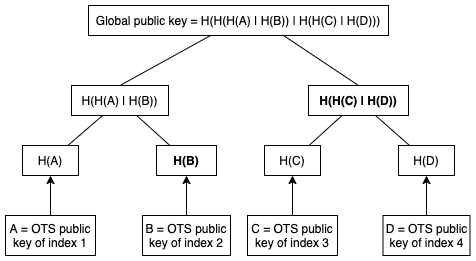
\includegraphics[scale=0.75]{img/merkle.png}}
% otherwise see the example in the following (commented out) line
% to scale it 50% (e.g. 20pt font get scaled to 10pt font)
%   \centerline{\includegraphics[scale=0.5]
% if you have a picture (i.e. no text hence no font size problem)
% you can fit it relatively to the page width
%   \centerline{\includegraphics[width=0.9\textwidth]
\caption{An example of a plain Merkle Tree with four leaves.}
\label{fig:merkle}
\end{figure}

An example of a plain Merkle tree is presented in \myfig{\ref{fig:merkle}}.
After signing a message with the first OTS (A), the authentication path would be the one highlighted in bold in the figure.
We can see that we can compute the global public key with the OTS public key A and the two hashes $H(B)$ and $H(H(C)|H(D))$, that are the neighbour nodes of all the nodes in the path from the signing leaf to the root of the Merkle tree. Thus we can verify that the obtained signature was originated from a Merkle tree with that specific global public key \cite{5_postquantum_signature_usecase}:
the root can be recomputed from the OTS public key of index i\footnote{Remember that to ensure that each OTS key pair is used only once, the OTS key pairs are used in a predefined order, for example using the leaves of the tree from left to right \cite{1_sphincspaper}.}
and the corresponding authentication path for the i-th OTS public key \cite{13_faultattacks}.
Exploiting the usage of the authentication path, it is not necessary to know all the OTS public keys to verify the global public key. This technique saves space and computation.

Also, the global public key value is the output of a selected hash function, thus typically it has a size of 32 bytes - common hash functions such as SHA-256 produce outputs of 32 bytes \cite{53_hbs}.
Moreover, the global private key instead is generally handled using a pseudo-random number generator, applied to a seed. In this way it is sufficient to store the seed value. OTS private keys can be directly derived afterwards from the seed value using that generator. In this way, the global private key can be small, typically 32 bytes.

Hence, this approach generates small signatures, small secret keys, exploiting pseudo-random generators, and small public keys \cite{1_sphincspaper}.
Unfortunately, as exposed in \cite{13_faultattacks}, this Merkle Signature Scheme has two main disadvantages \cite{53_hbs}:
\begin{itemize}
	\item First, key generation and signature time are exponential in the tree height h as the whole tree must either be stored or recomputed each time a signature is performed, to generate the structure from the seed \cite{1_sphincspaper}. The problem of tree traversal is critical to the signing performance;
	\item Second, the signer must keep track of the used OTS key pairs and this need makes the scheme stateful.
\end{itemize}

For the first point, some improvements have been designed so far \cite{1_sphincspaper}\cite{32_XMSS}. For what concerns the last point instead, it will be further analysed in the following section.

\subsection{Statefulness}
\label{sub:statefulness}

Most of hash-based algorithms are stateful. This means that the overall system requires users to remember a state. This is the case of a traditional Merkle's tree-based signature scheme \cite{2_SPHINCS+_round2}, such as the eXtended Merkle Signature Scheme (XMSS) \cite{33_RFC_XMSS} or the Leighton-Micali Signature (LMS) \cite{37_RFC_LMS}, another common HBS scheme.
Those are the most mature HBS schemes \cite{5_postquantum_signature_usecase}, but they do not fit standard APIs neither the standard definition of signatures in cryptography \cite{1_sphincspaper}: due to their stateful property the sign operation reads a secret key and a message and generates a signature, but it also generates an updated secret key (the secret key is updated at every signature). This means that if the update fails then security disintegrates \cite{1_sphincspaper} - \eg the update could fail if a key is copied from one device to another, or if it is backed up and later restored. 

The state could be represented by some information on how many signatures were already made with the key, in order to keep track of all produced signatures. Merkle's design of HBS strongly relies on iterating over signing keys in order \cite{3_SPHINCS_secondpaper}: since a stateful HBS is based on a one-time signature, the signer needs to ensure that the OTS private key is never reused.

Practically, it can be difficult to deal with a state. For instance when sharing a private key on different servers that wish to sign messages concurrently, one has to synchronise all of them or security is broken \cite{4_wings}.
The state management requirement is an important disadvantage, as stated by IETF and NIST \cite{5_postquantum_signature_usecase}, since it is not acceptable for many applications.
Moreover, if an adversary is able to manipulate the state, the security of the scheme degrades significantly \cite{12_faultinjection}.

To overcome these limitations, stateless signature schemes have been proposed, such as SPHINCS \cite{7_hashbased}. However, due to its stateless property, it produces larger signatures and is much less efficient than stateful signature schemes, like XMSS \cite{5_postquantum_signature_usecase}.
SPHINCS is built upon the theoretical work of Goldreich \cite{3_SPHINCS_secondpaper}, who proposed the first stateless HBS scheme.

The structure proposed by Goldreich is so large that, approximately, one can pick a signing key at random each time and can reasonably assume that the key has not been used before \cite{3_SPHINCS_secondpaper}. This is essential for many real-world scenarios, as the one previously mentioned of distributed servers, where continuously updating a stateful key pair is often impossible. 

SPHINCS improves this construction in several aspects. According to \cite{4_wings}, SPHINCS demonstrates that stateless schemes can be practical, even with a reduced overall performance, since it provides a reasonable signature size, of 41 KB, and is able to compute hundreds of signatures per second on a modern CPU.

We will focus on the stateless property of SPHINCS algorithm in Section \ref{subsub:stateless}.

\subsection{Advantages of hash-based}
\label{sub:advantages}

Summing up, the main advantage of hash-based signatures is that their security relies only on specific cryptographic properties of the underlying hash function. It follows that if the chosen hash function is broken one day, it can be easily replaced with a new one.

Besides, as explained in \cite{12_faultinjection}, from a quantum point of view, the effectiveness of generic attacks against hash functions can not exceed Grover's algorithm \cite{36_Grover}.
This is a quantum algorithm, invented in 1996, which finds with high probability the unique input to a black box function, given a particular output value, using at most $\sqrt{N}$ evaluations of the function, where N is the size of the domain of the function. 
In our case, the black box function is the hash function: Grover's algorithm is able to find a preimage x, given the hash function H and the hash value h, such that H(x) = h.
This means that a quantum adversary can not obtain more than a square-root speed-up compared to classic preimage search, in which the preimage is found at most with N evaluations, where N is the cardinality of the set of possible inputs \cite{12_faultinjection}. Since HBS schemes are based on hash functions, this result holds also for these schemes. 

Moreover, as described in \cite{1_sphincspaper}, hash-based signing is reasonably fast for stateful schemes, even without hardware acceleration. Verification is faster, since it directly exploits hash functions. For some hash-based signatures, like XMSS, signatures and keys are reasonably small.
This is not the case for the stateless schemes, like SPHINCS, since the stateless propriety does not come for free: it requires bigger keys, with an increase of both the signing time and the signature size \cite{8_ARM}. 

In addition, some hash-based signature schemes, like XMSS, are considered forward secure \cite{32_XMSS}, meaning that previous signatures remain valid if a secret key is compromised.

Until now, while the security of hash-based signatures has been fully analysed, their concrete integration in popular security protocols has not been addressed so far \cite{9_postquantum_auth_openssl}, mainly because most HBS schemes are stateful: requiring a state that must be constantly kept up to date is totally different from the signature schemes that are currently in use in many real-world scenarios \cite{8_ARM}. Indeed, the stateful property makes these algorithms, such as XMSS, not to fit the standard definition of signature schemes, as the definition stated in the NIST project \cite{2_SPHINCS+_round2}.
For this reason, we are going to focus on a new stateless HBS scheme, SPHINCS, in Section \ref{sec:sphincs}.

\section{SPHINCS}
\label{sec:sphincs}
%introduction and a bit of history

SPHINCS is a recently proposed stateless hash-based signature framework \cite{1_sphincspaper}.
Before it, all practical hash-based schemes required to keep track of a state. In many real-world use cases, a stateful signature scheme is problematic \cite{8_ARM}.
For this reason, in 2015, SPHINCS has been proposed, demonstrating that it is not strictly necessary to deal with a state for a hash-based scheme \cite{8_ARM}. Being stateless allows this scheme to be a suitable replacement for current signature schemes \cite{1_sphincspaper}.

It has been known for many years that one can theoretically build hash-based signature schemes without a state: this concept was first introduced by Goldreich in 2004 \cite{50_Goldreich}. 
However, SPHINCS is the first practical stateless hash-based signature scheme, which provides security against quantum attacks \cite{1_sphincspaper}.

SPHINCS is carefully designed so that its security can be based on weak standard-model assumptions of the underlying cryptographic hash function \cite{1_sphincspaper} and it exploits a randomised tree-based structure. With ``randomised" we mean that indexes are selected randomly rather than sequentially \cite{9_postquantum_auth_openssl}, as it happens for example with the traditional Merkle Signature Scheme.
However, the stateless property has some downsides: there is an increase in signing time and in signature size with respect to stateful schemes \cite{8_ARM}. 

More in details, the tree-based SPHINCS structure relies on HORS with trees (HORST), an improvement of the HORS few-time signature scheme that we analysed previously in section \ref{subsub:fts}. The usage of a few-time signature scheme instead of a one-time signature scheme is preferred since multiple signing with a given key pair does not cause a complete break in security as in one-time signature schemes, but results in a progressive shrinking of security \cite{9_postquantum_auth_openssl}.

In 2015 with the original submission of the algorithm \cite{1_sphincspaper}, an efficient high-security instantiation of SPHINCS has been proposed, SPHINCS-256. 
This was the first instantiation proposed and, according to \cite{1_sphincspaper}, it signs hundreds of messages per second on a modern 4-core 3.5GHz Intel CPU. Its signatures are 41 KB long, public keys and private keys are 1 KB long. The signature scheme, and in particular the SPHINCS-256 instantiation, is designed to provide long-term $2^{128}$ security even against quantum attackers \cite{1_sphincspaper}.
However, until now SPHINCS has not yet benefited from the extensive scrutiny that other HBS schemes did already undergo, such as the XMSS scheme \cite{9_postquantum_auth_openssl}.

In the following sections, we will describe the structure of the SPHINCS algorithm and analyse its main components.
In 2017, a new version of the SPHINCS scheme has been proposed. This enhanced version is called SPHINCS+, which, according to \cite{3_SPHINCS_secondpaper}, it has significant advantages over the state of the art in terms of speed, signature size, and security, and is among the nine remaining signature schemes in the second round of the NIST PQC standardisation project. For this reason, in section \ref{sub:sphincsplus}, we will introduce the main improvements introduced by this enhanced version and for the subsequent sections we will mainly focus on SPHINCS+.


\subsection{Definition of the algorithm: SPHINCS}
\label{sub:def}
% parte "introduttiva" dell'algoritmo

Before focusing on SPHINCS we want to give a general overview of XMSS, a stateful scheme relying on the MSS scheme. That is because we want to show what are the main differences and innovations introduced by SPHINCS in respect to most recent hash-based signature schemes, among which XMSS is the most common one.

Generally speaking, XMSS main construction looks like a Merkle tree with some differences.
The main problem of the Merkle tree signature scheme, described in section \ref{subsub:merkle}, is that key generation and signature time are exponential in the height h of the tree. As explained in \cite{1_sphincspaper}, XMSS solves these performance problems. Key generation time is significantly reduced using a hypertree of several layers of trees. In this way, during key generation only one tree on each layer has to be generated. The signature time instead is reduced with respect to MSS using stateful algorithms, that exploit the ordered use of the OTS key pairs. Combining hypertrees with the ordered use of trees the signing time is significantly reduced.


\begin{figure}
% If the picture uses fonts of the correct size (10 ... 12 pt)
% then it can be included without scaling
\centerline{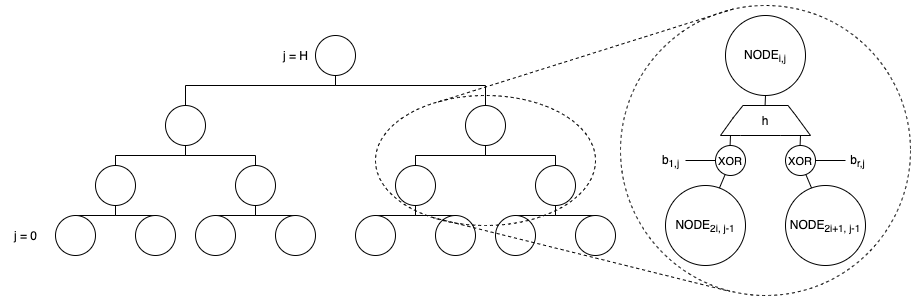
\includegraphics[scale=0.5]{img/xmss.png}}
% otherwise see the example in the following (commented out) line
% to scale it 50% (e.g. 20pt font get scaled to 10pt font)
%   \centerline{\includegraphics[scale=0.5]
% if you have a picture (i.e. no text hence no font size problem)
% you can fit it relatively to the page width
%   \centerline{\includegraphics[width=0.9\textwidth]
\caption{The XMSS hypertree structure.}
\label{fig:xmss}
\end{figure}

In order to look closer to the XMSS hypertree structure, \myfig{\ref{fig:xmss}} is presented \cite{53_hbs}. As illustrated in the figure, a XMSS tree has a mask - identified by the b letter in the figure, and that has a different value for every node - which is first XORed to the corresponding child node and then those results are hashed together in their parents node.
Another difference with Merkle trees is that a leaf of the XMSS is not a hash of a OTS public key, as it happened for the Merkle Signature Scheme, but it is the root of another tree called L-tree \cite{32_XMSS}.

A L-tree is not a full binary tree, but it is an unbalanced binary tree \cite{1_sphincspaper}.
This means that a node that has no right sibling is lifted to a higher level of the L-tree until it becomes the right sibling of another node \cite{32_XMSS}.

With this construction, it follows the same idea explained before: masks are applied to hash its nodes. This mask is different from the one of the main XMSS tree, but it is common to all the L-trees. Inside the leaves of each L-tree the elements of a WOTS+ public key are stored: therefore a L-tree is used to hash WOTS+ public keys \cite{1_sphincspaper}.
According to Huelsing, storing the WOTS+ public key makes possible to use a second-preimage resistant hash function, instead of a collision resistant one \cite{53_hbs}.
Finally, the global public key is composed of the root node of the XMSS tree, the bitmasks used in the XMSS tree and a L-tree.

\begin{figure}
% If the picture uses fonts of the correct size (10 ... 12 pt)
% then it can be included without scaling
\centerline{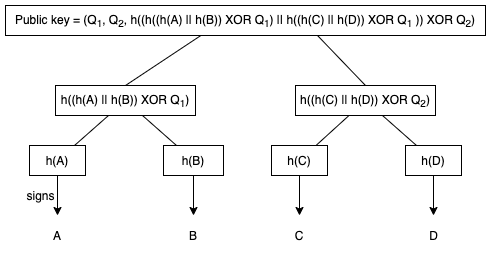
\includegraphics[scale=0.75]{img/firsttree.png}}
% otherwise see the example in the following (commented out) line
% to scale it 50% (e.g. 20pt font get scaled to 10pt font)
%   \centerline{\includegraphics[scale=0.5]
% if you have a picture (i.e. no text hence no font size problem)
% you can fit it relatively to the page width
%   \centerline{\includegraphics[width=0.9\textwidth]
\caption{The first tree of the SPHINCS hypertree structure.}
\label{fig:firsttree}
\end{figure}

Given this, we want to introduce SPHINCS. It is the most recent hash-based signature scheme and it is stateless \cite{53_hbs}. SPHINCS is based on many trees. The first tree is showed in \myfig{\ref{fig:firsttree}} . This structure is very similar to the Merkle tree one described in Section \ref{subsub:merkle}, with additional bitmasks. Because of this addition, we will always refer to these SPHINCS trees as binary hash trees, to differentiate them from the plain Merkle tree structure.
As it happens in the XMSS scheme, each node is computed hashing the concatenation of the previous nodes - the child nodes - XORed with a level bitmask. The level bitmask is different for each level, but it is the same for each node of a fixed level.
The public key of the first tree is the root, computed as before hashing the result of the XOR operation between the level bitmask and the concatenation of the child nodes, along with the bitmasks for all the levels of this tree ($Q_{1}$ and $Q_{2}$ in the figure).
The leaves of the tree are the hashed public keys of WOTS+ L-trees.
The WOTS+ L-trees are similar to the XMSS L-trees of before, except that their bitmask is unique per level.
Each leaf, containing one WOTS+ signature, allows to sign another tree. Hence now there is a second layer of four SPHINCS trees, containing themselves WOTS+ public keys at their leaves. This procedure is iterated according to some initial parameters, that we will present later. Finally, at layer 0, the WOTS+ signatures will not sign other SPHINCS trees but HORST structures.
A HORST or HORS Tree is like a L-tree but containing a HORS few-time signatures instead of a Winternitz one-time signature. Those HORST structures will be used to sign messages. Exploiting FTS instead of OTS schemes increases the security of the scheme since signing a message with the same HORS key does not break the scheme itself.

To sign a message m, the signer first creates a ``randomised" hash of m and a ``random" index. Since in SPHINCS everything is deterministic, those ``randomised" values are actually computed with a Pseudo Random Function (PRF). The index indicates which HORST must be picked to sign the randomised hash of m. Picking the index deterministically according to a message makes the scheme stateless: signing the same message again should use the same HORST, while signing two different messages should make use of two different HORSTs. 

Before going into the details of the SPHINCS scheme that we explained so far, we will describe its components in order to have a clearer understanding of the building blocks of this scheme. Those components will be described in the next sections following the presented order:
\begin{enumerate}
	\item First we will focus on the stateless construction, which was invented by Goldreich, who proposed the first HBS scheme: the stateless SPHINCS construction evolves directly from this scheme;
	\item Then, we will have a brief recap on the one-time signature scheme exploited in SPHINCS, the WOTS+ scheme, that we presented in section \ref{subsub:ots};
	\item We will provide an overview on binary hash trees used by SPHINCS. These trees are similar to the classical binary Merkle trees, exposed in section \ref{subsub:merkle}, but their construction has been slightly modified, with respect to traditional Merkle trees, in the SPHINCS context;
	\item Later, we will present the few-time signature scheme HORST, the principal component of the SPHINCS scheme. Note that HORST is the evolution of the HORS scheme described in section \ref{subsub:fts};
	\item Finally we will present the SPHINCS many-time signature scheme, describing its key generation procedure, its signature and verification algorithms, and summarising its main parameters.
\end{enumerate}


\subsubsection{Goldreich's construction}
\label{subsub:stateless}

As explained in Section \ref{sub:statefulness}, most of the practical HBS schemes are stateful, meaning that a state needs to be maintained as a part of the secret key \cite{12_faultinjection}.
While this is not a problem in some applications, having to maintain a state for digital signature schemes can have several negative consequences. In scenarios where there are multiple instances of the key stored in different places - as what happens for backups, management of distributed servers or management of different devices owned by the same user -, the state needs to be constantly synchronised among those copies \cite{8_ARM}. This makes stateful schemes highly impractical and not suitable for many real-world scenarios.

All of those stateful schemes are improvements of the Merkle Signature Scheme introduced in section \ref{subsub:merkle}, like the XMSS scheme explained in the previous section.
The design of the Merkle Signature Scheme heavily relies on iterating over signing keys in order, avoiding the reuse of the same signing key \cite{3_SPHINCS_secondpaper}.

Already in 1986, Goldreich recognised the problem of having a stateful scheme and proposed a solution. He proposed to create a tree of such depth that, roughly, one can pick a OTS key pair randomly for each signature and reasonably assume it has not been used before \cite{3_SPHINCS_secondpaper}: with a sufficient large structure, the probability of reusing a certain OTS key pair becomes insignificantly small \cite{8_ARM}.
In this way, there is no need to keep track of the OTS keys already used to sign messages.
The problem of this solution is how to create such a large tree.
He proposed to avoid computing the entire tree: instead of simply hashing nodes together, as for the typical Merkle tree construction, in Goldreich trees an OTS key pair is attached to each tree node and is used to sign the child nodes \cite{8_ARM}. This can be realised if and only if the OTS keys of the nodes along the path, starting from a random leaf and arriving to the root node, are deterministically generated: this can be done exploiting a pseudorandom function with a secret seed and the index of the node as inputs \cite{8_ARM}.

Upon this idea, later in 2004, Goldreich proposed a stateless hash-based signature scheme \cite{50_Goldreich}, based on a binary tree of one-time signatures.
As explained in \cite{7_hashbased}, each node of this tree corresponds to an OTS instance. Each internal node, which corresponds to each non-leaf node, authenticates the public keys of its two child nodes by means of the OTS. For example, the OTS of node i signs $(pk_{left(i)}, pk_{right(i)})$ with the secret key $sk_{i}$. The global public key is the OTS public key of the root node.
The leaf OTS key pairs are used to sign the messages.
The secret key is a seed value that is used to generate all the OTS key pairs of the tree pseudorandomly\footnote{Note that the pseudo random function should be deterministic for a given seed, thus the consistency of the scheme is guaranteed.}: each OTS instance is generated by a pseudo random generator taking as argument this seed and the index i of the node inside the tree \cite{7_hashbased}.
In this way, the tree is generated on demand, since the root node needs to be computed only at key generation time, and only the nodes on the path need to be computed for each signature. 

Since the scheme is constructed upon one-time signatures, it is important to ensure that a single key pair is never used to sign two different messages. This constraint is automatically verified for internal nodes, that only sign the public keys of their children, but it must be enforced for each OTS leaf. In other words, the path, identified by the symbol $\rho$, must be different for every message. Goldreich proposed to use a random path $\rho$ for every message \cite{7_hashbased}.
In this way, to sign a message a OTS leaf is selected randomly: instead of applying a public hash function to the message to determine the index of the OTS key pair, the index is selected randomly.
Following this construction, given a tree of height h, the full signature of the message m contains \cite{1_sphincspaper}:
\begin{enumerate}
	\item The path $\rho=(\rho_{1},...,\rho{h})$, where $\rho_{i}$ is a bit which indicates left or right node;
	\item The authentication path A, composed by the authentication $A_{i}$ for each h layer. Each $A_{i}$ is computed with all the OTS public keys in the path $\rho$, from leaf h to the root, and all the public keys of the sibling nodes on this path, signed with the secret key for the i layer. The formula is $A_{i}=sign(sk_{\rho_{i}}, (pk_{left(\rho_{i})},pk_{right(\rho_{i})}))$;
	\item The one-time signature $\sigma$ of the message computed with the leaf belonging to the path $\rho$, $\sigma=sign(sk_{\rho_{h}}, m)$.
\end{enumerate}

Basically, the Goldreich scheme replaces ``hashing" with ``signing" throughout the tree and replaces hash digests with OTS signatures for the nodes in the authentication path included in each signature \cite{8_ARM}. For this reason, the main drawback of this approach is the signature size: the parameters required for this construction, in order to provide a sufficient security level and a reasonable number of signatures per key pair, produce signatures of above 1 MB \cite{4_wings}.
According to \cite{1_sphincspaper}, a signature size like this would dominate the traffic in many applications, such as in operating system updates or in HTTPs connections to an average sized web page.
Since the Goldreich scheme is highly inefficient, due to its huge signature size, the SPHINCS approach has been introduced in order to drastically reduce signature size \cite{1_sphincspaper}. We will present it in section \ref{subsub:sphincs_construction}.

\subsubsection{WOTS+}

We will now recall the Winternitz one-time signature variant (WOTS+) scheme. It is a one-time signature scheme, hence the private key must be used to sign exactly one message. When it is reused, security degenerates \cite{3_SPHINCS_secondpaper}.

This variation of WOTS is designed to reduce the signature size.
As in WOTS the Winternitz parameter $w = 2^{W}$ is used to configure the trade-off between the signature size and the number of computations \cite{4_wings}.
A small value of w leads to a faster scheme, but results in larger keys and signatures. This happens because the scheme signs W bits at once by hashing at most $2^{W} - 1$ times a secret value \cite{12_faultinjection}.

We will describe the algorithms as they are used in SPHINCS. Specifically we include pseudorandom key generation and fix the message length to be n, meaning that a seed value takes the place of a secret key in our description. 
Given n and w, we define:

$$l_{1} = \lceil {\frac{n}{\log w}} \rceil $$

$$l_{2} = \lfloor \frac{\log (l_{1}(w-1))}{\log w} \rfloor + 1$$

$$l = l_{1} + l_{2}$$

Making an example, for obtaining $n=256$ bits of security $l$ is equal to 67.

In the standard WOTS scheme, a function F is applied to the secret key several times to produce a hash chain. In the WOTS+ scheme, also bitmasks are involved in this process \cite{8_ARM}.

Given that F is a second-preimage resistant hash function, at every iteration, before applying F, the input is XORed with a iteration-specific bitmask $r_{i}$. The chaining function then looks as follows, where the base case is $c^{0}(x,r) = x$  \cite{8_ARM}:
$$c^{i}(x,r) = F(c^{i-1}(x, r) \oplus r_{i})$$
given that i is the iteration counter.
Thus, in every iteration, the function first takes the bitwise XOR of the previous value $c^{i-1}(x, r)$ and bitmask $r_{i}$ and evaluates F on the result \cite{1_sphincspaper}.

For the sake of clarity, $r_{a,b}$ stands for the substring $(r_{a} , . . . , r_{b})$ of r. In case $b < a$, $r_{a,b}$ is the empty string \cite{1_sphincspaper}.

Now we describe WOTS+ key generation, signature and verification algorithms \cite{1_sphincspaper}:

\begin{enumerate}
	\item \textbf{Key Generation} ($sk, pk \gets WOTS.kg(S, \textbf{r})$):
	Given as input a seed $S \in \{0, 1\}^{n}$ to a pseudo random generator G, the key generation algorithm computes the internal secret key as $sk = (sk_{1} , . . . , sk_{l}) \gets G_{l}(S)$: the n bit seed is expanded to $l$ values of n bits.
	Giving also bitmasks $r \in \{0, 1\}^{n \times (w-1)}$, the public key is then computed by applying the chaining function on each part of the secret key \cite{4_wings}: 
	$pk = (pk_{1} , . . . , pk_{l} ) = (c^{w-1}(sk_{1},r), . . . , c^{w-1}(sk_{l},r))$.
	In this way, the generation of sk and pk can be done on the fly when necessary. Note that S requires less storage than sk.
	\item \textbf{Signature} ($\sigma \gets WOTS.sign(M, S, \textbf{r}$): Given a message M of length n, the seed S and the bitmasks r, the signature algorithm first computes a representation in base w of M: $M = (M_{1} . . . M_{l_{1}})$, $M_{i} \in \{0, . . . , w - 1\}$. Here M is treated as the binary representation of a natural number x and then the representation of x in base w is computed.
	Next it computes the checksum $C=\displaystyle\sum_{i=1}^{l_{1}} (w - 1 - M_{i})$ and its base w representation $C = (C1 , ..., C_{l_{2}})$. The length of this base w representation of C is at most $l_{2}$ since $C \leq l_{1}(w - 1)$.
	This checksum is necessary to prevent message forgery since an increase in at least one $M_{i}$ leads to a decrease in at least one $C_{i}$ and vice-versa \cite{3_SPHINCS_secondpaper}.
	Concatenating these values we obtain $B = (b_{1} , . . . , b_{l} ) = M \parallel C$. Then the internal secret key is generated using $G_{l}(S)$, in the same way as during the key generation phase.
	The signature is computed as $$\sigma = (\sigma_{1} , . . . , \sigma_{l}) = (c^{b _{1}}(sk1, \textbf{r}),..., c^{b_{l}}(sk_{l}, \textbf{r})).$$
	\item \textbf{Verification} ($pk' \gets WOTS.vf(M, \sigma, \textbf{r})$): Given an input message M of length n, a signature $\sigma$ and bitmasks \textbf{r}, the verification algorithm computes the $b_{i}$ , $1 \leq i \leq l$ as described above. Then it computes the public key as follows:
	$$pk' = (pk'1, ..., pk'l ) = (c^{w-1-b_{1}}(\sigma_{1}, \textbf{r}_{b_{1}+1,w-1}), . . . , c^{w-1-b_{l}}(\sigma_{l},\textbf{r}_{b_{l}+1,w-1})).$$
	The correct bitmasks have to be used in each step of the chaining function to get the correct results. The final step is to check whether pk' = pk \cite{4_wings}.
\end{enumerate}


\subsubsection{Binary hash trees and L-trees}

For this section, we start from the construction proposed for the XMSS already mentioned in Section \ref{sub:def}.
The central elements of the SPHINCS construction are full binary hash trees \cite{1_sphincspaper}, with a similar structure with respect to the XMSS one, showed in \myfig{\ref{fig:xmss}}. The main difference is that, in SPHINCS, nodes $NODE_{2i, j-1}$ and $NODE_{2i+1, j-1}$ are first concatenated and then their concatenation is XORed with a bitmask $Q_{j}$, unique for each level j.

Given that, we can go more in details.
In SPHINCS a binary hash tree of height h always has $2^{h}$ leaves. Each leaf is a n bit string $L_{i}$, where $i \in [2^{h} - 1]$.
Each node $N_{i,j}$ of the tree, for $0 < j \leq h, 0 \leq i < 2^{h-j}$, stores an n-bit string \cite{1_sphincspaper}.
To construct the tree, h bitmasks $Q_{j} \in \{0, 1\}^{2n}$, where $0 < j \leq h$, are used. For the leaf nodes we define $N_{i,0} = L_{i}$.
The values of the internal nodes $N_{i,j}$ are computed as follows \cite{1_sphincspaper}:

$$N_{i,j} = H((N_{2i,j-1} \parallel N_{2i+1,j-1}) \oplus Q_{j})$$

The root is denoted as $ROOT = N_{0,h}$.

Moreover, also the authentication path $Auth_{i} = (A_{0} , . . . , A_{h-1})$ of a leaf $L_{i}$ is needed. $Auth_{i}$ consists of all the sibling nodes of the nodes contained in the path from $L_{i}$ to the root. 
Given a leaf $L_{i}$ together with its authentication path $Auth_{i}$, the root of the tree can be easily computed \cite{1_sphincspaper}.

In addition to the full binary trees described above, SPHINCS uses also unbalanced binary trees called L-Trees \cite{1_sphincspaper}. They are used exclusively to hash WOTS+ public keys. The $l$ leaves of an L-Tree are the elements of a WOTS+ public key and the tree is constructed as described above but with one difference, which makes the tree unbalanced: a left node that has no right sibling is lifted to a higher level of the L-Tree until it becomes the right sibling of another node. Then all the computations work the same as for binary trees \cite{1_sphincspaper}. In the end, since L-Trees have height $\lceil \log l \rceil$, they need $\lceil \log l \rceil$ bitmasks.

\subsubsection{HORST}

The other important component of SPHINCS is the few-time signature scheme. SPHINCS uses HORST, which is a variant of HORS with an additional tree structure.
In respect to HORS, HORST sacrifices runtime to reduce the public key size and the total size of a signature and a public key \cite{1_sphincspaper}.

As HORS, HORST has two parameters $t = 2^{\tau}$ and $k$ \cite{4_wings}.
Formally, a HORST public key is the root node of a binary hash tree of height $\log t$, where the leaves are the public key elements of a HORS key. Thus, the public key size consists of a single hash value. In order to have this reduced key size, a HORST signature contains both the k secret key elements and one authentication path per secret key element. In this way the public key can be computed given a signature. Finally, a full hash-based signature includes just $k\log t$ hash values, while a HORS signature contains t hash values \cite{1_sphincspaper}.

The algorithms for HORST are the following \cite{1_sphincspaper}:

\begin{enumerate}
	\item \textbf{Key generation} ($pk \gets HORST.kg(S, Q)$): Given as input a seed $S \in \{0, 1\}^{n}$ and bitmasks $ Q \in \{0, 1\}^{2n \times \log t}$ the key generation algorithm first computes the internal secret key using a pseudo random function G: $sk = (sk_{1} , . . . , sk_{t} ) \gets G_{t}(S)$. The elements of this list are used to generate the leaves of a binary tree $L_{i} = F(sk_{i})$ for $i \in [t - 1]$.
	On top of these leaves a hash tree is computed using bitmasks Q. The public key pk is then computed as the root node of this binary tree of height $\log t$.
	\item \textbf{Signature} ($(\sigma, pk) \gets HORST.sign(M, S, Q)$). Given a message $M \in \{0, 1\}^{m}$, a seed $S \in \{0, 1\}^{n}$, bitmasks $Q \in \{0, 1\}^{2n \times log t}$ and the internal secret key sk computed as above, first the message is split into k pieces of length $\log t$, obtaining $M = (M_{1} , . . . , M_{k} )$, in which each $M_{i}$ is seen as an unsigned integer.
	Next, we compute the signature $\sigma = (\sigma_{0} , . . . , \sigma_{k-1} ,\sigma_{k})$, which consists of k blocks $\sigma_{i} = (sk_{M_{i}}, Auth_{M_{i}})$ for $i \in [k -1]$: each block contains the $M_{i}$th secret key element and the lower $\tau - x$ elements of the authentication path of the corresponding leaf $(A_{0} , . . . , A_{\tau - 1 - x})$. Thus the block $\sigma_{k}$ contains all the $2^{x}$ nodes of the binary tree on level $\tau - x$. In addition to the signature, the signature algorithm also outputs the public key.
	\item \textbf{Verification} ($pk' \gets HORST.vf(M, \sigma, Q)$): Given the message M, the signature $\sigma$ and bitmasks Q, this algorithm computes the $M_{i}$, as described above. After that, it computes the $2^{x}$ nodes of the tree already computed during the signature phase, using as input the message M, the leaf nodes and the corresponding authentication path. Then the algorithm compares each computed node to the nodes in $\sigma$. If all comparisons are correct, the algorithm uses $\sigma_{k}$ to compute $ROOT_{0}$.
\end{enumerate}

\subsubsection{SPHINCS construction}
\label{subsub:sphincs_construction}
% recap

We can now build the entire SPHINCS structure starting from the components we explained so far.
As described in \cite{1_sphincspaper}, a SPHINCS key pair defines a ``virtual" structure. SPHINCS considers the Goldreich's construction as a hypertree with h layers, in which each layer is a tree of height 1. Starting from it, SPHINCS generalises this idea to a hypertree of height h, with d layers of binary hash trees of height h/d. Each of these trees has the following structure: the leaves of a tree are $2^{h/d}$ L-Tree root nodes, and each compress the public key of a WOTS+ key pair. 

Therefore, a tree can be viewed as a key pair that can be used to sign $2^{h/d}$ messages. The hypertree is structured into d layers. On the top layer $d-1$ there is one single tree. The second layer $d-2$ has $2^{h/d}$ trees.
The roots of these trees are signed using the WOTS+ key pairs of the tree on layer $d-1$. Iterating this procedure for all layers, we have that layer i has $2^{(d-1-i)(h/d)}$ trees and the roots of these trees are signed using the WOTS+ key pairs of the trees on layer i+1.
At the bottom of the tree, on layer 0, each WOTS+ key pair is used to sign a HORST public key.

\begin{figure}
% If the picture uses fonts of the correct size (10 ... 12 pt)
% then it can be included without scaling
\centerline{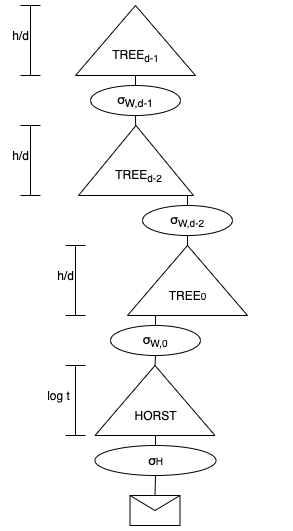
\includegraphics[scale=0.6]{img/sphincs.png}}
% otherwise see the example in the following (commented out) line
% to scale it 50% (e.g. 20pt font get scaled to 10pt font)
%   \centerline{\includegraphics[scale=0.5]
% if you have a picture (i.e. no text hence no font size problem)
% you can fit it relatively to the page width
%   \centerline{\includegraphics[width=0.9\textwidth]
\caption{The virtual structure of a SPHINCS signature \cite{1_sphincspaper}.}
\label{fig:sphincs}
\end{figure}

This structure is defined as ``virtual" because all values are determined choosing a seed and the bitmasks, while the complete structure is never computed.
The seed is part of the secret key and, as we will see in the key generation algorithm, it is used by the pseudorandom function.
An example of this virtual structure is shown in  \myfig{\ref{fig:sphincs}}, illustrating the path from the HORST chosen to sign a message to the root node.


Summing up, the WOTS+ signatures and authentication paths from a leaf at the bottom of the hypertree to the root of the top-most tree constitutes an authentication path \cite{3_SPHINCS_secondpaper}. Following this authentication path, each tree authenticates the tree below using a WOTS+ signature $\sigma_{W,i}$, in which W indicates that is a WOTS+ signature and i is the layer in the tree. In the last layer, the tree authenticates a HORST public key using a WOTS+ signature.
Finally, this last HORST key pair is used to sign the message.
The trees inside the hypertree used - that define the WOTS+ key pairs used for the signature - and the HORST key pair are determined by a pseudorandomly generated index \cite{1_sphincspaper}.
This index uniquely identifies an address for each leaf of the structure: the address contains the layer of the leaf in the SPHINCS hypertree, the number of the binary hash tree tree to which it belongs inside the hypertree layer and its position inside the binary hash tree \cite{13_faultattacks}.

By using a few-time signature scheme as HORST rather than a one-time signature scheme, SPHINCS does not require the same amount of leaf nodes to maintain the same security level: the probability of selecting the same node repeatedly can be much higher without breaking the system \cite{8_ARM}.

Now we can describe the key generation, signature and verification algorithms of the SPHINCS construction \cite{1_sphincspaper}:

\begin{enumerate}
    \item \textbf{Key generation} ($(SK, PK) \gets kg(1^{n})$). The key generation algorithm first generates two secret key values $(SK_{1} , SK_{2}) \in \{0, 1\}^{n} \times \{0, 1\}^{n}$.
    The value $SK_{1}$ is used for pseudorandom key generation. The value $SK_{2}$ is used in the signature algorithm to generate an index and pseudorandom values in order to randomise the message hash.
    Furthermore, we need to generate all the bitmasks Q for WOTS+ and HORST instances and for binary hash trees\footnote{Notation: following the original paper \cite{1_sphincspaper}, we use $Q_{WOTS+}$ for the first w - 1 bitmasks of length n inside Q related to the WOTS+ structures, $Q_{HORST}$ for the first $2\log t$ bitmasks related to the HORST structures, $Q_{L-Tree}$ for the first $2\lceil \log l\rceil$ bitmasks, and $Q_{Tree}$ for the $2h$ strings of length n in Q that follow $Q_{L-Tree}$ respectively for binary hash trees and L-trees in the SPHINCS virtual structure.}.
    Then the key generation algorithm has to generate the root node of the tree on the first layer d - 1.
    For this reason the WOTS+ key pairs for the single tree on layer d - 1 are generated. The seed $S_{A}$ for a WOTS+ key pair with address A is computed giving to the pseudo random function the address A and the $SK_{1}$ as inputs. This happens also for the single tree on layer d - 1.
    The WOTS+ public key is computed as follows:
    $pk_{A} \gets WOTS.kg(S_{A} , Q_{WOTS+})$.
    The \textit{i}th leaf $L_{i}$ of the tree is the root of an L-Tree which compresses $pk_{A}$ using the bitmasks $Q_{L-Tree}$ . In the end, a binary hash tree is built using the constructed leaves and the root node becomes $PK_{1}$.
    Finally, the key generation algorithms returns the key pair (SK, PK), where the secret key is $SK = (SK_{1}, SK_{2}, Q)$ and the public key is $PK = (PK_{1}, Q)$.
    \item \textbf{Signature} ($ \Sigma \gets sign(M, SK)$). The first step is to select a HORST key to sign the message.
    Given as input a message $M \in \{0, 1\}^{*}$ and the secret key $SK=(SK_{1}, SK_{2}, Q)$, a pseudorandom $R=(R_{1}, R_{2}) \in \{0,1\}^{n} \times \{0,1\}^{n}$ is computed as $R \gets F(M, SK_{2})$, where F is a pseudo random function. Using the first n bits of R, a digest D of length m is generated as a randomised hash as follows: $D \gets H(R_{1}, M)$. The latter n bits of R are used to select the HORST key pair, exploiting an index i, computed from $R_{2}$ and h, which is the height of the hypertree. Note that since we use a pseudo random function, signing is deterministic. The HORST signature and public key are computed like this: $(\sigma_{H}, pk_{H}) \gets (D, S_{A_{HORST}}, Q_{HORST})$, with the HORST related bitmasks and the seed computed with the address $A_{HORST}$ and the first part of the secret key $SK_{1}$.
    The full SPHINCS signature contains, besides index i, the first random value $R_{1}$ and HORST signature $\sigma_{H}$, also one WOTS+ signature $\sigma_{W,i}$ and one authentication path $Auth_{A_{i}}$ per layer, for $0 \leq i \leq d-1$. In order to generate those signature, all necessary WOTS+ pubic keys need to be generated at runtime.
    The first step is to generate the WOTS+ key pair which signs the HORST public key used when computing $\sigma_{H}$. Hence the WOTS+ key pair with address $A_{0}$ is used to sign $pk_{H}$, using the relative bitmasks, obtaining $\sigma_{W,1} \gets (pk_{H} , S_{A_{0}} , Q_{WOTS+})$.
    The public key for this WOTS+ signature is part of another tree and therefore needs to be authenticated again \cite{4_wings}: for this reason the authentication path of the used WOTS+ key pair is computed.
    This procedure of signing the root with a WOTS+ key pair and computing the authentication path is repeated until the top layer is reached \cite{4_wings}.
    Finally, the full signature is $$\Sigma = (i, R_{1}, \sigma_{H} , \sigma_{W,0} , Auth_{A_{0}} , . . . , \sigma_{W,d-1} , Auth_{A_{d-1}}).$$
    \item \textbf{Verification} ($b \gets vf(M, \Sigma, PK)$). Given as input the message M, the signature $\Sigma$ and the public key PK, first the verification process recomputes the randomised digest for the message, using the randomness $R_1$ contained in the signature. Then the digest D and the HORST bitmasks $Q_{HORST}$ are used to compute the HORST public key, which can be used to verify $\sigma_{HORST}$.
    Then the HORST public key is used together with the WOTS+ bitmask and with the WOTS+ signature to compute the corresponding WOTS+ public key $pk_{W,0}$. Going on with each WOTS+ public key computed, the successive one is computed combining it with the next WOTS+ signature and the WOTS+ bitmask. In this way, the algorithm verifies $\sigma_{W,1}$ and all further signatures $\sigma_{W,i}$ until the root of the tree is reached. If all verifications succeed and the root of the top tree equals $PK_{1}$ the signature is accepted and the algorithm returns the boolean value true, otherwise it returns false \cite{4_wings}.
\end{enumerate}

We now summarise SPHINCS main parameters, following the notation in \cite{1_sphincspaper}: SPHINCS uses a hypertree of total height h, where h is a multiple of d and the hypertree consists of d layers of trees, each having height h/d. Additional parameters, that influence performance and size of the signature and keys, are the Winternitz parameter w for the WOTS+ components and the parameters k and $t=2^{\tau}$, where $k\tau = m$.

In order to provide practical values for these parameters, we present SPHINCS-256. 
SPHINCS-256 is the main implementation of SPHINCS, which provides 128 bits of security against quantum attackers, according to \cite{1_sphincspaper}.
For SPHINCS-256, the values are: $n = 256$, $m = 512$, $h = 60$, $d = 12$, $w = 16$, $t = 2^{16}$ , $k = 32$.
With these values, SPHINCS demonstrates that stateless schemes can be practical, providing a reasonable signature size of 41 KB and computing hundreds of signatures per second on a modern CPU \cite{7_hashbased}\cite{4_wings}.

\subsection{Updated algorithm: SPHINCS+}
\label{sub:sphincsplus}
% General enhancements

The SPHINCS scheme previously described has been enhanced in 2019, with a new submission to the NIST post-quantum crypto project \cite{2_SPHINCS+_round2}. 
This new submission proposed SPHINCS+. SPHINCS+ works as SPHINCS in its high level design but some of the internal components have been slightly modified.

The goal of SPHINCS+ is to improve the original scheme in terms of speed and signature size. This goal is achieved by introducing several improvements that strengthen the security of the scheme. 
The main modifications made to SPHINCS are the usage of a new few-time signature scheme called FORS and the way in which leaf nodes are chosen. These two changes together make the whole schema harder to attack via the few-time signature scheme, strengthening its security level, and hence allow to choose smaller parameters for the algorithm. These modifications were feasible thanks to the large flexibility offered by the many options of parameters.
Another important improvement is the introduction of tweakable hash functions. The properties of tweakable hash functions allow for a security analysis of the SPHINCS+ schema \cite{3_SPHINCS_secondpaper}.

In the next section we will present the main enhancements introduced by SPHINCS+.

\subsubsection{Enhancements}
% Detailed enhancements

SPHINCS+ introduces several improvements upon SPHINCS. In the following, the main ones will be presented \cite{2_SPHINCS+_round2}\cite{3_SPHINCS_secondpaper}:
\begin{itemize}
	\item \textbf{Multi-target attack protection and tweakable hash functions}. A multi-target attack is an attack on many users of a cryptosystem at once. Specifically to hash function, if an adversary obtains the keyed hash for the same input hashed with different keys, he could recover one or more keys. To protect from this attack, a mitigation technique has been proposed in \cite{51_MultiTarget} in 2016, which has been later implemented in SPHINCS+.
	The basic idea is to use a different hash function for each call. Moreover, each hash function call is keyed with a different key and applies different bitmasks. Keys and bitmasks are generated by a pseudo random function from an address specifying the context of the call and a public seed.
	Since this procedure is complex, the goal is to abstract away the details of how exactly nodes are computed, through hash function calls, from the high-level construction of the SPHINCS+ scheme.
	To get this abstraction they introduced the notion of tweakable hash functions, that in addition to the input value take as inputs a public seed and an address.
	Therefore, to mitigate the multi-target attack, SPHINCS uses two pseudo random functions, a keyed hash function and several tweakable hash functions. One pseudorandom function is for pseudorandom key generation, and the other one is used to generate randomness for the message compression.
	The keyed hash function instead is used to compress the message, since it can process arbitrary length messages.
	Formally, a tweakable hash function is defined as an efficient function mapping an $\alpha$-bit message M to an n-bit digest using a function key called public parameter P and a tweak T. In SPHINCS+ the public parameter P is a public seed which is part of the SPHINCS+ public key, while tweaks T are used to define the context. A hash function address is used as a tweak T, which identifies the position of the hash function call within the virtual structure defined by a SPHINCS+ key pair. In this way the hash function calls for each SPHINCS+ key pair and for each position in the virtual tree structure are independent from each other.
	\item \textbf{Tree-less WOTS+ public key compression}. The last nodes of the WOTS+ chains are not compressed using an L-tree but using a single tweakable hash function call. As previously explained, the hash function call receives an address and a public seed as a key for this call. With these two values the call also generates a bitmask of the same length of the input.
	Now bitmasks are generated pseudorandomly, therefore they have no influence on the public key size, while bitmasks in the original SPHINCS scheme accounted for a big part of the public key size.
	\item \textbf{Forest Of Random Subsets (FORS)}. The few-time signature scheme HORST has been replaced and improved by FORS. FORS uses as parameters k and $t=2^{a}$.
	While a HORST structure consists of a single tree, a FORS key pair consists of k trees of height $a = \log t$.
	The leaves of these trees are the hashes of t secret key elements: the total private key has $kt$ elements, grouped together into k sets of t values each. In the context of SPHINCS+, these values are deterministically derived from the main private seed in the SPHINCS+ private key, using a pseudo random function and the address of the key in the hypertree.
	Moreover, the public key of the entire FORS structure is the tweakable hash of the concatenation of all the root nodes: with the same construction of the WOTS+ public key, the root nodes are compressed into a n-bit value FORS public key.
	Differently than with HORST, FORS offers a dedicated set of secret key values per index derived from the message. Using the same parameters as for HORST, this leads to an increase of the key size and a decrease of the speed. But the advantage of FORS is that it is possible to use much smaller parameters to provide the same security level. Hence, in the end, we obtain an improvement in terms of signature size and speed, with respect to HORST.
	In order to have a FORS signature, given a message of $ka$ bits, $k$ strings of $a$ bits are extracted from the message. Each of these bit strings is interpreted as the index of a single leaf node in each one of the k FORS trees. The signature is constructed by these nodes and their respective authentication paths.
	The verification process then reconstructs each of the root nodes using the authentication paths and uses the tweakable hash to reconstruct the public key.
	In the SPHINCS+ context, a FORS signature is never verified explicitly, because the computed public key is used as a message which is implicitly checked together with a WOTS+ signature.
	\item \textbf{Verifiable index selection}. In the original SPHINCS algorithm the HORST key pair used to sign the message was selected generating an index in a pseudorandom manner. Since a secret seed value was involved, a verifier was unable to check if that index was actually generated in this way. For this reason, an adversary targeting the HORST scheme could mount a multi-target attack, using a single hash computation to target all HORST instances at the same time.
	This is not possible with SPHINCS+, since the computation of the index i is done together with the computation of the message digest d: $( m \parallel i ) = H (R, PK, m)$. In this formula, PK is the SPHINCS+ public key, which contains the top root node and the public seed, and R is the pseudo randomly generated value which becomes part of the signature. Hence, every message that an adversary tries becomes now directly linked to a single FORS instance and is not usable for any other instances.
	This new method of selecting the index is publicly verifiable, avoiding multi-target attacks on the FTS scheme: it prevents an attacker from selecting an index not pseudo randomly generated and from combining it with a chosen message.
	In addition, as the index can now be computed by the verifier, it allows to omit the index i in the SPHINCS+ signature.
\end{itemize}

Considering all these enhancements, we summarise how the SPHINCS+ scheme looks like in a more general way \cite{3_SPHINCS_secondpaper}.
First, the public key consists of two n-bit values: the root node of the top tree in the hypertree and a random public seed. In addition, the private key consists of two more n-bit random seeds: one seed used to generate the WOTS+ and FORS secret keys, and another one used for the randomised message digest.
Then, the SPHINCS+ signature consists of a FORS signature on the digest of the message, a WOTS+ signature on the corresponding FORS public key, and all authentication paths and WOTS+ signatures needed to authenticate the WOTS+ public key used for authenticating FORS.
To verify the chain of authentication paths and signatures, the verification algorithm iteratively reconstructs the public keys and root nodes until it reaches the root node at the top of the SPHINCS+ hypertree.

Recalling all parameters introduced so far, a summary of them is presented in \mytab{\ref{tab:parameters}}. This table will be useful for understanding the meaning of each SPHINCS+ variant identifier which will be used in the testbed results in Section \ref{sec:test}.

\begin{table}[]
\centering
\begin{tabular}{@{}lcccccccccc@{}}
\toprule
\textbf{}     & \multicolumn{1}{c}{\textbf{n}} & \multicolumn{1}{c}{\textbf{h}} & \multicolumn{1}{c}{\textbf{d}} & \multicolumn{1}{c}{\textbf{log(t)}} & \multicolumn{1}{c}{\textbf{k}} & \multicolumn{1}{c}{\textbf{w}} & \multicolumn{1}{c}{\textbf{bit security}} & \multicolumn{1}{c}{\textbf{PK}} & \multicolumn{1}{c}{\textbf{SK}} & \multicolumn{1}{c}{\textbf{$\Sigma$}} \\ \midrule
SPHINCS+-128s & 16                             & 64                             & 8                              & 15                                  & 10                             & 16                             & 133                                       & 32                              & 64                              & 8,080                            \\
SPHINCS+-128f & 16                             & 60                             & 20                             & 9                                   & 30                             & 16                             & 128                                       & 32                              & 64                              & 16,976                           \\
SPHINCS+-192s & 24                             & 64                             & 8                              & 16                                  & 14                             & 16                             & 196                                       & 48                              & 96                              & 17,064                           \\
SPHINCS+-192f & 24                             & 66                             & 22                             & 8                                   & 33                             & 16                             & 194                                       & 48                              & 96                              & 35,664                           \\
SPHINCS+-256s & 32                             & 64                             & 8                              & 14                                  & 22                             & 16                             & 255                                       & 64                              & 128                             & 29,792                           \\
SPHINCS+-256f & 32                             & 68                             & 17                             & 10                                  & 30                             & 16                             & 254                                       & 64                              & 128                             & 49,216                           \\ \bottomrule
\end{tabular}
\caption{Parameters for the SPHINCS+ framework. For each SPHINCS+ variant, the following information is illustrated: values of parameters, number of bits of security provided by the variant, public keys, private keys and signature sizes in bytes for each variant \cite{2_SPHINCS+_round2}.}
\label{tab:parameters}
\end{table}

Finally, we present three different signature schemes proposed in the NIST submission \cite{2_SPHINCS+_round2}. They proposed three schemes:
SPHINCS+-SHAKE256,
SPHINCS+-SHA-256 and 
SPHINCS+-Haraka.
These schemes are realised instantiating the SPHINCS+ construction respectively with SHAKE256, SHA-256 and Haraka hash functions.

Moreover, for each of these implementations they introduced a ``simple'' and a ``robust'' variant for each choice of the hash function.
The robust variant is exactly the SPHINCS+ construction explained so far.
The simple variants instead have simpler instantiations of the tweakable hash functions: they use pure random oracle instantiations in order to omit the calls to pseudo random functions in order to generate bitmasks.
For this reason, ``simple'' variants are faster than ``robust'' ones, achieving a speed-up of about a factor of three \cite{2_SPHINCS+_round2}. The drawback is that one of the security arguments of these constructions relies entirely on the chosen random oracle model, making the ``robust'' instantiations to have a more conservative security argument.




\section{SPHINCS+ criticalities}

In this chapter we will highlight the main criticalities of SPHINCS and SPHINCS+, the newest version of the SPHINCS scheme, basing our considerations on works \cite{4_wings}\cite{7_hashbased}\cite{11_poweranalysis}\cite{12_faultinjection}\cite{13_faultattacks}.

First of all, we would like to give a brief overview of some classical security notions for signatures, in order to have a clear idea of what it means to attack a signature scheme.

Moreover, in this work we are talking about the SPHINCS framework, thus we are taking into consideration hash-based signature schemes.
In all HBS schemes the security mainly relies on the underlying hash function. This happens because of the construction of these schemes, in which if the hash function is found vulnerable, it can be changed with a more secure one. This is also the case of SPHINCS and SPHINCS+, that are practical hash-based signature schemes. Regarding them, a theorem demonstrated in \cite{1_sphincspaper} states that SPHINCS is secure as long as the used function families provide certain standard security properties. For this reason, since in this chapter we want to focus on criticalities of the SPHINCS framework, we will look at these hash function properties.

Hash functions, then, can be implemented very efficiently on constrained devices. Although several implementations have been proposed, embedded devices are sensitive to physical attacks like side-channel analysis and fault attacks. Thus, in the other two sections of this chapter, we will describe these two specific attacks. 

First we will look at the differential power analysis attack, following the side-channel analysis performed in \cite{11_poweranalysis}, which targets SPHINCS. To the best of our knowledge, analogous works on SPHINCS+ does not exist yet.
Then, we will present the fault injection attack; since schemes from the SPHINCS family are the most practical stateless ones, they can be implemented on embedded devices such as smart cards. For this reason \cite{12_faultinjection} and \cite{13_faultattacks} focus on the resistance of both these algorithms to implementation attacks, like the fault injection attack.

\subsection{Overview on attacks}
In order to be able to analyse the possible attacks that can be performed on SPHINCS+, we have to introduce some general security notions for signatures.

Referring to \cite{52_SecuritySign}, there exists two fundamental security notions for signatures: existential forgery and universal forgery. In the first case, an adversary is capable of existential forgery if there exists a message m such that she can exhibit a valid pair $(message, signature)=(m, \sigma*)$, where the signature $\sigma*$ was not produced by the legitimate signer.
In the latter case, an adversary is capable of universal forgery if for any message m, she can exhibit a valid signature $\sigma*$. Consequently, any attacker who is able of universal forgery is also able of existential forgery.

\subsection{Hash function vulnerabilities}
% 1 attacco generico
% 2 primitive che vengono attaccate in sphincs
% 3 descrizione dell'attacco su sphincs
% 4 potenza dell'attacco/rate di successo dell'attacco
% 5 quanto è veloce, quanto è disruptive, quante signatures rompe ogni tot e quali info ha bisogno di avere a disposizione
% 6 quali sono le possibili contromisure. sono state già implementate? Sì/no

The main characteristic of hash-based signatures, and in particular of SPHINCS and SPHINCS+, is that they are secure as long as the used hash functions provide certain security properties \cite{1_sphincspaper}.
These properties should be fulfilled even against quantum attackers.

The security properties of hash functions comprehend\footnote{Note that some of them have been already described in Section \ref{subsub:hash}}:
\begin{itemize}
    \item \textit{One-wayness or preimage resistance}. For a given output y and a hash function f, it should be computationally infeasible to find an input $x_0$ such that $y = f(x_{0})$;
    \item \textit{Second-preimage resistance}. For a given x and $y = f(x)$ it should be computationally infeasible to find $x_0 \neq x$ such that $f(x_{0}) = y$;
    \item \textit{Undetectability}. It should be computationally infeasible for an attacker to predict the output.
    \item \textit{Secure pseudorandom generator}. It should be computationally infeasible to differentiate between a pseudo random generator based on the hash function $f$ from a real random generator;
    \item \textit{$\gamma$-subset resilience}. It should be computationally infeasible to find $\gamma +1$ input messages $x', x_{1},...,x_{\gamma}$ such that $f(x') \subseteq f(x_{1})\cup...\cup f(x_{\gamma})$.
\end{itemize}


\subsection{Differential power analysis attack}
% 1 attacco generico

Before focusing on the differential power analysis (DPA) attack, we are going to give a definition of it. To do so, the definition of side channel attacks is necessary. 

A side channel attack is used to extract secret information such as cryptographic keys from a secure device, like a smart card or an integrated circuit. Typically this attack is performed in a non-invasive way, taking advantage of patterns in the information exhaust that computers constantly emanate. For example, information could be retrieved from the electric emissions that can be slightly different depending on what information is crossing the screen or from the different amounts of power required by computer components when carrying out certain processes.

Among all possible forms of side channel attacks, power analysis is one of them. In this attack the attacker studies the power consumption of a cryptographic device, relying on the basic physical properties of the device.
A differential power analysis (DPA) is a more advanced form of power analysis. In DPA an attacker tries to compute the intermediate values within cryptographic computations, exploiting statistical analysis of the data collected from multiple cryptographic operations.

% 2 primitive che vengono attaccate in sphincs
% 3 descrizione dell'attacco su sphincs

Given those definitions, the work in \cite{11_poweranalysis} analyses the robustness of SPHINCS from DPA attacks. To the best of our knowledge, an analogous work on SPHINCS+ does not yet exist.

To analyse SPHINCS, its main components need to be analysed. SPHINCS mainly relies on binary hash trees, HORST structure and a stateless way of addressing hash-based instances within the hypertree.

According to \cite{11_poweranalysis}, the HORST hash tree construction is assumed to be side-channel resistant, since it does not leak anything about its secret key. Moreover, after some analyses, also binary hash trees can be assumed to be secure.
Instead, the stateless way of computing the seeds with a pseudo random function, turned out to be vulnerable to DPA attacks.

In the standard implementation of SPHINCS, SPHINCS-256, a pseudo random function is used to generate the WOTS+ and HORST secret seeds. The specific hash function used is BLAKE-256, using as input the first part of the secret key $SK_{1}$ and A, which is the address of the WOTS+ or HORST instance in consideration.

In this scenario, if one can recover $SK_{1}$, the security of the scheme would be broken. 
In \cite{11_poweranalysis}, they presented a 6-DPA attack on the BLAKE hash function, which recovers one 32-bit chunk of the secret key $SK_{1}$. 

The BLAKE-256 compression procedure performs 12 similar rounds in which the input is mixed, through multiple calls to specific procedures performed by the algorithm, called $Mix$ procedures.
The goal of the DPA attack is to target certain points in the procedure, in order to subsequently recover intermediate values. Eventually, with these values, the attack could recover one secret chunk. The DPA attack focuses on the first two round of the compression procedures, as intermediate values are mixed with variable values early in the procedure.
The entire attack is a 6-DPA attack.

% 4 potenza dell'attacco/rate di successo dell'attacco
% 5 quanto è veloce, quanto è disruptive, quante signatures rompe ogni tot e quali info ha bisogno di avere a disposizione

With the performed attack, they recovered the fifth 32-bit chunk of $SK_{1}$. This makes the stateless construction of SPHINCS-256 vulnerable to DPA. The entire secret key $SK_{1}$ was not recovered, but recovering this fifth chunk could potentially lead also to the recovery of other chunks, but no additional investigation was performed in \cite{11_poweranalysis} following this direction.

% 6 quali sono le possibili contromisure. sono state già implementate? Sì/no

One of the possible countermeasures suggested by \cite{11_poweranalysis} to mitigate this attack, could be to hide the order of the $Mix$ procedures. During a single BLAKE-256 round, the first four calls to $Mix$ procedures, as well as the next four calls, do not depend on each other. Rearranging their order randomly would make the DPAs more complex.

Further information about this attack can be found in \cite{11_poweranalysis}.

\subsection{Fault injection attacks}

% 1 attacco generico

In this section we analyse fault injection attacks against the SPHINCS framework, both for SPHINCS and SPHINCS+.

First of all, a fault is a misbehaviour of a device which causes the computation to deviate from its specification. A fault can be either natural or malicious. For making an example, a fault could be the flipping of bits in a certain memory cell, corrupting the value in that register \cite{12_faultinjection}.
In a fault injection attack, an adversary tries to actively inject malicious faults into a cryptographic device in a way that the computation happening on the device outputs faulty data.
Then these invalid outputs, typically combined with valid outputs, are used to reconstruct parts of secret data, such as secret keys \cite{12_faultinjection}.
An example of a cryptographic device targeted by fault injection attacks is represented by smart cards.
With such devices, it is realistic to assume that an attacker has direct access to the device. Having this access he can control when cryptographic operations are performed.

% 2 primitive che vengono attaccate in sphincs
% 3 descrizione dell'attacco su sphincs

In \cite{12_faultinjection}, they evaluate the susceptibility of SPHINCS to fault injection attacks. They propose to create a universal SPHINCS signature forgery, injecting faults during the signing algorithm.
The attack is based upon the work made in \cite{13_faultattacks}, which shows how an injection of a single glitch is enough to obtain exploitable faulty signatures.

The hypertree structure of SPHINCS uses one-time signatures to sign the roots of the intermediate nodes. These subtrees are not supposed to change from one execution to another, therefore they are computed and signed each time on-the-fly using the same OTS instance.
The fault to inject would be to corrupt the root computation, resulting in an OTS instance signing a different message. Since OTS instances are not designed to sign multiple messages, this fault would weak the security of the SPHINCS structure.

To perform the attack, first it is required to sign a message M to obtain a valid signature.
Normally, by signing again the same M, the scheme will produce the same signature, and the computation would pass through the same path in the hypertree. However, if an error or a fault occur during the construction of any subtree - not the top one - the algorithm will output a different signature $\sigma'_{W,i} \neq \sigma_{W,i}$ in one of these subtrees.
Giving these two intermediate signatures, the secret values used in that subtree should be identified. The secret values can be retrieved by guessing all the blocks of the root of the corrupted subtree.
Combining these secret values obtained from $\sigma'_{W,i}$ and $\sigma_{W,i}$, the attack consists of attempting to forge a new intermediate signature $\sigma''_{W,i}$ for a known subtree. This trail is done using a random secret key $SK'_{1}$. This attempt is repeated until it succeeds, choosing a different random $SK'_{1}$.
Once the targeted subtree is successfully forged, it can be used to produce a new signature, different from the valid one, and maliciously sign an arbitrary message M'. In order to complete the malicious signature, the missing parts of the signature are simply taken from the valid signature, as for example the signatures for $\sigma_{W,j}$ for $0 \leq j \leq < i$.
In the end, through an ad-hoc algorithm, information obtained from the available faulty signatures is exploited to create a universal forgery on SPHINCS.

As described by \cite{13_faultattacks}, an analogous attack can also be performed on SPHINCS+.
In this scheme, since it uses a random function to avoid deterministic signing, focusing on a single subtree becomes harder. That is because signing the same message M takes a different path in the hypertree structure. However, targeting the penultimate layer $i=d-1$ and injection more faults than with SPHINCS, the same WOTS+ instance could be reused. The probability of reusing the same WOTS+ is exploitable thanks to the birthday paradox.

% 4 potenza dell'attacco/rate di successo dell'attacco

% 5 quanto è veloce, quanto è disruptive, quante signatures rompe ogni tot e quali info ha bisogno di avere a disposizione

The entire attack depends on the capability of the attacker to obtain two distinct WOTS+ signatures for the same secret key.

According to \cite{13_faultattacks}, after an initial cost for obtaining a single faulted message, it is possible to forge signatures for any message at an offline cost of $2^{34}$ hashes per message. 
Moreover, following the results in \cite{12_faultinjection}, the least amount of signatures used to create a universal forgery is 5, which is quite a small value.

% 6 quali sono le possibili contromisure. sono state già implementate? Sì/no

Since this attack is real, multiple countermeasures have been proposed. The trouble is that protecting stateless schemes from this attack is a difficult task. This is because the main vulnerability comes from the intermediate binary hash trees, that are signed by OTS instances. This feature is a core improvement for the practicality of these stateless schemes, so it can not be directly fixed. Additional countermeasures need to be considered.

Among all the proposed countermeasures, we now list the main ones.
The first idea is to make the signature computation redundant, complicating the attack. This however would incur into a significant overhead, because the computation would be done twice. By the way, the fault injection attacks provides valid signatures, thus a simple verification of the signature would not be enough to distinguish a valid from a faulty signature. 
However, redundant computation could be a way to constrain the attacker to strengthen its attack model, since the fault should be replicated on both executions.

Another proposed countermeasure would be to recompute subtrees with swapped nodes, combined with a different hash function which inherently protects against fault attacks. Unfortunately, this proposal would not cover all aspects of the fault injection attack.

Finally, another countermeasure could be to compute every OTS instance only once. After the computation, the result should be stored, using a caching system. However, the cache could be targeted by the attacker to obtain faulty signatures.

In conclusion, as demonstrated by \cite{12_faultinjection}, the deterministic design of the SPHINCS framework algorithms is inherently vulnerable to fault injection attacks and the existing countermeasures are not sufficiently powerful. 

Further information about fault injection attacks on SPHINCS can be found in \cite{12_faultinjection} and \cite{13_faultattacks}.


\section{Test in a use case scenario: the TLS protocol}
\label{sec:test}

Once algorithms for quantum-resistant key exchange and digital signature schemes are selected by standards organisations, adoption of PQC will depend on the progress of the integration of those algorithms into standards for the IT infrastructure, and in particular for communication protocols \cite{6_NISTPQC_TLS_SSH}.
In this section, we present how one of the most used secure communication protocol, TLS, can be adapted to use post-quantum signature schemes.

In this chapter we are first going to have a concise overview on the TLS protocol and on X.509 digital certificates. This will give a starting idea from which to start adding SPHINCS+ in the TLS scenario, looking specifically at the TLS handshake protocol and the format of the TLS certificates.
After this, we will focus on the SPHINCS+ integration in the TLS protocol, in Section \ref{sub:integration}, examining how the integration of post-quantum authentication into communications protocols like TLS works.
This work is mainly based on the implementation of post-quantum algorithms in the liboqs library from the Open Quantum Safe project, and on the integration of this library with a fork of OpenSSL for post-quantum cryptography. 

Following the choices made by the Open Quantum Safe project and the fork of OpenSSL, we highlight which parts of the library have been modified in order to use SPHINCS+ as the authentication mechanism.
The most modified part is the authentication one: since SPHINCS+ is a signature algorithm, it will be mainly used to sign certificates in the sender authentication phase of the TLS handshake protocol.

Later, after describing the final workflow of the TLS protocol with the SPHINCS+ integration, we will present briefly the Open Quantum Safe project we mentioned before, and present its history and main characteristics. 

Then, we are going to focus on testing the SPHINCS+ framework inside the TLS protocol, in Section \ref{sub:testing}.
With all the previous premises, we are going to present our testbed, explaining its working and its design choices. After that, results of the testbed will be provided. These data include data obtained from the TLS handshake performed with classical cryptographic algorithms, like RSA and ECDSA combined with the Diffie-Hellman key exchange and data obtained from the post-quantum authentication mechanism with SPHINCS+ and the Diffie-Hellman key exchange. Moreover, data will also contain TLS handshakes with the SPHINCS+ authentication mechanism and post-quantum key exchange mechanisms.
Referring to those data, we will compare the performances obtained from the various combinations.

In conclusion, inside Section \ref{sub:discussion}
we will provide some additional examples of use case scenario in which SPHINCS+, and more in general post-quantum signatures, could be implemented and used, in order to secure those technologies against quantum attacks.

\subsection{Overview on TLS protocol}

The goal of this chapter is to explore how the TLS protocol can be adapted to use post-quantum cryptography, in particular for what concerns authentication via post-quantum digital signatures, such as SPHINCS+.
For this reason, before proceeding with the SPHINCS+ integration in the TLS protocol, we give a high level overview of the protocol itself.

The Transport Layer Security (TLS) protocol is designed to provide security features inside a communication channel over a computer network. TLS is applicable to all TCP-based protocols, such as HTTP, and for this reason it is one of the most used security protocols.
In a typical communication between a client and a server, this protocol can provide the following security features: authentication, which is mandatory for the server and optional for the client, confidentiality of messages, authentication and integrity of messages, and at last protection against the replay attack and the filtering attack.
TLS is composed by two main phases: the TLS handshake and the actual exchanging of messages. Generally speaking, the TLS handshake is used to agree on many different parameters. According to the chosen parameters, some of the security features listed above can be present or not in the messages exchanged. These messages are referred to as TLS records.



\begin{figure}
% If the picture uses fonts of the correct size (10 ... 12 pt)
% then it can be included without scaling
\centerline{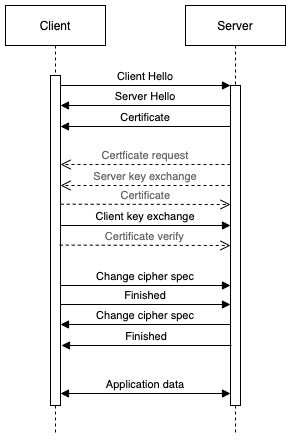
\includegraphics[scale=0.7]{img/tls.png}}
% otherwise see the example in the following (commented out) line
% to scale it 50% (e.g. 20pt font get scaled to 10pt font)
%   \centerline{\includegraphics[scale=0.5]
% if you have a picture (i.e. no text hence no font size problem)
% you can fit it relatively to the page width
%   \centerline{\includegraphics[width=0.9\textwidth]
\caption{TLS handshake between a client and a server.}
\label{fig:tls}
\end{figure}

In \myfig{\ref{fig:tls}} an example of a typical TLS handshake is shown. The dashed arrows in the figure correspond to optional messages.
The TLS handshake starts after the creation of a TCP connection between client and server through the TCP handshake.

First, the client sends a ``Client Hello" message, which includes the desired TLS version, a list of cipher suites, a random number and a list of compression methods. The server replies with a ``Server Hello" containing a random number and the mutually supported TLS version, the chosen cipher suite and the chosen compression method. A cipher suite specifies an encryption algorithm, a key exchange mechanism and a hash algorithm, useful for integrity purposes.
For the sake of simplicity, we can refer to this first part of the TLS handshake as the cipher suite negotiation phase. These two initial messages can also be enriched with additional information, through TLS extensions.

Later, just the server authentication or a peer authentication - both for the client and for the server - can happen. This can be referred to as the authentication phase, and it is realised through SSL/TLS certificates.

These are digital certificates following X.509 standard for certificates. Broadly, a X.509 certificate contains the certificate itself (with various information including the certification authorities involved in the certificate, the subject name of the owner of the certificate and its public key), an identifier of the signature algorithm used to sign the certificate and the signature of the certificate.

The server sends its certificate containing its public key and undergoes an asymmetric implicit challenge. If also the client authentication is required, the server sends a ``Certificate request". Then the client, analogously, sends its public key with a certificate and undergoes an explicit challenge.

Once the authentication phase is completed\footnote{The ``Server key exchange" and the ``Certificate verify" messages are optional and used only in specific contexts.}, the key agreement phase can start. The client computes a pre-master secret, encrypts it with the public key of the server and sends it through the ``Client key exchange" message. Then, both client and server compute a master secret using the pre-master secret and the random numbers exchanged previously. In this way the client and server can communicate using a shared symmetric key, obtained from the master secret.

Then, in the final phase, the ``Change cipher spec" messages activate the protection respectively on each sender side. 
At last, the ``Finished" message is used for security purposes, as it contains the MAC of all previous messages. This message is the first one to be encrypted: from now on all messages will be protected by the negotiated algorithms.

This is a typical TLS handshake procedure. In the following section, we will highlight the steps in which the SPHINCS+ algorithm will play a role.

\subsection{SPHINCS+ integration}
\label{sub:integration}

The integration of post-quantum cryptography in network protocols is composed by several steps.

Each network protocol first must be evaluated to search for constraints that could potentially make challenging the addition of new algorithms. This is the case when protocols were not designed to replace or negotiate cryptographic algorithms, or when strict limitations on sizes of keys or packets are present \cite{6_NISTPQC_TLS_SSH}.
The next step consists in deciding how to integrate the new algorithm. This concerns for example decisions about how parameters and keys should be represented in the network packets.
Moreover, all these design choices must be done in a way that preserves backward compatibility with the endpoints that have not yet been upgraded \cite{6_NISTPQC_TLS_SSH}.

In this chapter, we focus on the TLS network protocol. 
Starting from the previous TLS protocol overview, in this section we are going to describe how a post-quantum authentication mechanism, such as SPHINCS+, plays a role in the entire workflow of the TLS handshake.
Since SPHINCS+ is mainly involved during the authentication phase, later we will deepen that specific phase, describing which modifications to the original implementation have been done.

\subsubsection{Workflow}

As depicted before, the TLS handshake workflow is composed of the cipher suite negotiation phase, the authentication phase, the key agreement phase and the final phase\footnote{Note that these names of phases are not standard, but they have been introduced for the reader, in order to provide a clearer explanation.}.

From now on we will consider a classic web scenario in which the client is not authenticated: the authentication phase comprehends only the server authentication, done with X.509 certificates. For what concerns the client authentication, the considerations would be the same as the ones for the server authentication.

In TLS, digital signatures are used during the authentication phase in order to authenticate the parties. Then, during the key agreement phase, a key exchange mechanism is used to establish a shared secret, which can then be used in symmetric cryptography.
This means that, for security against a future quantum adversary, we should incorporate post-quantum authentication and post-quantum key exchange in those phases.

The post-quantum key exchange is necessary since an adversary who can discover the symmetric key would break the confidentiality of all the TLS records \cite{10_postquantum_keyexchange}. Breaking the authentication phase instead could enable the attacker to send malicious certificates, impersonating the server and performing a MITM attack.

Now, we focus on the TLS handshake with post-quantum authentication algorithms, analysing it phase by phase:

\begin{enumerate}
    \item \textit{Cipher suite negotiation phase}. Referring to the TLS handshake in \myfig{\ref{fig:tls}}, the first message to take into consideration is the ``Client Hello" message. This message will negotiate the desired post-quantum signature algorithm exploiting the TLS extension for specifying signature algorithms \cite{5_postquantum_signature_usecase}. This works in the same way also for the ``Server Hello" message;
    \item \textit{Authentication phase}. In the successive phase the server will send its certificate or its chain of certificates. These certificates will now include post-quantum certificates.
    In order to implement post-quantum authentication, new Algorithm Identifiers for X.509 need to be added \cite{5_postquantum_signature_usecase}.
    Each Algorithm Identifier uniquely identifies a cryptographic algorithm inside a certificate.
    Thus, a post-quantum certificate will have the post-quantum public key of the subject and the specific post-quantum signature algorithm used to create that signature \cite{5_postquantum_signature_usecase}.
    This certificate will be signed by the issuer using his post-quantum private key. The post-quantum signature will be appended in a specific field of the certificate, the ``Signature" one.
    As exposed in \cite{5_postquantum_signature_usecase}, the addition of the post-quantum public key and signature to the SSL certificate will increase the size of the single certificate, hence also the size of the certificate chain will increase.
    This is not a problem since, as it happens normally in TLS, when a certificate chain exceeds a certain length, of 16 KB, TLS will exploit the fragmentation of records to split packets before sending them.
    \item \textit{Key agreement phase}. After the authentication phase, the key agreement is performed.
    The key agreement phase will be the same as before, using standard cryptography. If post-quantum key exchange mechanism are needed, the ``Client key exchange" message will be using the PQ key exchange defined into the cipher suites of the ``Client Hello" and ``Server Hello" messages.
    \item \textit{Certificate verify from server}. This is a new step with respect to the standard TLS handshake protocol. In addition to the standard schema, the server will also sign the transcripts of the handshake. It will transmit a post-quantum ``Certificate verify" message, which contains a PQ signature which the client will verify along with the signatures in the certificate chain \cite{5_postquantum_signature_usecase}.
    \item \textit{Final phase}. Eventually, the final phase works as for the standard TLS handshake schema.
\end{enumerate}

Since the most affected part of the schema is the authentication phase, in the following section we will focus on how the messages and certificates involved in this part are going to be enhanced.

\subsubsection{Authentication phase}

In this section we present the needed modifications to the TLS protocol in order to implement post-quantum authentication. All the modifications presented here refer to the OpenSSL fork from post-quantum algorithm made by the Open Quantum Safe project. We will discuss about this project in Section \ref{sub:openquantumsafeproject}. 

In order to practically implement these modifications both for post-quantum key exchange and authentication mechanisms, some failures occurred because of large message sizes \cite{6_NISTPQC_TLS_SSH}: for key exchange mechanisms this was due to large public keys or ciphertexts; for signature algorithms those large sizes were due to large public keys or large signatures.

Some of these failures involved sizes bigger than the ones of the protocol specification. To fix them, a solution could be possible to change the protocol specification, as for example increasing when needed the maximum length of fields inside messages. Unfortunately, this solution would increase the risk of incompatibility with existing implementations. This situation happens in the case of some PQ algorithms, such as most of the Picnic signature scheme variants. This was not the case of the SPHINCS+ signature scheme.

Other failures, instead, involved sizes that were within protocol specification tolerances, but where its implementation originally has parameters or internal buffers set smaller than the maximum size allowed by the specification.
In these cases, the work done by \cite{6_NISTPQC_TLS_SSH} was to increase the implemented buffer lengths or the sizes of parameters, in order to make the algorithm fit: this was the solution exploited to implement most of the SPHINCS+ variants inside OpenSSL.

Referring specifically to post-quantum authentication, it is important to recall that in TLS 1.3 the maximum X.509 certificate size is $2^{24} - 1$ bytes. Moreover, the maximum signature size - used in the ``Certificate Verify" message - is of $2^{16} - 1$ bytes.
However, the OpenSSL implementation of the TLS 1.3 protocol adds some extra constraints.

First, it limits the default maximum size of the ``Certificate" message, which includes the chain of all SSL certificates except for the root, to $102400$ bytes. Most of post-quantum signature schemes can work with this size, except for some implementations of the Rainbow signature scheme. This value was raised to $2^{24} - 1$ bytes allowing also the remaining Rainbow schemes to work \cite{6_NISTPQC_TLS_SSH}.

For what concerns the signature inside the ``Certificate verify" message, its maximum size is set to $2^{14}$ bytes.
Since this value is too small for many post-quantum signatures, including all SPHINCS+ variants except one, this maximum size was raised to $2^{16} - 1$ \cite{6_NISTPQC_TLS_SSH}, thus allowing all SPHINCS+ variants to work.

Finally, we highlight an important concept. In the real-world transition from standard authentication algorithms and post-quantum ones it is necessary to provide implementations that support both standard and post-quantum authentication algorithms, since post-quantum algorithms would be less mature and less used during this period. These implementations must also be backwards compatible with those implementations that have not yet been upgraded during the transition.

\subsection{Open Quantum Safe project}
\label{sub:openquantumsafeproject}

In order to have the possibility to test post-quantum algorithms inside real case scenarios, the IETF started the Open Quantum Safe project in 2016, an open-source software project.
The Open Quantum Safe (OQS) project\footnote{\url{https://openquantumsafe.org}} aims to develop and prototype quantum-resistant cryptography, integrating post-quantum schemes in the liboqs library.

\textit{liboqs} is an open source C library projected by Douglas Stebila and Michele Mosca. It provides implementations of post-quantum cryptographic algorithms in order to facilitate the deployment and testing of them in real word scenarios. The library is realised using a common interface which is based on the implementations from NIST submission packages \cite{16_Quantum}.
Initially, liboqs focused solely on key exchange algorithms and then expanded also to signature algorithms. liboqs provides a common API for post-quantum key exchange and signatures algorithms. It includes also a test harness and benchmarking routines to compare performance of post-quantum implementations against standard cryptographic algorithms.

Moreover, in order to complete the integration of PQC inside TLS, OQS provides integration of the liboqs library inside OpenSSL, creating a fork specific for post-quantum algorithms. This fork\footnote{\url{https://github.com/open-quantum-safe/openssl}} is a fork of OpenSSL 1.1.1 which adds post-quantum key exchange and authentication algorithms using liboqs to TLS 1.3, for prototyping and evaluation purposes.

Ever since a new scheme is proposed to a NIST submission, it is first prototyped inside liboqs. Once in there, the scheme is enabled in the OpenSSL fork \cite{16_Quantum}.

The strength of the OpenSSL post-quantum integration is that it can have ``generic" ciphersuites and signature algorithms.
There are two ways in which OpenSSL can use a certain key exchange or signature mechanism \cite{10_postquantum_keyexchange}:
\begin{enumerate}
    \item Runtime: liboqs includes interfaces for each key exchange and signature algorithm so it can be selected by the caller at runtime;
    \item Compile time: liboqs also includes a generic interface that can be configured at compile time.
\end{enumerate}

In the latter mode, the ``generic" key exchange or signature methods can be hard-coded at compile time to any of the available implementations. The OpenSSL fork already includes both a ``generic OQS key exchange" mechanism and a ``generic OQS signature" algorithm, that respectively call the ``liboqs generic key exchange" or the ``liboqs generic signature" methods.


\subsection{Testing}
\label{sub:testing}

In this section we present tests for the SPHINCS+ signature scheme. First we describe our testbed. The testbed is divided in two main parts: the one related to the performance of the single algorithms and the one related to the performance of the TLS handshake performed with these algorithms. The testbed will be described in the next section.
In the two subsequent sections, both results will be presented.
For the first part, all SPHINCS+ variants have been evaluated measuring their sign and verify times. 
These values will be compared to RSA2048 and ECDSA384 values.
Finally, in this first part the most known post-quantum key exchange algorithms have been evaluated in order to evaluate the fastest one. This step will be useful for comparing a TLS handshake performed with standard cryptography against a totally post-quantum TLS handshake.

In the second part of the testbed, we evaluated the performances of post-quantum signature algorithms, integrated into TLS 1.3 using OpenSSL 1.1.1. This was done observing the number of TLS connections established per second. These values will be computed using as signature algorithms all SPHINCS+ variants, plus standard RSA and ECDSA algorithms. 

Then, in Section \ref{subsub:comparison}
we will make some observations about the retrieved data.

\subsubsection{Testbed design}
% Describe: general purpose of the experiments (functional evaluation, performance evaluation, comparison with other stuff), experimental setup (hardware and software, including detailed build and configuration instructions if needed)

The testbed developed during this work aims to test the SPHINCS+ framework inside the TLS context.
First, SPHINCS+ along with all its variants is tested and compared to standard signature schemes: RSA and ECDSA. This is done exploiting the liboqs test suite library.
Second, SPHINCS+ is used as the signature algorithm in the authentication phase of the TLS handshake procedure. The performance of TLS handshakes made with SPHINCS+ are compared to TLS handshakes performed with standard signature algorithms.

The software experimental setup is composed by 9 bash scripts, that can be run by command line directly. They can be divided into ``build", ``run" and ``clean" scripts. Scripts referring to the first part of the testbed, the one concerning the testing of SPHINCS+ signature schemes, are identified by the ``testbed\_liboqs" keywords. Scripts referring to testing the SPHINCS+ integration inside TLS are identified just by the ``testbed" keyword.

Concerning the hardware setup, all the experiments involved a computer equipped with 16GB of RAM, a CPU Intel i7-8550U with 4 cores of 1.80 GHz each. All tests were running Ubuntu 18.04.5 LTS on a 64-bit architecture.

% Then describe each experiment: its specific purpose (\eg\ testing a specific feature of the protocol), the command run, and the output (expected and actual). You can use a table like \mytab{\ref{tab:results}} to group the results (for example if the same experiment was repeated with several data sizes)

We can now describe in details our testbed. The testbed is divided into two main parts: ``liboqs" and ``openssl".

The ``liboqs" part focuses on the performance evaluation of SPHINCS+. This is done computing the times for the sign and verify operations of the SPHINCS+ variants, compared to the times of RSA and ECDSA signature algorithms. In this part, also the most common post-quantum key exchange mechanisms are evaluated in this test suite in order to select the fastest one. The fastest key exchange mechanism will be used in the second part of the testbed for establishing TLS connections.
This part contains the following bash scripts:
\begin{itemize}
    \item \textit{build\_testbed\_liboqs.sh} downloads both liboqs and OpenSSL libraries inside an ad-hoc  directory, ``testbed\_for\_liboqs\_tests", and builds them. The liboqs is compiled to have as default signature algorithm SPHINCS+-Haraka-128f-robust. This signature algorithm is then used to create a public and private key pair and to issue X.509 certificates. This step is performed in order to enable the library to be used when necessary.
    The reason why also the OpenSSL library is installed in this first part is that standard cryptographic algorithms can not be tested through the liboqs test suite, so the OpenSSL test suite need to be used (for RSA and ECDSA).
    \item \textit{run\_testbed\_liboqs.sh} runs the test suites provided by the liboqs library for post-quantum algorithms. All SPHINCS+ variants are tested with the ``test\_sig" script of liboqs. Moreover, post-quantum key exchange algorithms like BIKE, Frodo and NTRU are tested with the ``test\_kem" script inside liboqs. These algorithms are evaluated in order to find the most efficient one, which will be used inside the ``openssl" part for evaluating the performance of a TLS handshake performed with both post-quantum signature and key exchange algorithms.
    \item \textit{run\_testbed\_liboqs\_rsaecdsa.sh}  runs multiple times (10) the ``openssl speed" command for evaluating the performance of RSA2048 and ECDSA384 algorithms. The command is executed multiple times in order to be able to compute the mean and the standard deviation of the obtained values.
    \item \textit{clean\_testbed\_liboqs.sh} deletes the ``testbed\_for\_liboqs\_tests" directory.
\end{itemize}

Then, the second part of the testbed is the ``openssl" one. The ``openssl" part then is the most important part of our testbed, since it focuses on the performance evaluation of SPHINCS+ inside the OpenSSL library. This part contains the following bash scripts:
\begin{itemize}
    \item \textit{\textbf{build\_testbed.sh}} is the most important script in the testbed of this work. First, it iterates on the list of all SPHINCS+ variants (36). It compiles the liboqs library with the current variant set as the default signature algorithm. Then, both the liboqs and OpenSSL libraries are built. It then calls the ``run\_testbed.sh" script, passing to it as parameter the current SPHINCS+ variant.
    If the memory of the current machine is not enough to support multiple installations of the liboqs and OpenSSL libraries, it finally calls the ``clean\_testbed.sh" script. This setting is the default one, but it can be statically changed inside the script.
    The liboqs and OpenSSL libraries have to be rebuilt for each SPHINCS+ variant. This is necessary since the implementation of SPHINCS+ into OpenSSL is not available yet. The only way to test it into the TLS scenario is to compile the liboqs library with SPHINCS+ as the default signature algorithm, and then use the OpenSSL library to perform TLS handshakes with the default signature algorithm of the liboqs library.
    \item \textit{build\_testbed\_single\_variant.sh} is a support script which enables to build the liboqs and OpenSSL libraries. The default signature algorithm can be specified with this script by command line as first parameter. The algorithm has to be specified in the form ``OQS\_SIG\_alg\_sphincs\_haraka\_128f\_robust".
    \item \textit{run\_testbed.sh} tests a single SPHINCS+ variant, passed as first parameter by command line. It launches a TLS server and evaluates the performance of the TLS handshake with the ``s\_time" command, multiple times (10). For each SPHINCS+ variant, the TLS handshake is performed with two times: with the Diffie-Hellman key exchange and with the NTRU hps2048509 post-quantum key exchange algorithm. This is the most efficient post-quantum key exchange algorithm among the ones tested by the ``run\_testbed\_liboqs.sh" script.
    \item \textit{run\_testbed\_rsaecdsa.sh} evaluates the performances of TLS handshakes performed with RSA2048 and ECDSA384 signature algorithms.
    For each signature algorithm, it creates inside the OpenSSL library the respective key pairs and X.509 certificates, and then iterates multiple times (10) executing the ``s\_time" command.
    \item \textit{clean\_testbed.sh} deletes the ``testbed" directory.
\end{itemize}

All of those scripts are contained inside the ``tests" directory, which must be installed inside home directory. All outputs results are written into the ``results" directory, which is contained inside the ``tests" directory.
All files related to the first part of the testbed, the ``liboqs" part, are in the format ``output\_liboqs\_*.txt".
All files related to the second part of the testbed, the one focusing on TLS integration, are in the format ``output\_tls\_s\_time\_*.txt".

The output files produced are the following ones:
\begin{itemize}
    \item \textit{output\_liboqs\_kem.txt} contains the performance values for encapsulating and decapsulating keys for post-quantum key exchange algorithms: BIKE, Frodo and NTRU with all their respective variants.
    \item \textit{output\_liboqs\_sig.txt} contains the performance values for the key generation, sign and verify operations for post-quantum authentication mechanisms: SPHINCS+ with all its variants.
    \item \textit{output\_liboqs\_std\_sig.txt} contains the performance values for sign and verify operations for standard signature algorithms: RSA2048 and ECDSA384. These two were chosen since they are the currently most used signature algorithms in TLS handshakes.
    \item \textit{output\_tls\_s\_time.txt} contains the statistics for TLS handshakes performed with SPHINCS+ as the signature algorithm inside the authentication phase of the handshake. For each SPHINCS+ variant, the handshake is performed with DH and NTRU key exchange mechanisms.
    \item \textit{output\_tls\_s\_time\_rsaecdsa.txt} contains the statistics for TLS handshakes performed with RSA2048 and ECDSA384 as the signature algorithms inside the authentication phase of the handshake.
\end{itemize}

Additional information about the testbed can be found in the User manual in Section \ref{sec:usermanual}, in the Programmer manual in Section \ref{sec:programmermanual} and in the documentation of our code\footnote{\url{https://git-sec.polito.it/post-quantum-crypto/sphincs-tls}}.

The results obtained running this testbed are presented in the following Section \ref{subsub:perf_liboqs} and \ref{subsub:perf_openssl}.

\subsubsection{Performances on liboqs}
\label{subsub:perf_liboqs}

In this section, data about performances of the SPHINCS+ framework are presented.

In \mytab{\ref{tab:results_sig_liboqs}}, times of ``sign" and ``verify" operations of RSA2048, ECDSA384 and all the SPHINCS+ variants are shown. Looking at the table we can notice that all SPHINCS+ variants take at least ten times the time taken by RSA2048 to perform a ``sign" or a ```verify" operation. 

\begin{table}[]
\centering
\begin{tabular}{@{}lrrrr@{}}
\toprule
\textbf{Signature algorithm}  & \multicolumn{2}{c}{\textbf{Sign ($ms$)}} & \multicolumn{2}{c}{\textbf{Verify ($ms$)}}        \\ \midrule
                              & \multicolumn{1}{c}{\textit{Mean}}               & \multicolumn{1}{c}{\textit{St. Dev.}}  & \multicolumn{1}{c}{\textit{Mean}}        & \multicolumn{1}{c}{\textit{St. Dev.}} \\ \hline
RSA-2048-SHA256      & 0.53 & 0.03 & 0.02 & 0.00 \\
ECDSA-nistp384-SHA256 & 1.01  & 0.12  & 0.87  & 0.07          \\ \hline
SPHINCS+-Haraka-128f-robust & 11.30   & 1.01  & 0.46 & 0.05 \\
SPHINCS+-Haraka-128f-simple & 6.88   & 0.31  & 0.29 & 0.03 \\
SPHINCS+-Haraka-128s-robust & 176.61 & 2.46  & 0.19 & 0.02 \\
SPHINCS+-Haraka-128s-simple & 173.72 & 9.65  & 0.18 & 0.03 \\
SPHINCS+-Haraka-192f-robust & 12.66  & 0.55  & 0.72 & 0.07 \\
SPHINCS+-Haraka-192f-simple & 9.54   & 0.66  & 0.48 & 0.06 \\
SPHINCS+-Haraka-192s-robust & 349.40  & 4.42  & 0.28 & 0.04 \\
SPHINCS+-Haraka-192s-simple & 297.05 & 5.62  & 0.19 & 0.02 \\
SPHINCS+-Haraka-256f-robust & 27.67  & 1.44  & 0.67 & 0.07 \\
SPHINCS+-Haraka-256f-simple & 25.76  & 1.33  & 0.57 & 0.06 \\
SPHINCS+-Haraka-256s-robust & 270.80  & 31.97 & 0.38 & 0.05 \\
SPHINCS+-Haraka-256s-simple & 194.72 & 2.60   & 0.27 & 0.03 \\ \hline
SPHINCS+-SHA256-128f-robust & 28.50    & 1.01  & 3.80  & 0.36 \\
SPHINCS+-SHA256-128f-simple & 15.77   & 0.36  & 1.96 & 0.15 \\
SPHINCS+-SHA256-128s-robust & 487.24  & 9.51  & 1.53 & 0.12 \\
SPHINCS+-SHA256-128s-simple & 275.15  & 4.94  & 0.81 & 0.09 \\
SPHINCS+-SHA256-192f-robust & 39.56   & 0.82  & 6.21 & 0.42 \\
SPHINCS+-SHA256-192f-simple & 22.55   & 1.09  & 3.13 & 0.25 \\
SPHINCS+-SHA256-192s-robust & 931.96  & 13.37 & 2.37 & 0.22 \\
SPHINCS+-SHA256-192s-simple & 534.15  & 11.70  & 1.26 & 0.13 \\
SPHINCS+-SHA256-256f-robust & 140.13  & 2.99  & 7.85 & 0.44 \\
SPHINCS+-SHA256-256f-simple & 46.74   & 1.43  & 3.08 & 0.19 \\
SPHINCS+-SHA256-256s-robust & 1090.82 & 4.59  & 3.99 & 0.13 \\
SPHINCS+-SHA256-256s-simple & 341.20   & 1.36  & 1.51 & 0.11 \\ \hline
SPHINCS+-SHAKE256-128f-robust & 74.27   & 1.58  & 5.67 & 0.38 \\
SPHINCS+-SHAKE256-128f-simple & 40.99   & 0.74  & 2.89 & 0.20  \\
SPHINCS+-SHAKE256-128s-robust & 1096.19 & 3.39  & 2.24 & 0.12 \\
SPHINCS+-SHAKE256-128s-simple & 666.51  & 1.79  & 1.25 & 0.11 \\
SPHINCS+-SHAKE256-192f-robust & 94.79   & 0.82  & 8.83 & 0.30  \\
SPHINCS+-SHAKE256-192f-simple & 53.95   & 0.99  & 4.92 & 0.28 \\
SPHINCS+-SHAKE256-192s-robust & 2261.57 & 0.00     & 3.45 & 0.19 \\
SPHINCS+-SHAKE256-192s-simple & 1403.38 & 31.19 & 1.83 & 0.19 \\
SPHINCS+-SHAKE256-256f-robust & 198.78  & 2.60   & 9.29 & 0.38 \\
SPHINCS+-SHAKE256-256f-simple & 110.82  & 1.48  & 4.79 & 0.17 \\
SPHINCS+-SHAKE256-256s-robust & 1605.04 & 0.00     & 4.59 & 0.17 \\
SPHINCS+-SHAKE256-256s-simple & 935.14  & 3.56  & 2.33 & 0.17 \\ \bottomrule
\end{tabular}
\caption{Performances of Sign and Verify operations for RSA2048, ECDSA384 and SPHINCS+ signature algorithms. The time to perform these operations is expressed in $ms$.}
\label{tab:results_sig_liboqs}
\end{table}


For what concerns post-quantum key exchange performances, in \mytab{\ref{tab:results_kem_liboqs}} statistics are presented. From this table it is possible to notice that among the chosen algorithms, the most efficient is NTRU-HPS-2048-509. This is the third fastest algorithm for the ``encaps" operation and the fastest one for the ```decaps" operation. This will be the algorithm used as key exchange mechanism for establishing TLS connections in the second part of our testbed.


\begin{table}[]
\centering
\begin{tabular}{@{}lrrrr@{}}
\toprule
\textbf{Key Exchange algorithm} & \multicolumn{2}{c}{\textbf{Encaps ($ms$)}}         & \multicolumn{2}{c}{\textbf{Decaps ($ms$)}}                        \\ \midrule
                                & \multicolumn{1}{c}{\textit{Mean}} & \multicolumn{1}{c}{\textit{St. Dev.}} & \multicolumn{1}{c}{\textit{Mean}} & \multicolumn{1}{c}{\textit{St. Dev.}} \\ \hline
FrodoKEM-640-AES    & 0.63 & 0.04 & 0.61 & 0.03 \\
FrodoKEM-640-SHAKE  & 2.37 & 0.13 & 2.43 & 0.12 \\
FrodoKEM-976-AES    & 1.29 & 0.06 & 1.24 & 0.05 \\
FrodoKEM-976-SHAKE  & 5.34 & 0.28 & 5.35 & 0.31 \\
FrodoKEM-1344-AES   & 2.27 & 0.08 & 2.24 & 0.09 \\
FrodoKEM-1344-SHAKE & 9.49 & 0.49 & 9.50  & 0.47  \\ \hline
NTRU-HPS-2048-509 & 0.19 & 0.02 & 0.48 & 0.03 \\
NTRU-HPS-2048-677 & 0.32 & 0.03 & 0.85 & 0.06 \\
NTRU-HPS-4096-821 & 0.44 & 0.04 & 1.21 & 0.08 \\
NTRU-HRSS-701     & 0.31 & 0.03 & 0.90  & 0.07   \\ \hline
BIKE1-L1-CPA & 0.11 & 0.01 & 1.36 & 0.04 \\
BIKE1-L3-CPA & 0.35 & 0.03 & 5.13 & 0.16 \\
BIKE1-L1-FO  & 0.15 & 0.01 & 1.82 & 0.07 \\
BIKE1-L3-FO  & 0.50  & 0.02 & 6.83 & 0.37   \\ \bottomrule
\end{tabular}
\caption{Performances of Encaps and Decaps operations for Frodo, NTRU and BIKE key exchange algorithms. The time to perform these operations is expressed in $ms$.}
\label{tab:results_kem_liboqs}
\end{table}


\subsubsection{Performances on OpenSSL}
\label{subsub:perf_openssl}

In this section, data about performances of TLS 1.3 handshakes with SPHINCS+ integration are presented.

In \mytab{\ref{tab:results_s_time}}, the number of connections established per user per second is shown for each combinations of algorithms. First, classical TLS handshake performances are presented, with DH key exchange combined with both RSA2048 and ECDSA384 signature algorithms. Then, post-quantum handshake performances are provided for each SPHINCS+ variant. Each SPHINCS+ variant is used in combination with DH and post-quantum NTRU key exchange mechanisms. 

\begin{table}[]
\centering
\begin{tabular}{@{}lrrrr@{}}
\toprule
\textbf{Signature algorithm}  & \multicolumn{2}{c}{\textbf{Diffie-Hellman}} &  \multicolumn{2}{c}{\textbf{NTRU}} \\ \midrule
                            & \multicolumn{1}{c}{\textit{Mean}}           & \multicolumn{1}{c}{\textit{St. Dev.}} & \multicolumn{1}{c}{\textit{Mean}}             & \multicolumn{1}{c}{\textit{St. Dev.}} \\ \hline
RSA-2048-SHA256                     & 3179                                    & 134                        & \multicolumn{1}{c}{-}                         & \multicolumn{1}{c}{-}                 \\
ECDSA-nistp384-SHA256                     & 794                                     & 34                         & \multicolumn{1}{c}{-}                         & \multicolumn{1}{c}{-}                 \\ \hline
SPHINCS+-Haraka-128f-robust   & 907                                      & 29                         & 167                                       & 1                          \\
SPHINCS+-Haraka-128f-simple   & 1099                                    & 17                         & 172                                       & 1                        \\
SPHINCS+-Haraka-128s-robust   & 1400                                    & 200                        & 162                                       & 7                          \\
SPHINCS+-Haraka-128s-simple   & 1638                                    & 358                        & 186                                       & 6                          \\
SPHINCS+-Haraka-192f-robust   & 651                                     & 22                         & 159                                       & 3                          \\
SPHINCS+-Haraka-192f-simple   & 813                                     & 29                         & 164                                       & 3                          \\
SPHINCS+-Haraka-192s-robust   & 1496                                    & 553                        & 177                                       & 7                         \\
SPHINCS+-Haraka-192s-simple   & 2041                                    & 1076                       & 175                                       & 12                         \\
SPHINCS+-Haraka-256f-robust   & 663                                     & 28                       & 161                                       & 5                         \\
SPHINCS+-Haraka-256f-simple   & 719                                      & 21                         & 165                                       & 5                          \\
SPHINCS+-Haraka-256s-robust   & 1003                                      & 226                       & 175                                       & 5                         \\
SPHINCS+-Haraka-256s-simple   & 1192                                    & 275                        & 178                                       & 10                         \\ \hline
SPHINCS+-SHA256-128f-robust   & 221                                     & 7                        & 112                                       & 2                         \\
SPHINCS+-SHA256-128f-simple   & 383                                     & 10                        & 137                                       & 4                       \\
SPHINCS+-SHA256-128s-robust   & 500                                         & 48                        & 141                                       & 6                          \\
SPHINCS+-SHA256-128s-simple   & 849                                         & 155                        & 161                                       & 7                         \\
SPHINCS+-SHA256-192f-robust   & 142                                     & 4                          & 84                                        & 2                       \\
SPHINCS+-SHA256-192f-simple   & 248                                     & 9                          & 115                                       & 3                         \\
SPHINCS+-SHA256-192s-robust   & 407                                     & 114                        & 127                                       & 15                        \\
SPHINCS+-SHA256-192s-simple   & 549                                     & 82                        & 149                                       & 6                          \\
SPHINCS+-SHA256-256f-robust   & 111                                     & 5                        & 72                                        & 2                          \\
SPHINCS+-SHA256-256f-simple   & 246                                     & 8                         & 113                                       & 3                        \\
SPHINCS+-SHA256-256s-robust   & 209                                         & 24                        & 98                                        & 11                        \\
SPHINCS+-SHA256-256s-simple   & 454                                     & 40                        & 147                                       & 9                         \\ \hline
SPHINCS+-SHAKE256-128f-robust & 143                                     & 4                          & 86                                        & 3                        \\
SPHINCS+-SHAKE256-128f-simple & 253                                     & 9                         & 115                                        & 3                          \\
SPHINCS+-SHAKE256-128s-robust & 319                                     & 70                         & 112                                       & 9                       \\
SPHINCS+-SHAKE256-128s-simple & 525                                         & 80                        & 142                                       & 8                         \\
SPHINCS+-SHAKE256-192f-robust & 94                                      & 3                          & 65                                        & 1                         \\
SPHINCS+-SHAKE256-192f-simple & 164                                    & 5                          & 94                                        & 3                       \\
SPHINCS+-SHAKE256-192s-robust & 245                                        & 15                         & 97                                        & 12                         \\
SPHINCS+-SHAKE256-192s-simple & 495                                         & 190                        & 125                                       & 12                        \\
SPHINCS+-SHAKE256-256f-robust & 84                                      & 9                          & 62                                        & 3                          \\
SPHINCS+-SHAKE256-256f-simple & 165                                     & 8                         & 93                                        & 3                          \\
SPHINCS+-SHAKE256-256s-robust & 185                                     & 22                        & 88                                        & 6                          \\
SPHINCS+-SHAKE256-256s-simple & 360                                     & 76                         & 116                                       & 8                          \\ \bottomrule
\end{tabular}
\caption{Number of connections established per user per second for Diffie-Hellman and NTRU hps2048509 key exchange algorithms, for RSA2048, ECDSA384 and SPHINCS+ signatures schemes.}
\label{tab:results_s_time}
\end{table}

\subsubsection{Comparison}
\label{subsub:comparison}

%liboqs results
Analysing the results obtained in the previous sections, we can provide some graphs in order to make observations about data.

In \myfig{\ref{fig:chartSV}}, the performance of SPHINCS+ signature algorithms are grouped together by parameter values and compared to RSA and ECDSA performances. The time necessary for performing a ``sign" or a ``verify" operation with SPHINCS+ is greater than the one for RSA and ECDSA operations.
Besides, also the different underlying hash function has a significant impact on the duration of these operations. In general, the SPHINCS+ variants exploiting the Haraka hash functions are much more faster than SHA256 and SHAKE256 variants. The latter one makes the slowest SPHINCS+ variants.

The huge overhead introduced by most of the SPHINCS+ variants with respect to RSA2048, as mentioned in \cite{8_ARM}, may be acceptable for non-interactive applications, when there is the need for long term security and for stateless schemes. For what concerns instead interactive applications, like the TLS protocol, probably further algorithmic improvements to these schemes would enable deployment on a broader scale. For now, the overhead in 
``sign" and ``verify" operations would heavily impact the establishment of TLS connections, as showed by the next analysis on the results of the second part of our testbed.

Now we can briefly focus on post-quantum key exchange algorithms.
Remarking the considerations made previously in Section \ref{subsub:perf_liboqs}, the performances of post-quantum key exchanges are represented in \myfig{\ref{fig:chartED}}. From these charts it is possible to confirm our statements about the NTRU-HPS-2048-509 algorithm. This is the third fastest algorithm for encapsulation operations and the first one for decapsulation operations. 
Moreover, this NTRU variant takes the least amount of time for performing these two operations one after the other.
Other algorithms that are fast for the encapsulation phase, as for example BIKE1-L1-CPA and BIKE1-L1-FO, are not among the fastest ones globally, since the decapsulation phase takes a significant amount of time.
For these reasons, we selected the NTRU-HPS-2048-509 algorithm as the key exchange mechanism for TLS handshakes.

\begin{figure}
\centering
% If the picture uses fonts of the correct size (10 ... 12 pt)
% then it can be included without scaling
\centerline{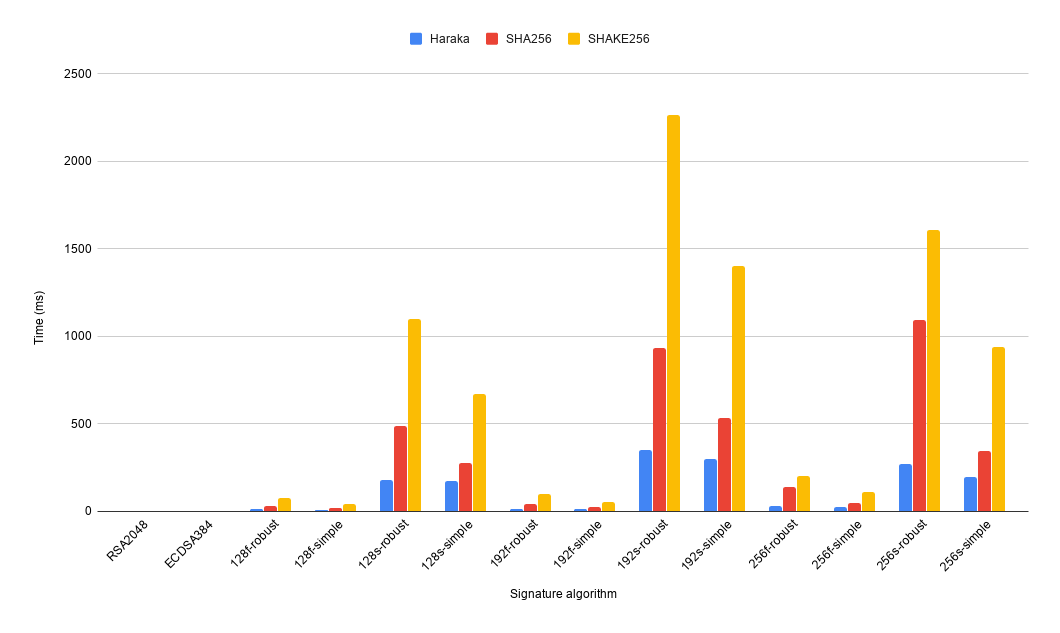
\includegraphics[scale=0.48]{tesina_SPHINCS/img/chartSign.png}}
\centerline{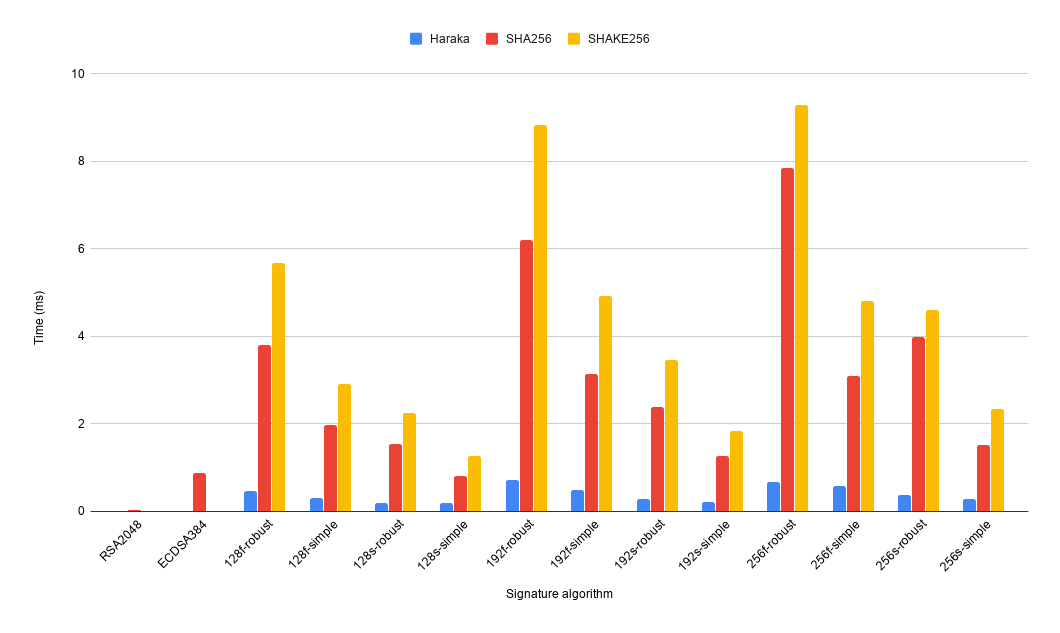
\includegraphics[scale=0.48]{tesina_SPHINCS/img/chartVerify.png}}
% otherwise see the example in the following (commented out) line
% to scale it 50% (e.g. 20pt font get scaled to 10pt font)
%   \centerline{\includegraphics[scale=0.5]
% if you have a picture (i.e. no text hence no font size problem)
% you can fit it relatively to the page width
%   \centerline{\includegraphics[width=0.9\textwidth]
\caption{Times for performing Sign and Verify operations of signature schemes. On the top chart, Sign times in $ms$ are shown, while on the bottom chart, Verify times in $ms$ are shown.}
\label{fig:chartSV}
\end{figure}

\begin{figure}
\centering
% If the picture uses fonts of the correct size (10 ... 12 pt)
% then it can be included without scaling
\centerline{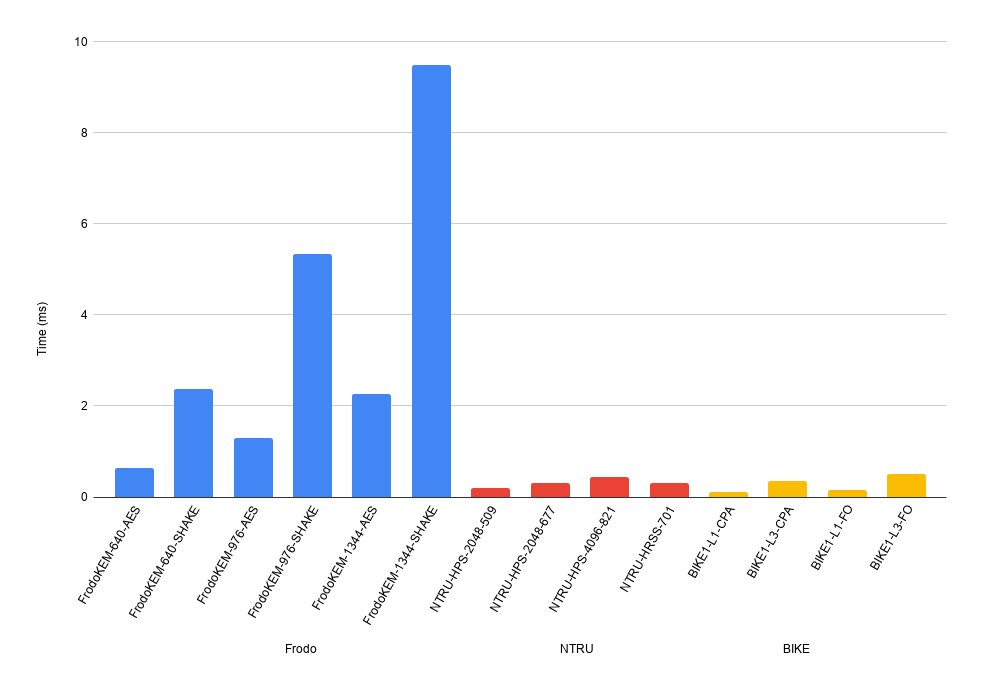
\includegraphics[scale=0.5]{tesina_SPHINCS/img/chartEncaps.png}}
\centerline{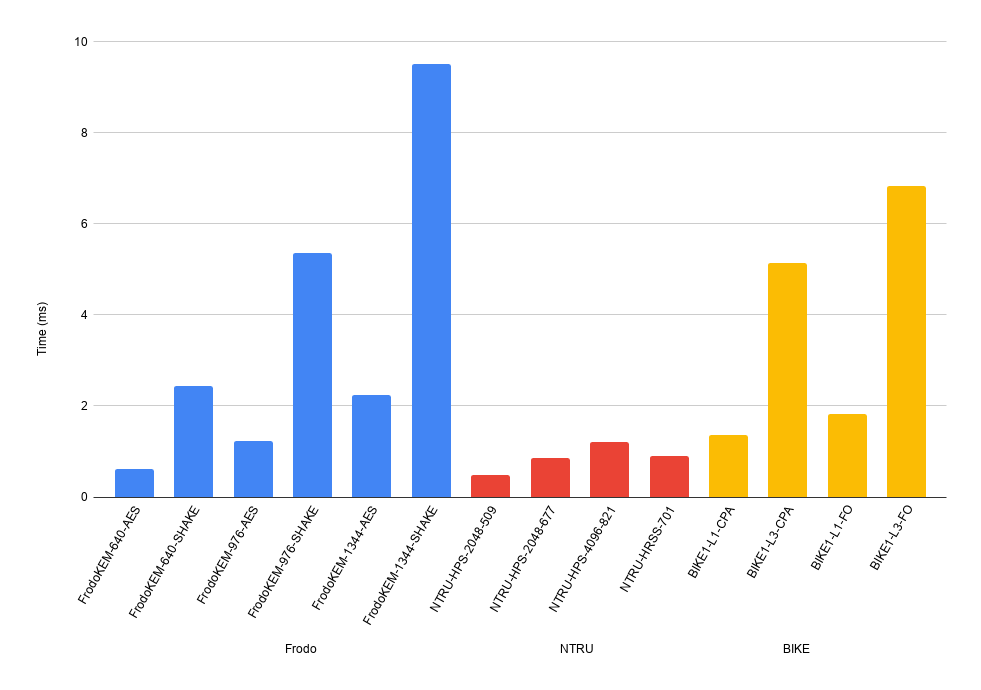
\includegraphics[scale=0.5]{tesina_SPHINCS/img/chartDecaps.png}}
% otherwise see the example in the following (commented out) line
% to scale it 50% (e.g. 20pt font get scaled to 10pt font)
%   \centerline{\includegraphics[scale=0.5]
% if you have a picture (i.e. no text hence no font size problem)
% you can fit it relatively to the page width
%   \centerline{\includegraphics[width=0.9\textwidth]
\caption{Times for performing Encaps and Decaps operations of post-quantum key exchange algorithms. On the top chart, Encaps times in $ms$ are shown, while on the bottom chart, Decaps times in $ms$ are shown.}
\label{fig:chartED}
\end{figure}

\begin{figure}
% If the picture uses fonts of the correct size (10 ... 12 pt)
% then it can be included without scaling
\centerline{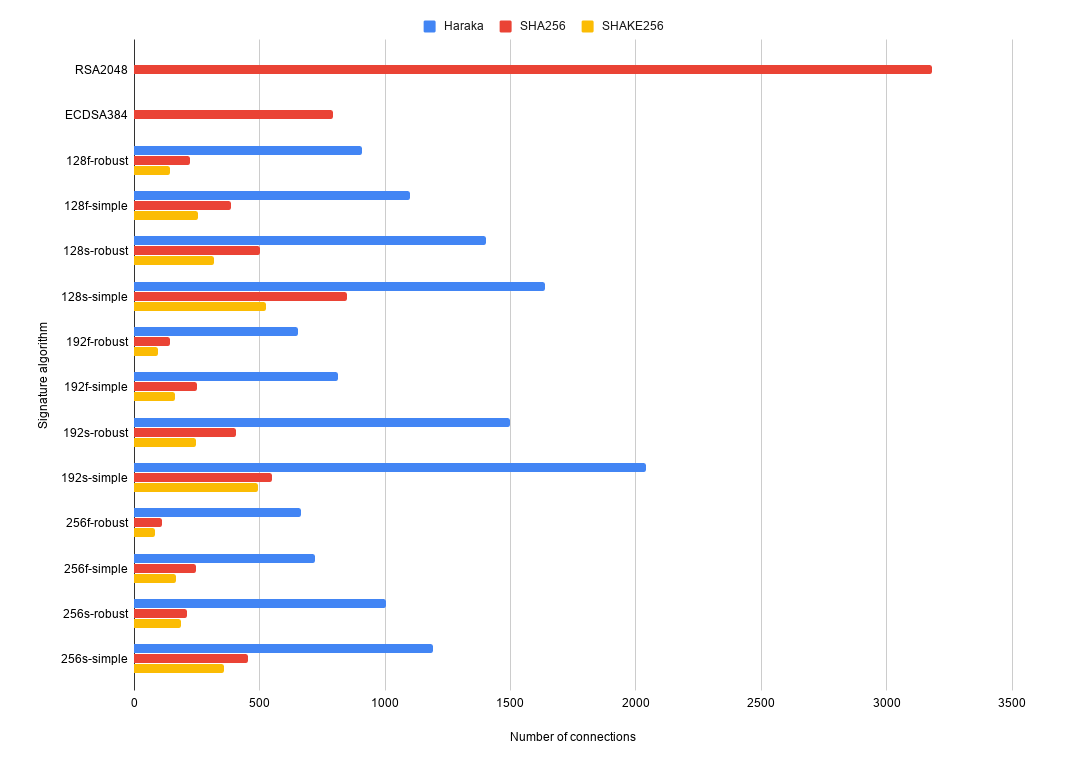
\includegraphics[scale=0.5]{tesina_SPHINCS/img/chartDH.png}}
% otherwise see the example in the following (commented out) line
% to scale it 50% (e.g. 20pt font get scaled to 10pt font)
%   \centerline{\includegraphics[scale=0.5]
% if you have a picture (i.e. no text hence no font size problem)
% you can fit it relatively to the page width
%   \centerline{\includegraphics[width=0.9\textwidth]
\caption{Number of TLS connections established in 1 second with the specified SPHINCS+ variant as authentication mechanism, grouped by parameter values. TLS handshakes are performed with the Diffie-Hellman key exchange.}
\label{fig:chartDH}
\end{figure}

\begin{figure}
% If the picture uses fonts of the correct size (10 ... 12 pt)
% then it can be included without scaling
\centerline{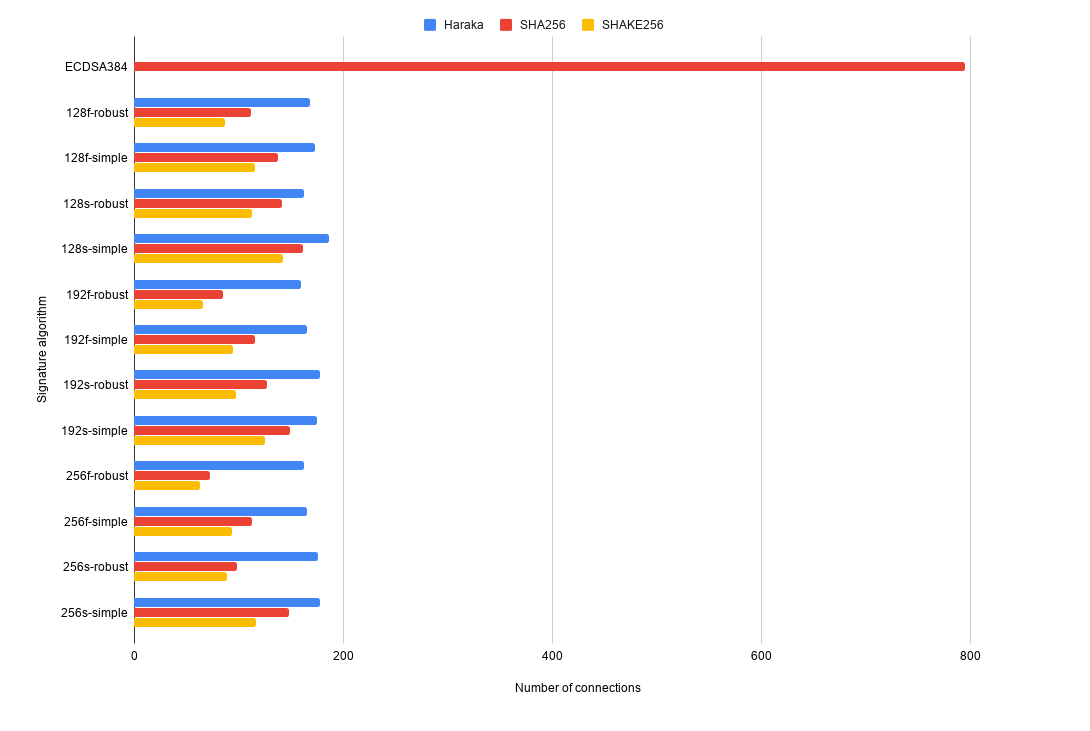
\includegraphics[scale=0.5]{tesina_SPHINCS/img/chartPQ.png}}
% otherwise see the example in the following (commented out) line
% to scale it 50% (e.g. 20pt font get scaled to 10pt font)
%   \centerline{\includegraphics[scale=0.5]
% if you have a picture (i.e. no text hence no font size problem)
% you can fit it relatively to the page width
%   \centerline{\includegraphics[width=0.9\textwidth]
\caption{Number of TLS connections established in 1 second with the specified SPHINCS+ variant, grouped by parameter values. In this chart, TLS handshakes are performed with the NTRU hps204850 post-quantum key exchange.}
\label{fig:chartPQ}
\end{figure}

%openssl results
For what concerns the ``openssl" part of the testbed, we divided the results obtained by the number of security bits provided by each variant. We concentrated variants with same parameters together. In \myfig{\ref{fig:chartDH}}, the number of connections established with each signature algorithm are shown. 
In this chart, standard signature like RSA and ECDSA are compared to post-quantum SPHINCS+ signatures. 

We can notice that RSA is at least two times faster than all of the SPHINCS+ signatures, except for the SPHINCS+-192s-simple variant. Instead, comparing these results to the number of connections established with ECDSA, these values are comparable. ECDSA384 is practically faster than all SPHINCS+ variants exploiting SHA256 and SHAKE256 hash functions. Instead its value is less than most of SPHINCS+ variants that exploit the Haraka hash function, which is on average the fastest one as shown by the results of the ``liboqs" testbed.

In the second graph instead, in \myfig{\ref{fig:chartPQ}}, the number of connections established with a post-quantum TLS handshake are shown. In this chart, the connections established with the post-quantum SPHINCS+ signatures are compared to the ECDSA384 signature scheme. Since RSA2048 is much more faster than all the other signature schemes, it was removed from this graph in order to have a clearer view.

Adding a post-quantum key exchange mechanism, instead of the Diffie-Hellman one, increases the TLS handshake time significantly, even if the chosen key exchange mechanism is the fastest one among the post-quantum algorithms tested, NTRU. A classical TLS handshake, with ECDSA, is more than 4 times faster than the most efficient post-quantum TLS handshake, which is the one performed with SPHINCS+-Haraka-128s-simple variant and NTRU hps204850 key exchange. 

Finally, recall that in all ``openssl" tests a single certificate was issued and sent from the server to the client. This represents the scenario where a self-signed certificate is used.
This experiment could be expanded using longer certificate chains with intermediate Certification Authorities, as suggested also by \cite{6_NISTPQC_TLS_SSH}. Basing on our results, the usage of long certificate chains would have a significant impact on the total handshake time, and so on the number of connection established per second.

\subsection{Discussion}
\label{sub:discussion}

In this work, we evaluated the impact of using the SPHINCS+ framework to establish TLS connections. We showed that the impact of post-quantum signatures is not negligible compared to conventional RSA or ECDSA signatures used today during a TLS handshake. We also showed that the signer will be more impacted than the verifier exploiting SPHINCS+ signed certificates.

All these considerations were made targeting the TLS communication protocol, but post-quantum signatures could be used also in other use cases. In order to provide security against quantum attacks, post-quantum signatures could be used for authenticated tunnels, as for example IPsec \cite{5_postquantum_signature_usecase}.
The implementation of post-quantum signatures is possible both for IPsec and for TLS. This is because the IPsec and the TLS protocols support fragmentation mechanisms that allow to have larger signatures. The protocol works creating larger certificate chains, and so slowing down the time needed for establishing a secure tunnel \cite{53_AuthTests}.

The introduction of post-quantum authentication, as showed before, introduces a significant overhead in terms of time. This would not be a problem for applications with low connection rates and tunnels that stay up for some time, while it would be problematic for applications that establish short and fast connections.

An example of applications with low connection rates and lasting tunnels are IPsec VPN tunnels. Since these stay on for long periods of time, increasing the time for establishing a connection to few seconds would not have such a big impact on the tunnel \cite{53_AuthTests}: once the tunnel is established, post-quantum authentication is no longer used. 

For what concerns applications that establish short and fast connections, an example can be provided with web connections. Web connections are typically short-lived. On average, the number of HTTP page requests to load a web page is about 70 requests.
If some of these requests should be performed over new TLS connections, using post-quantum authentication would have a significant impact on the HTTP performance \cite{53_AuthTests}.

\section{Conclusions}

In this work we mainly worked on SPHINCS and the reason why it is relevant to discuss about it as a post-quantum algorithm for digital signatures. First we introduced the concept of post-quantum cryptography, analysing the need of PQC, the rise of quantum computing and the projects that are currently going on in this direction, as for example the NIST post-quantum crypto project. Later we presented the main categories of post-quantum algorithms: multivariate, lattice-based, code-based and hash-based algorithms.
Among these, we selected hash-based schemes. Those schemes are used for post-quantum signatures. 
In the HBS chapter we presented the various primitives of these schemes, their statefulness property and the main advantages that a HBS has.

Later on, we focused on SPHINCS and its enhanced version SPHINCS+. About SPHINCS, we described its main components, and we presented its global construction, along with its key generation, signature and verification algorithms. For SPHINCS+, starting from SPHINCS, we pointed out the main enhancements and improvements implemented in this version, that solved some of the original SPHINCS limitations.

After that, we had a brief overview on what are the main SPHINCS+ criticalities, talking about hash function vulnerabilities, differential power analysis attacks and fault injection attacks against the SPHINCS framework.

In the last part of this work we described a use case scenario in which SPHINCS+ could be used: the TLS protocol. 
At first, we had a brief overview on both the TLS protocol and the X.509 standard for digital certificates. After that, we described how SPHINCS+ could be integrated in the context of TLS, modifying the authentication phase of the protocol in order to sign certificates with a SPHINCS+ signature. With this integration, we described the workflow of a post-quantum typical TLS connection. 
After a brief overview on the Open Quantum Safe project, a software framework for PQC, we focused on testing.
We evaluated the implementations of post-quantum authentication in TLS 1.3, exploiting a fork of the OpenSSL 1.1.1 library. 
We also provided an analysis of TLS connections established through post-quantum key exchange and signature algorithms, compared with connections established through standard key exchange mechanism coupled with post-quantum authentication.
To achieve this result, we first presented our testbed design in details. Then, results for RSA, ECDSA and SPHINCS+ signature algorithms were presented, along with post-quantum key exchange results.
Moreover, results for standard and post-quantum TLS handshakes were analysed, exploiting RSA, ECDSA and SPHINCS+ as signature mechanisms and DH and NTRU as key exchange mechanisms.
These results showed the significant overhead introduced by post-quantum authentication, in particular by the SPHINCS+ algorithm. On average, a TLS handshake with post-quantum authentication takes at least twice the time needed for a TLS handshake RSA-based. While the Haraka hash function provides fast TLS connections, comparable to ECDSA ones, the other two hash functions make SPHINCS+ authentication much slower than RSA and ECDSA authentication mechanisms. Moreover, post-quantum TLS handshakes, performed with the post-quantum NTRU key exchange, are at least 4 times slower than TLS connections established with classical cryptography.

Finally, we gave a general overview about other communication protocols in which post-quantum authentication could be implemented, as for example IPsec.

%\newpage

\begin{thebibliography}{99}
%
% Citations will be numbered according to the order
% in which they are listed in this section.
%

\bibitem{0_historyQC}
S.Bone and M.Castro,
``A Brief History of Quantum Computing'',
Quantum Computing: An Applied Approach,
pp.~11-16,
Springer, Cham,
2019,
\doi{10.1007/978-3-030-23922-0_2}

\bibitem{4_wings}
S.Kolbl,
``Putting Wings on SPHINCS'',
9th International Workshop on Post-Quantum Cryptography,
Fort Lauderdale (FL, USA),
April 9-11, 2018,
pp.~205-226,
\doi{10.1007/978-3-319-79063-3_10}

\bibitem{55_crypto}
N.Gisin, G.Ribordy, W.Tittel, and H.Zbinden,
``Quantum cryptography'',
Reviews of Modern Physics,
vol. 74,
March 2002,
pp.~145-195,
\doi{10.1103/revmodphys.74.145}

\bibitem{10_postquantum_keyexchange}
D.Stebila and M.Mosca,
``Post-Quantum Key Exchange for the Internet and the Open Quantum Safe Project'',
SAC 2016: Selected Areas in Cryptography,
St. John's (Canada),
August 10-12, 2016,
pp.~14-37,
\doi{10.1007/978-3-319-69453-5_2}

\bibitem{15_ShorPolynomial}
P.W.Shor,
``Polynomial-Time Algorithms for Prime Factorization and Discrete Logarithms on a Quantum Computer'',
SIAM Journal on Scientific Computing,
vol. 26,
October 1997,
pp.~1484-1509,
\doi{10.1137/S0097539795293172}

\bibitem{14_bernsteinPQC}
D.J.Bernstein,
``Introduction to post-quantum cryptography'',
Post-Quantum Cryptography (D.J.Bernstein, J.Buchmann, and E.Dahmen, eds.),
pp.~1-14,
Springer,
2009,
\doi{10.1007/978-3-540-88702-7_1}

\bibitem{16_Quantum}
S.Prashant,
``A Study on the basics of Quantum Computing'',
December 7, 2005,
\url{https://arxiv.org/abs/quant-ph/0511061}

\bibitem{38_BeniofTuringQuantum}
P.Benioff,
``The computer as a physical system: A microscopic quantum mechanical Hamiltonian model of computers as represented by Turing machines'',
Journal of Statistical Physics,
vol. 22,
May 1980,
pp.~563-591,
\doi{10.1007/BF01011339}

\bibitem{40_ChurchTuring}
S.Kundu, R.Kundu, S.Kundu, A.Bhattachaijee, S.Gupta, S.Ghosh, and I.Basu,
``Quantum computation: From Church-Turing thesis to Qubits'',
UEMCON 2016: IEEE 7th Annual Ubiquitous Computing, Electronics \& Mobile Communication Conference,
New York (NY, USA),
October 20-22, 2016,
pp.~1-5,
\doi{10.1109/UEMCON.2016.7777805}

\bibitem{41_ShorIbm}
L.M.K.Vandersypen, M.Steffen, G.Breyta, C.S.Yannoni, M.H.Sherwood, and I.L.Chuang,
``Experimental realization of Shor's quantum factoring algorithm using nuclear magnetic resonance'',
Nature,
vol. 414,
December 2001,
pp.~883-887,
\doi{10.1038/414883a}

\bibitem{42_Photonic}
C.Y.Lu, D.E.Browne, T.Yang, and J.W.Pan,
``Demonstration of a Compiled Version of Shor's Quantum Factoring Algorithm Using Photonic Qubits'',
Physical Review Letters,
vol. 99,
December 2007,
\doi{10.1103/PhysRevLett.99.250504}

\bibitem{43_EntanglementQC}
B.P.Lanyon, T.J.Weinhold, N.K.Langford, M.Barbieri, D.F.V.James, A.Gilchrist, and A.G.White,
``Experimental Demonstration of a Compiled Version of Shor's Algorithm with Quantum Entanglement'',
Physical Review Letters,
vol. 99,
January 2008,
\doi{10.1103/PhysRevLett.99.250505}

\bibitem{44_Factorization21}
E.M.Lopez, A.Laing, T.Lawson, R.Alvarez, X.Q.Zhou and J.L.O'Brien,
``Experimental realization of Shor's quantum factoring algorithm using qubit recycling'',
Nature Photon,
vol. 6,
October, 2012,
pp.~773-776,
\doi{10.1038/nphoton.2012.259}

\bibitem{54_rsa2048}
C.Gidney and M.Ekera,
``How to factor 2048 bit RSA integers in 8 hours using 20 million noisy qubits'',
May 23, 2019,
\url{https://arxiv.org/abs/1905.09749}

\bibitem{5_postquantum_signature_usecase}
P.Kampanakis and D.Sikeridis,
``Two Post-Quantum Signature Use-cases:
Non-issues, Challenges and Potential Solutions'',
7th ETSI/IQC Quantum Safe Cryptography Workshop, 
Seattle (WA, USA),
November 5-7, 2019,
\url{https://eprint.iacr.org/2019/1276.pdf}

\bibitem{9_postquantum_auth_openssl}
D.Butin, J.Walde, and J.Buchmann,
``Post-Quantum Authentication in OpenSSL with
Hash-Based Signatures'',
ICMU 2017: IEEE Tenth International Conference on Mobile Computing and Ubiquitous Network,
Toyama (Japan),
October 3-5, 2017,
pp.~1-6,
\doi{10.23919/ICMU.2017.8330093}

\bibitem{18_NISTreport}
G.Alagic, J.M.Alperin-Sheriff, D.C.Apon, D.A.Cooper, Q.H.Dang, C.A.Miller, D.Moody, R.C.Peralta, R.A.Perlner, A.Y.Robinson, D.C.Smith-Tone, and Y.K.Liu,
``Status Report on the First Round of the NIST Post-Quantum Cryptography Standardization Process'',
NIST Interagency/Internal Report,
vol. 8240,
January 31, 2019,
\doi{10.6028/NIST.IR.8240}

\bibitem{6_NISTPQC_TLS_SSH}
E.Crockett, C.Paquin, and D.Stebila,
``Prototyping post-quantum and hybrid key exchange and authentication in TLS and SSH'',
NIST 2nd PQC Standardization Conference,
Santa Barbara (CA, USA),
August 22-25, 2019,
\url{https://eprint.iacr.org/2019/858}

\bibitem{1_sphincspaper}
D.J.Bernstein, D.Hopwood, A.Huelsing, T.Lange, R.Niederhagen, L.Papachristodoulou, M.Schneider, P.Schwabe, and Z.Wilcox-O'Hearn,
``SPHINCS: practical stateless hash-based signatures'',
EUROCRYPT 2015: Advances in Cryptology,
Sofia (Bulgaria),
April 26-30, 2015,
pp.~368-397,
\doi{10.1007/978-3-662-46800-5_15}

\bibitem{21_multivariate}
J.Ding and B.Y.Yang,
``Multivariate Public Key Cryptography'',
Post-Quantum Cryptography (D.J.Bernstein, J.Buchmann, and E.Dahmen, eds.),
pp.~193-241,
Springer,
2009,
\doi{10.1007/978-3-540-88702-7_6}

\bibitem{22_HFE}
J.Patarin,
``Hidden Field Equations (HFE) and Isomorphisms of Polynomials (IP): two new Families of Asymmetric Algorithms'',
EUROCRYPT 1996: Advances in Cryptology,
Saragossa (Spain),
May 12-16, 1996,
pp.~33-48,
\doi{10.1007/3-540-68339-9_4}

\bibitem{23_unbalancedvinegar}
A.Kipnis, J.Patarin, and L.Goubin,
``Unbalanced Oil and Vinegar Signature Schemes'',
EUROCRYPT 1999: Advances in Cryptology, 
Prague (Czech Republic),
May 2-6, 1999,
pp.~206-222,
\doi{10.1007/3-540-48910-X_15}

\bibitem{24_LWE}
R.Lindner and C.Peikert,
``Better Key Sizes (and Attacks) for LWE-Based Encryption'',
CT-RSA 2011: Topics in Cryptology,
San Francisco (CA, USA),
February 14-18, 2011,
pp.~319-339,
\doi{10.1007/978-3-642-19074-2_21}

\bibitem{26_code_based}
N.Sendrier,
``Code-Based Cryptography'',
Post-Quantum Cryptography (D.J.Bernstein, J.Buchmann, and E.Dahmen, eds.),
pp.~95-145,
Springer,
2009,
\doi{10.1007/978-1-4419-5906-5}

\bibitem{27_Eliece}
R.J.McEliece,
``A Public-Key Cryptosystem Based on Algebraic Coding Theory'',
DSN Progress Report 42-44,
February 1978,
pp.~114-116,
\url{https://tmo.jpl.nasa.gov/progress_report2/42-44/44N.PDF}

\bibitem{29_ElieceCryptosystem}
N.Sendrier,
``McEliece Public Key Cryptosystem'',
Encyclopedia of Cryptography and Security (H.C.A.van Tilborg, S.Jajodia, eds),
pp.~767-768,
Springer,
2011,
\doi{10.1007/978-1-4419-5906-5}

\bibitem{28_CodeAttacks}
H.Dinh, C.Moore, and A.Russell,
``McEliece and Niederreiter Cryptosystems That Resist Quantum Fourier Sampling Attacks'',
CRYPTO 2011: Advances in Cryptology,
Santa Barbara (CA, USA),
August 14-18, 2011,
pp.~761-779,
\doi{10.1007/978-3-642-22792-9_43}

\bibitem{30_Merkle}
R.C.Merkle,
``A Certified Digital Signature'',
CRYPTO 1989: Advances in Cryptology,
Santa Barbara (CA, USA),
August 20-24, 1989,
pp.~218-238,
\doi{10.1007/0-387-34805-0_21}

\bibitem{31_Lamport}
L.Lamport,
``Constructing Digital Signatures from a One Way Function'',
SRI International Computer Science Laboratory,
October 18, 1979,
\url{https://www.microsoft.com/en-us/research/uploads/prod/2016/12/Constructing-Digital-Signatures-from-a-One-Way-Function.pdf}

\bibitem{3_SPHINCS_secondpaper}
D.J.Bernstein, A.Huelsing, S.Kolbl, R.Niederhagen, J.Rijneveld,  and P.Schwabe,
``The SPHINCS+ Signature Framework'',
CCS 2019: ACM SIGSAC Conference on Computer and Communications Security,
London (UK),
November 11-15, 2019,
pp.~2129-2146,
\doi{10.1145/3319535.3363229}

\bibitem{12_faultinjection}
A.Genet, M.J.Kannwischer, H.Pelletier, and A.McLauchlan,
``Practical Fault Injection Attacks on SPHINCS'',
IACR Cryptology ePrint Archive,
2018,
\url{https://eprint.iacr.org/2018/674}

\bibitem{7_hashbased}
G.Endignoux,
``Design and implementation of a post-quantum hash-based cryptographic signature scheme'',
Master's Thesis,
July 2017,
\url{https://gendignoux.com/assets/pdf/2017-07-master-thesis-endignoux-report.pdf}

\bibitem{2_SPHINCS+_round2}
J.P.Aumasson, D.J.Bernstein, C.Dobraunig,
M.Eichlseder, S.Fluhrer, S.L.Gazdag, A.Huelsing,
P.Kampanakis, S.Kolbl, T.Lange, M.M.Lauridsen,
F.Mendel, R.Niederhagen, C.Rechberger, J.Rijneveld,
and P.Schwabe,
``SPHINCS+ Submission to the NIST post-quantum project'',
2017,
\url{https://sphincs.org/data/sphincs+-specification.pdf}

\bibitem{32_XMSS}
J.Buchmann, E.Dahmen, and A.Huelsing,
``XMSS - A Practical Forward Secure Signature Scheme based on Minimal Security Assumptions'',
PQCrypto 2011: Post-Quantum Cryptography,
Taipei (Taiwan),
November 29-December 2, 2011,
pp.~117-129,
\doi{10.1007/978-3-642-25405-5_8}

\bibitem{33_RFC_XMSS}
A.Huelsing, D.Butin, S.Gazdag, J.Rijneveld, and A.Mohaisen,
``XMSS: eXtended Merkle Signature Scheme'',
\rfc{8391},
May 2018,
\doi{10.17487/RFC8391}

\bibitem{34_birthday}
J.Katz and Y.Lindell,
``Introduction to Modern Cryptography, 2nd Edition'',
Chapman and Hall CRC,
2014

\bibitem{13_faultattacks}
L.Castelnovi, A.Martinelli, and T.Prestm,
``Grafting Trees: a Fault Attack against the SPHINCS framework'',
PQCrypto 2018: Post-Quantum Cryptography,
Fort Lauderdale (FL, USA),
April 9-11, 2018,
pp.~165-184,
\doi{10.1007/978-3-319-79063-3_8}

\bibitem{53_hbs}
D.Wong,
Hash-Based Signatures,
\url{https://cryptoservices.github.io/quantum/2015/12/04/one-time-signatures.html},
December 4, 2015

\bibitem{35_Song}
F.Song,
``A Note on Quantum Security for Post-Quantum Cryptography'',
PQCrypto 2014: Post-Quantum Cryptography,
Waterloo (Canada),
October 1-3, 2014,
pp.~246-265,
\doi{10.1007/978-3-319-11659-4_15}

\bibitem{45_ShortOTS}
G.M.Zaverucha and D.R.Stinson,
``Short One-Time Signatures'',
IACR Cryptology ePrint Archive,
2010,
\url{https://eprint.iacr.org/2010/446}

\bibitem{46_WOTSvariant}
J.Buchmann, E.Dahmen, S.Ereth, A.Huelsing, and M.Ruckert,
``On the Security of the Winternitz One-Time Signature Scheme'',
AFRICACRYPT 2011: Progress in Cryptology,
Dakar (Senegal),
July 5-7, 2011,
pp.~363-378,
\doi{10.1007/978-3-642-21969-6_23}

\bibitem{48_WOTS+}
A.Huelsing,
``WOTS+ - Shorter Signatures for Hash-Based Signature Schemes'',
AFRICACRYPT 2013: Progress in Cryptology,
Cairo (Egypt),
June 22-24, 2013,
pp.~173-188,
\doi{10.1007/978-3-642-38553-7}

\bibitem{47_MultipleTimes}
J.Pieprzyk, H.Wang, and C.Xing,
``Multiple-Time Signature Schemes against Adaptive Chosen Message Attacks'',
SAC 2003: Selected Areas in Cryptography,
Ottawa (Canada),
August 14-15, 2003,
pp.~88-100,
\doi{10.1007/978-3-540-24654-1_7}

\bibitem{49_HORS}
L.Reyzin and N.Reyzin,
``Better than BiBa: Short One-time Signatures with Fast Signing and Verifying'',
ACISP 2002: Information Security and Privacy,
Melbourne (Australia),
July 3-5, 2002,
pp.~144-153,
\doi{10.1007/3-540-45450-0_11}

\bibitem{37_RFC_LMS}
D.McGrew, M.Curcio, and S.Fluhrer,
``Leighton-Micali Hash-Based Signatures'',
\rfc{8554},
April 2019,
\doi{10.17487/RFC8554}

\bibitem{36_Grover}
C.Zalka,
``Grover's quantum searching algorithm is optimal'',
Physical Review A,
vol. 60,
October 1999,
pp.~2746-2751,
\doi{10.1103/PhysRevA.60.2746}

\bibitem{8_ARM}
A.Huelsing, J.Rijneveld, and P.Schwabe,
``ARMed SPHINCS Computing a 41 KB signature in 16 KB of RAM'',
IACR Cryptology ePrint Archive,
2015,
\url{https://eprint.iacr.org/2015/1042.pdf}

\bibitem{50_Goldreich}
O.Goldreich,
``Foundations of Cryptography: Volume 2 Basic Applications'',
Cambridge University Press,
2009

\bibitem{11_poweranalysis}
M.J.Kannwischer, A.Genet, D.Butin, J.Kramer, and J.Buchmann,
``Differential Power Analysis of XMSS and SPHINCS'',
COSADE 2018: Constructive Side-Channel Analysis and Secure Design,
Singapore,
April 23-24, 2018,
pp.~168-188,
\doi{10.1007/978-3-319-89641-0_10}

\bibitem{51_MultiTarget}
A.Huelsing, J.Rijneveld, and F.Song,
``Mitigating Multi-Target Attacks in Hash-based Signatures'',
PKC 2016: Public-Key Cryptography PKC,
Taipei (Taiwan),
March 6-9, 2016,
pp.~387-416,
\doi{10.1007/978-3-662-49384-7_15}

\bibitem{52_SecuritySign}
L.G.Bruinderink and A.Huelsing,
``Oops, I did it again - Security of One-Time Signatures under Two-Message Attacks'',
SAC 2017: Selected Areas in Cryptography,
Ottawa (Canada),
August 16-18, 2017,
pp.~299-322,
\doi{10.1007/978-3-319-72565-9_15}

\bibitem{53_AuthTests}
D.Sikeridis, P.Kampanakis, and M.Devetsikiotis,
``Post-Quantum Authentication in TLS 1.3: A Performance Study'',
IACR Cryptology ePrint Archive,
2020,
\url{https://eprint.iacr.org/2020/071.pdf}

\end{thebibliography}

\appendix

\section{User's Manual}
\label{sec:usermanual}

This appendix provides some instructions on how to use the testbed developed during this work. 
The repository for this work\footnote{\url{https://git-sec.polito.it/post-quantum-crypto/sphincs-tls}} contains all scripts useful to produce the statistics analysed inside Section \ref{sec:test}.
In the repository, a detailed description of the testbed can be found inside the README document.
All of these scripts are also attached to this work.

To replicate our test case scenario, the following steps need to be taken: 
\begin{enumerate}
    \item Make sure you have Ubuntu 18.04 LTS installed. Our tests were made on Ubuntu 18.04.5 LTS. The testbed is not ensured to work with previous versions of Ubuntu;
    \item Clone the repository inside a directory or download the \textit{tests} directory from the git repository mentioned above;
    \item Move the \textit{tests} directory inside your home. This is mandatory at the time of the writing of this user manual, since the testbed is currently working with absolute paths;
    \item After giving execution permissions to all .sh scripts, they can be executed just typing \textit{./script.sh} from the \textit{tests} folder.
\end{enumerate}

The testbed contained into the \textit{tests} folder is divided in two sections: 
\begin{itemize}
    \item \textbf{liboqs}. With this part both liboqs and OpenSSL libraries are installed.
    With these scripts, SPHINCS+ along with all its variants is tested and compared to standard signature schemes: RSA and ECDSA.
    This is done exploiting the liboqs test suite library. Also the OpenSSL one is installed because standard cryptographic algorithms can not be tested directly through the liboqs test suite.
    The results comprehend data about the times of key generation, sign and verify operations for signature algorithms and of encapsulation and decapsulation operations for key exchange algorihtms.
    This part includes the following scripts: \textit{build\_testbed\_liboqs.sh}, \textit{run\_testbed\_liboqs.sh}, \textit{run\_testbed\_liboqs\_rsaecdsa.sh} and  \textit{clean\_testbed\_liboqs.sh}.
    \item \textbf{OpenSSL}. This is the fundamental part of the testbed. Mainly, it computes the number of TLS connections established between a client and a server. These connections are performed in three ways: with standard signature algorithms (RSA and ECDSA) and standard key exchange algorithms (Diffie-Hellman), with post-quantum signature algorithms (SPHINCS+ and all its variants) and standard key exchange algorithms (Diffie-Hellman), with post-quantum signature algorithms (SPHINCS+ and all its variants) and post-quantum key exchange algorithms (NTRU).
    This part includes the following scripts: \textit{build\_testbed.sh}, \textit{build\_testbed\_single\_variant.sh}, \textit{run\_testbed.sh}, \textit{run\_testbed\_rsaecdsa.sh} and \textit{clean\_testbed.sh}.
\end{itemize}

For what concerns the results produced by those scripts, they are organised in files inside \textit{tests/results} folder.
All files related to the first part of the testbed, the one described in the \textbf{liboqs} section, are in the format \textit{output\_liboqs\_*.txt}. All files related to the second part of the testbed, \textbf{OpenSSL}, the one focusing on TLS integration, are in the format \textit{output\_tls\_s\_time\_*.txt}.

\section{Programmer's Manual}
\label{sec:programmermanual}

In this last section of the appendix, we provide additional information about the code of our testbed and its working.

As explained also in \ref{sec:usermanual}, the testbed\footnote{The code of our testbed has been linked in the User's Manual, see Section \ref{sec:usermanual}.} is composed by 9 scripts written in bash. They are all .sh files and they are contained into a \textit{tests} directory. 
In order to use this testbed, it must be downloaded and installed it into home directory ($\sim$). This step is required because some scripts use absolute paths to work. In order to change this behaviour it is possible to change the paths inside the scripts, if necessary. By default, the path for one of the scripts should be \textit{$\sim$/tests/script\_name.sh}.

All scripts need read and execute permission to execute and they can be run directly by command line with no parameters. Some of these scripts allow for one parameter, in order to customise the target algorithm of the execution. Information about which script accept this customisation can be found in the documentation of the code.
As mentioned before, the testbed is divided into a \textbf{liboqs} part and a \textbf{openssl} part. 
Scripts referring to the first part are identified by the ``testbed\_liboqs" keywords. Scripts referring to the second part are identified just by the ``testbed" keyword.
Moreover, individual scripts can be divided into ``build", ``run" and ``clean" scripts.

For the \textbf{liboqs} part, we present a summary of the main features of each script:
\begin{itemize}
    \item \textit{build\_testbed\_liboqs.sh}: downloads both liboqs and OpenSSL libraries inside an ad-hoc directory, called \textit{testbed\_for\_liboqs\_tests}, and compiles them. The liboqs is compiled to have as default signature algorithm SPHINCS+-Haraka-128f-robust. This is used to issue X.509 certificates. In this way if the library needs to be used afterward, it is ready to be tested.
    \item \textit{run\_testbed\_liboqs.sh}: runs the test suites provided by the liboqs library for post-quantum algorithms. All SPHINCS+ variants are tested with the \textit{test\_sig} script inside liboqs. Moreover, post-quantum KEMs like BIKE, Frodo and NTRU are tested with the \textit{test\_kem} script inside liboqs.
    \item \textit{run\_testbed\_liboqs\_rsaecdsa.sh}: runs multiple times (10) the openssl speed command for evaluating the performance of RSA2048 and ECDSA384 algorithms.
    \item \textit{clean\_testbed\_liboqs.sh}: deletes the \textit{testbed\_for\_liboqs\_tests} directory.
\end{itemize}

Moreover, here we present a summary of the features of the scripts belonging to the \textbf{openssl} part of the testbed:
\begin{itemize}
    \item \textbf{\textit{build\_testbed.sh}}: iterates on the list of all SPHINCS+ variants (36). For each of them, it compiles the liboqs with the current variant as the default signature algorithm. Then both the liboqs and openssl libraries are built. It then calls the \textit{run\_testbed.sh} script passing as parameter the current SPHINCS+ variant. Then, if the available space of the current machine is not enough to support multiple copies of the liboqs and openssl libraries, it calls the \textit{clean\_testbed.sh} script. Those libraries have to be rebuilt for each SPHINCS+ variant since the implementation of SPHINCS+ into OpenSSL is not available yet. The only way to test it into the TLS scenario is to compile the liboqs library with SPHINCS+ as the default signature algorithm.
    \item \textit{build\_testbed\_single\_variant.sh}: enables to build the liboqs and openssl libraries selecting as the default signature algorithm the one specified in the command line as first parameter. The algorithm has to be specified in the form \textit{OQS\_SIG\_alg\_sphincs\_haraka\_128f\_robust}.
    \item \textit{run\_testbed.sh}: tests a single SPHINCS+ variant, passed as first parameter by command line. It launches a TLS server and evaluates the performance of the TLS handshake with the \textit{s\_time} command, multiple times (10). For each SPHINCS+ variant, the TLS handshake is performed with the Diffie-Hellman key exchange and with the NTRU hps2048509 post-quantum key exchange algorithm.
    \item \textit{run\_testbed\_rsaecdsa.sh}: evaluates the performances of TLS handshakes performed with RSA2048 and ECDSA384 signature algorithms. For each signature algorithm, it creates inside openssl the keys and the X.509 certificates, and then iterates multiple times (10) executing the \textit{s\_time} command.
    \item \textit{clean\_testbed.sh}: deletes the \textit{testbed} directory.
\end{itemize}

Finally, as mentioned in \ref{sec:usermanual}, recall that all outputs produced by those scripts, if any, can be found inside the \textit{tests/results} directory.

\end{document}
%
% Before delivering your report, don't forget to run a spell checker,
% such as aspell (with a UK-english dictionary)
%
